%% Copernicus Publications Manuscript Preparation Template for LaTeX Submissions
%% ---------------------------------
%% This template should be used for copernicus.cls
%% The class file and some style files are bundled in the Copernicus Latex Package, which can be downloaded from the different journal webpages.
%% For further assistance please contact Copernicus Publications at: production@copernicus.org
%% https://publications.copernicus.org/for_authors/manuscript_preparation.html


%% Please use the following documentclass and journal abbreviations for preprints and final revised papers.

%% 2-column papers and preprints
\documentclass[bg, manuscript]{copernicus}



%% Journal abbreviations (please use the same for preprints and final revised papers)


% Advances in Geosciences (adgeo)
% Advances in Radio Science (ars)
% Advances in Science and Research (asr)
% Advances in Statistical Climatology, Meteorology and Oceanography (ascmo)
% Annales Geophysicae (angeo)
% Archives Animal Breeding (aab)
% ASTRA Proceedings (ap)
% Atmospheric Chemistry and Physics (acp)
% Atmospheric Measurement Techniques (amt)
% Biogeosciences (bg)
% Climate of the Past (cp)
% DEUQUA Special Publications (deuquasp)
% Drinking Water Engineering and Science (dwes)
% Earth Surface Dynamics (esurf)
% Earth System Dynamics (esd)
% Earth System Science Data (essd)
% E&G Quaternary Science Journal (egqsj)
% European Journal of Mineralogy (ejm)
% Fossil Record (fr)
% Geochronology (gchron)
% Geographica Helvetica (gh)
% Geoscience Communication (gc)
% Geoscientific Instrumentation, Methods and Data Systems (gi)
% Geoscientific Model Development (gmd)
% History of Geo- and Space Sciences (hgss)
% Hydrology and Earth System Sciences (hess)
% Journal of Bone and Joint Infection (jbji)
% Journal of Micropalaeontology (jm)
% Journal of Sensors and Sensor Systems (jsss)
% Magnetic Resonance (mr)
% Mechanical Sciences (ms)
% Natural Hazards and Earth System Sciences (nhess)
% Nonlinear Processes in Geophysics (npg)
% Ocean Science (os)
% Polarforschung - Journal of the German Society for Polar Research (polf)
% Primate Biology (pb)
% Proceedings of the International Association of Hydrological Sciences (piahs)
% Scientific Drilling (sd)
% SOIL (soil)
% Solid Earth (se)
% The Cryosphere (tc)
% Weather and Climate Dynamics (wcd)
% Web Ecology (we)
% Wind Energy Science (wes)


%% \usepackage commands included in the copernicus.cls:
%\usepackage[german, english]{babel}
%\usepackage{tabularx}
%\usepackage{cancel}
%\usepackage{multirow}
%\usepackage{supertabular}
%\usepackage{algorithmic}
%\usepackage{algorithm}
%\usepackage{amsthm}
%\usepackage{float}
%\usepackage{subfig}
%\usepackage{rotating}

%\graphicspath{{pictures/}}
\graphicspath{{figures/}}

\begin{document}

%\title{The 2018 heatwave and its implications on ozone induced damage on vegetation in a subarctic climate}
\title{Characterizing subarctic biomes for land surface modeling of pollution and climate risk}


% \Author[affil]{given_name}{surname}

\Author[1]{Stefanie}{Falk}
\Author[2]{Ane Victoria}{Vollsnes}
\Author[2]{Aud}{Eriksen}
\Author[3]{Lisa}{Emberson}
\Author[3]{Connie}{O'Neill}
\Author[1]{Frode}{Stordal}
\Author[1]{Terje}{Koren Berntsen}

\affil[1]{Department of Geosciences, University of Oslo, Oslo, Norway}
\affil[2]{Department of Biosciences, University of Oslo, Oslo, Norway}
\affil[3]{Department of Environment and Geography, University of York, UK}

%% The [] brackets identify the author with the corresponding affiliation. 1, 2, 3, etc. should be inserted.

%% If an author is deceased, please mark the respective author name(s) with a dagger, e.g. "\Author[2,$\dag$]{Anton}{Smith}", and add a further "\affil[$\dag$]{deceased, 1 July 2019}".

%% If authors contributed equally, please mark the respective author names with an asterisk, e.g. "\Author[2,*]{Anton}{Smith}" and "\Author[3,*]{Bradley}{Miller}" and add a further affiliation: "\affil[*]{These authors contributed equally to this work.}".


\correspondence{Stefanie Falk (stefanie.falk@geo.uio.no)}

\runningtitle{Subarctic biomes for land surface modeling}

\runningauthor{Falk et al.}





\received{}
\pubdiscuss{} %% only important for two-stage journals
\revised{}
\accepted{}
\published{}

%% These dates will be inserted by Copernicus Publications during the typesetting process.


\firstpage{1}

\maketitle


\begin{abstract}
  The unique vegetation biomes of the subarctic region acclimatized to extremes of cold and midnight sun are likely to be at threat from the combined impacts of climate change and increasing ozone (\chem{O_3}) concentrations. The atmospheric and climatic characteristics of the subarctic are known to lead to pronounced peak \chem{O_3} concentrations in spring. To date, only a few studies have been conducted to assess the response of subarctic vegetation to variations in climate and air pollution, at least by comparison with other parts of Europe. This study looks to fill this knowledge gap by examining trends in climate variables and \chem{O_3} concentrations that have occurred over the past few decades. These climatological and \chem{O_3} data are used to assess the extent to which two recent years (2018 and 2019) deviate from climatic and \chem{O_3} concentration norms and how these current (and potentially more frequent future) deviations may influence \chem{O_3} damage to subarctic vegetation. We find that 2018 was an anomalous warm and bright year (in particular in spring and early summer) with higher than average \chem{O_3} concentrations in April/May and a high number of episodic peak \chem{O_3} concentration above $40\,\unit{ppb}$ in June--August, the latter in part attributable to an increase in forest fires in the Northern Hemisphere as well as warmer and sunnier conditions. We apply a flux-metric to determine \chem{O_3} risk and damage to vegetation as a function of \chem{O_3} concentration, climate variables, and species-specific physiology. We find that bespoke parameterizations of plant functional types (PFTs) for subarctic vegetation bio-types increase estimates of ozone-induced reduction of total biomass by $2.5$ to $17.4\,\unit{\%}$ in this flux-metric. Our study, suggests that assessments that use generic parameterizations are likely to underestimate the risk of \chem{O_3} damage in this region. We conclude that appropriate parameterization for the growing season and plant physiological responses to light and temperature are particularly important for accurate modeling of seasonal gas exchange. Efforts should be targeted towards accurately defining subarctic bio-type physiological response to climatic variables to improve regional and global scale biogeochemical cycling under current and future climates.
\end{abstract}

%\copyrightstatement{TEXT}  %% This section is optional and can be used for copyright transfers.

\introduction  %% \introduction[modified heading if necessary]
\label{sec:intro}

Ground-level ozone (\chem{O_3}) is a highly toxic pollutant known to cause damage to human health \citep{WHO2008} and to a variety of ecosystems around the World \citep{PT:Emberson2020}. Ozone is a cause of visible injury, photosynthetic damage, early senescence as well as programmed cell death of plants \citep{PCE:Kangasjarvi2005}. Annual global yield losses of four major crops (wheat, rice, maize, and soybean) of $3-15\,\unit{\%}$ \citep{PJ:Ainsworth2017} and a suggested loss in primary production in forestry of $7\,\unit{\%}$ \citep{GCB:Wittig2009,EP:Matyssek2012} has been attributed to ozone.
The crop yield loss studies indicate a threat to food security in rapidly developing countries, e.g., in East and South-East Asia \citep{GCB:Tang2013,NCC:Tai2014,AE:Chuwah2015,GCB:Mills2018}, where ozone concentrations related to enhanced pollutant emissions from the transport, residential, power generation, and industrial sectors have increased in the past few decades. Even though long-term (pre-1950) observations of ground-level ozone concentrations are scarce; evidence from trend analysis of those few sites suggests that since the industrial revolution, background concentrations in the northern hemisphere have at least doubled and continued to increase \citep[Chapter 2]{IPCC2013}. Recent trend analyses for Europe indicate that a maximum was reached in 2007 \citep{AE:Derwent2018}, after which tropospheric ozone started to level off or even decline \citep{ESA:Cooper2014, ACP:Wespes2018,ESA:Gaudel2018}. This can be attributed to a successful implementation of air quality regulations coupled with economic restructuring, reducing the number of episodes of peak concentrations especially in summertime over Europe and North America \citep[e.g.,][]{ESA:Fleming2018, ESA:Mills2018}. However, changes in environmental conditions associated with climate change, such as an increase in the frequency of heatwaves, could negate the effectiveness of emission reductions in relation to ozone impacts and air quality \citep{NCC:Lin2020}.

Complex photochemical cycles involving precursor gases such as carbon monoxide (\chem{CO}) and hydrocarbons known as volatile organic compounds (VOCs) in the presence of nitrogen oxides (\chem{NO_x}) lead to the formation of \chem{O_3} at ground-level. Despite a relatively short average tropospheric lifetime of approximately $22\,\unit{days}$, ranging from a few days in the tropical boundary layer to up to $1\,\unit{year}$ in the upper troposphere \citep{JGR:Stevenson2005,ACP:Young2013}, ozone and is precursors are subject to advection over long distances. Episodes of high ozone concentrations in the absence of local pollution sources can therefore often be attributed to the long-range transport of both ozone and its precursors. In northern Fennoscandia, episodes of enhanced ozone concentrations in 2003 and 2006 have been traced back to ozone precursor emissions related to forest fires in southern and eastern Europe, respectively \citep{AE:Lindskog2007,EP:Karlsson2013}. Besides VOCs from anthropogenic sources, hydrocarbons are also emitted by vegetation itself in the form of terpenes and monoterpenes, so-called biogenic volatile substances (BVOCs). These emissions are thought to be a response to factors, such as thermal stress, defense against herbivores, or even attraction of pollinators \citep{TPS:Penuelas2003}. 

In the annual cycle in Boreal climates, a distinct maximum of ground-level ozone concentrations typically occurs in spring followed by lower concentrations throughout the summer. Several conditions unique to the Arctic are stimulating the formation of this spring peak. Major pathways of ozone and its precursors' removal from the boundary layer include dry deposition on vegetated surfaces and photochemistry \citep{RG:Clifton2020}. As dry deposition to bare ground or snow and ice-covered surfaces was found to be low \citep{ACP:Helmig2007}, both pathways of removal are substantially suppressed during polar night \citep{AE:Monks2000}. This leads to a build-up of ozone and its precursors during winter. Come spring precursors are photochemically activated again, while snow cover typically continues to prevail and suppress ozone dry deposition.
On the other hand, very high ozone concentrations occurring over shorter periods can often be attributed to deep tropopause folding events over the Arctic during winter. These events facilitate an intrusion of stratospheric air masses which are enriched in ozone \citep{JGR:Skerlak2015}.
The spring peak is more pronounced in northern Fennoscandia than in more southern locations but shows a  high interannual variability \citep{AB:Klingberg2009, BER:Klingberg2019}. A cause for this is the complex interplay between atmospheric dynamics and chemistry \citep{AE:Laurila1996,BER:Hatakka2003} as described above as well as anthropogenic and biogenic activity \citep{AE:Rummukainen1996,AE:Simpson2002,QJRMS:Galbally2007,NGS:Schnell2009}. \citet{ACP:Andersson2017} showed in a modeling study focused on Fennoscandia that the variability of ozone concentrations in winter can be attributed mainly to changes in atmospheric background (transport) of ozone, while summertime abundance is mostly affected by emissions of precursors in the rest of Europe. Meteorology plays an important role throughout the year.

The start of the growing season (GS) in northern Fennoscandia has been shifting to earlier dates in response to the general warming trend \citep[e.g.]{GCB:Menzel2006,RS:Hogda2013,IJB:Karlsen2007} and thereby converging with the period of the ozone spring peak. At the same time, the growing season is also becoming longer. A longer growing season is prolonging the time in which vegetation can accumulate ozone. For natural and semi-natural vegetation which is already subject to rapid climatic changes known as Arctic amplification \citep{AMAP2012,IPCC2013}, these factors could promote a higher potential risk for northern vegetation to ozone-induced damage in the not so distant future.

Ozone acts as oxidative stress to plants. Its main action is imposed through reactions occurring in the cell walls and cell membranes of mesophyll cells inside the leaves. Ozone enters the leaves through stomata, leaf pores that enable gas exchange, allowing the entry of \chem{CO_2} for photosynthesis and loss of \chem{H_2O} vapor via the plant transpiration stream. Stomatal aperture, and hence stomatal conductance to these gases (including ozone) will vary over the day and growing season primarily to balance \chem{CO_2} uptake against \chem{H_2O} vapor loss. The higher the stomatal conductance, the higher the potential for ozone uptake. Stomatal conductance has been empirically linked to environmental factors such as air temperature $T$, photosynthetic photon flux density (PPFD), vapor pressure deficit (VPD), and soil water potential (SWP) as well as photosynthesis itself \cite[e.g.]{PTRS:Jarvis1976, BallBerry1987, Emberson2000, ICP:MappingManual2017}. Results from open-top chamber (OTC) experiments on downy birch (\emph{Betula pubescens}) and mountain birch (\emph{Betula pubescens toruosa}), native to subarctic regions, indicated reductions in both biomass, in root:shoot ratio, and visible leaf damage under elevated ozone treatment ($\left<\chem{[O_3]}\right> = 36-54\,\unit{ppb}$) \citep{Amb:Manninen2009}. Although Scots pine (\emph{Pinus sylvestris}) is considered to be more ozone tolerant due to an absence of visible injuries \citep{Amb:Girgzdiene2009}, \citet{Amb:Manninen2009} found chlorophyll:carotenoid ratio and polyamines reductions under elevated ozone concentrations indicating susceptibility to ozone also in these species.\\

A substantial body of evidence exists that suggests flux-based metrics, that relate stomatal ozone uptake to vegetation damage, are biologically more relevant for risk assessments than exposure-based metrics. This is because they can account for particular species characteristics (i.e. physiology and phenology) as well as environmental conditions that can decouple the relationship between ozone concentration, ozone uptake, and consequent damage \citep{PT:Emberson2020}. These flux-based metrics are better suited to represent the actual risk to vegetation from ozone, especially in the climatically extreme parts of Europe \citep{EP:Simpson2007,GCB:Mills2011,ICP:MappingManual2017}. Most of these previous studies have focused on the Mediterranean where soil moisture deficits are thought to be most influential in decoupling concentration from uptake. Relatively few studies have explored the situation in Northern European climates where low temperatures may be considered more likely to influence ozone uptake \citep[e.g.]{iF:Juran2018}.

To estimate the flux-based metric, also referred to as the Phyto-toxic Ozone Dose over a threshold y ($\mathrm{POD_y}$), an estimate of the stomatal \chem{O_3} flux ($\Phi_\mathrm{sto}$) is calculated based on the assumption that the concentration of \chem{O_3} at the top of the canopy represents a reasonable estimate of the concentration at the upper surface of the laminar layer for a sunlit upper canopy leaf and environmental factors affecting stomatal conductance as described further in Section~\ref{sec:do3se}. $\mathrm{POD_y}$ is then calculated according to:
%
\begin{equation}
  \mathrm{POD_y} = \int{(\Phi_\mathrm{sto}-y)\cdot \mathrm{dt}},
  \label{eq:pod}
\end{equation}
%
with the hourly averaged stomatal ozone flux $\Phi_\mathrm{sto}$ (see Eq.~(\ref{eq:flux_stomata})) and a stomatal ozone flux threshold $\mathrm{y}$ both given in units of \unit{nmol\,\chem{O_3}\,m^{-2}\,\mathrm{PLA}\,s^{-1}}. The flux threshold $\mathrm{y}$ represents the detoxification potential of the plant and is typically only exceeded during daylight hours (i.e. when global radiation is above $50\,\unit{W\,m^{-2}}$). $\mathrm{POD_y}$ is given in \unit{mmol\,m^{-2}} over the growing season.

The $\mathrm{POD_y}$ metric is currently used in risk assessments under the United Nations Economic Commission for Europe (UNECE) Long Range Transboundary Air Pollution (LRTAP) Convention to identify those locations across Europe where vegetation is at risk from ozone. This convention aims to develope an effects-based emission reduction policy that can target those ozone precursor emissions that are most influential in causing damage. To achieve this the concept of critical levels (CLs) has been developed and applied \citep{Maas2016}. Exceedance of the CL is used to identify those areas across Europe that would benefit from targeted Europe-wide emission reductions. Methods to estimate $\mathrm{POD_y}$ and CLs are defined by the UNECE LRTAP Convention and described in a Mapping Manual \citep{ICP:MappingManual2017}. The CL is calculated by: 
%
\begin{equation}
  \mathrm{CL_{exeed}} = \mathrm{POD_y} - \mathrm{CL}.
\end{equation}
%

An application of the Mapping Manual method was made by \citet{GCB:Mills2011} where exceedance of the CL was related to observations of ozone damage to a clover bio-monitor. This study demonstrated the improved ability of flux-based metrics (in comparison to exposure-based metrics) to identify the geographical distribution of the risk of ozone damage and also showed that the ozone damage could extend into more northerly regions of Europe. A similar bio-monitoring study was conducted at the Norwegian Institute of Bioeconomy Research (NIBIO) Environment Centre Svanhovd to assess whether local ozone concentrations were capable of inducing damage to vegetation growing under northern Fennoscandia conditions. In 2018, we indeed observed ozone damage on clover and tobacco. In contrast, no such damage was found on the clovers in 2019.

According to a report by the Norwegian Meteorological institute \citep{MetNOR2019}, the summer of 2018 was the warmest and driest ever recorded in eastern, western, and southern Norway. In the north (including Finnmark), it was amongst the warmest on record -- favorable conditions for ground-level ozone formation.
An unusually weak and northward shifted jet stream allowed for a persistent high-pressure system above northern Europe, including Fennoscandia which blocked the low-pressure systems for several consecutive months. In the period May -- July, southern Norway had temperatures $4\,\unit{^\circ C}$ above normal. While southern Norway had only about $60\,\unit{\%}$ of normal precipitation, northern Norway as a whole had close to normal precipitation, but with local variations.
Thermal stress on vegetation was exceptional not only in large parts of Fennoscandia but also in much of Europe, where the influence of the high-pressure system extended even over five months (April/May, July--September). These conditions gave rise to massive forest fires in different parts of Europe and thus an increase in ozone precursors. Boreal wildfires emit in addition to \chem{CO_2} also \chem{CO} ($\chem{[CO]}/\chem{[CO_2]} \propto 6-13\,\unit{\%}$) and VOCs ($\chem{[VOCs]}/\chem{[CO_2]} \propto 0.5-1.5\,\unit{\%}$) \citep{AE:Cofer1990}.
A total of 2079 forest fires of different sizes were registered in Norway in 2018, twice as many as in the preceding years 2016/17 \citep{DSB2019}, last accessed April 2020). In Sweden, about 500 fires had been reported (five times more than in a usual summer), and an estimated total of $25000\,\unit{hectare}$ burned down in central Sweden (G\"{a}vleborgs, J\"{a}mtlands, and Dalarnas l\"{a}n) \citep{SOU2019}. Coincident peak \chem{[O_3]} is found in ozone monitoring data from Svanhovd but also over whole northern Fennoscandia in July (see Fig.~\ref{fig:data_svanvik_2018_2019} or Fig.~\ref{fig:ozone_reconstruction_2018_07}).
During the 2003 drought period, elevated ozone in Europe was promoted by a combination of various factors such as wildfires, reduced cloud cover (increased solar radiation), reduced dry deposition and turbulent mixing due to the stagnant weather conditions, and increased BVOC emissions \citep{JGR:Solberg2018}. It is likely that these factors also contributed to enhanced \chem{[O_3]} in 2018.\\

The described methods for risk assessment rely on accurate representation of plant physiological response to key environmental variables and are most often parameterized using data for less extreme climates, i.e., temperate or continental climates; and to a lesser extent, Boreal and Mediterranean climates. Parameterization of these models for more extreme bio-geographical regions such as subarctic climates has not been performed and relies on assuming that less extreme Boreal parameterization will be applicable. It is important to understand the implications of using these more generic parameterizations for more extreme climate regions. We explore how risk estimates might be over or underestimated using generic vs bespoke subarctic parameterization. We also explore the role of \chem{[O_3]} variability and changing climate variables to understand how this risk might alter in the future with the advent of climate change. To this end, conditions at Svanhovd for the growing seasons 2018/19 shall serve as a reference for present and probable future conditions in northern Fennoscandia.
This allows an understanding of how the threat from ozone may change in the future and which are the key aspects of plant physiology that might determine the potential risk. Hence, we determine which parameters require special attention to define accurately for pollution impact assessment and more generally for describing gas exchange response to a changing climate that will influence biochemical cycling. This might also be one key to solve long-standing issues of earth system models (ESM) which often lack PFTs specifically representing subarctic conditions in their land surface models \citep{GMD:Poulter2015,JAMES:Lawrence2019}.\\

The observation site at NIBIO Environment Centre Svanhovd and all related data are presented in Section~\ref{sec:data}. In Section~\ref{sec:stats}, we derive multi-annual means (referred to as climatologies) for ground-level ozone concentration and key environmental variables (temperature, precipitation, and global irradiance) based on in situ observations and evaluate the deviation of 2018/19 from the norm (referred to as anomalies). We use the $\mathrm{DO_3SE}$ model to estimate the ozone uptake by natural and semi-natural vegetation to investigate the main environmental drivers for the observed ozone damage in 2018 (Section~\ref{sec:do3se}). In this context, we introduce the $\mathrm{DO_3SE}$ model equations and derive bespoke parameterizations for subarctic species to assess systematic uncertainties arising from the use of default generic parameterizations established from less climatically extreme conditions. In Section~\ref{sec:conc}, we will summarize our results and discuss how this research can support improvements in future assessments of pollution risk and more generally bio-geochemical cycling.

%%
\section{Data acquisition}
\label{sec:data}

In our assessment of primary drivers of ozone damage risk on vegetation in the subarctic, we focus on conditions during the 2018/19 growing season at the NIBIO operated Environment Centre Svanhovd. To this end, we collected ozone and atmospheric monitoring data taken at Svanhovd from different distributors. The main reasons for this spread are varring update frequencies and length of available data sets. In terms of ozone, we also use observational data from monitoring sites in northern Finland and Sweden for cross-evaluation. Svanhovd synonymously refers to the atmospheric monitoring site at Svanvik/Pasvik throughout the paper.

%\subsection{NIBIO Environment Centre Svanhovd and bio-monitoring}
%\label{subsec:atmo_svanvik}
The foundation of the NIBIO Environment Centre Svanhovd dates back to the 1930s \citep{NIBIO_Svanhovd}. The center focuses on the research of the special environment of the region, but also comprises long-term observations of various agrometeorological variables, i.e. $2\,\unit{m}$ temperature, precipitation, global irradiance, and soil temperature at different depths.

To relate observed visible damage on ozone sensitive plants to local ozone concentration (\chem{[O_3]}), both an ozone bio-monitor (referred to as ozone garden) and a conventional ozone monitor using the existing atmospheric monitoring infrastructure had been installed during the 2018/19 growing season at the NIBIO centre. The locations of the atmospheric monitoring site and the ozone garden are marked in the aerial photography shown in Fig.~\ref{fig:svanhovd_research_station}a). Svanhovd is located south of the settlement of Svanvik, where the Pasvik river, which is the border to Russia, lies only a few hundred meters to the east. This ozone garden was likely the northern-most to date {\bf TODO: Reference?}. An ozone garden consists of selected plant species that are very sensitive to ozone and are likely to display visible injuries. Cultivated species were, e.g. clover, tobacco, and potatoes. As shown in Fig.~\ref{fig:svanhovd_research_station}b), the plants had to be protected from herbivores with a wire-mesh fence. In 2018, we observed qualitatively visible ozone damage on semi-natural vegetation (clover) and crops (tobacco). In contrast, no such visible damage was found on the clovers in 2019, although it was observed on the sensitive tobacco cultivar. This indicates that the vegetation may have been more affected by ozone in 2018 than in 2019.

All measured atmospheric variables including ozone for the 2018/19 growing season were obtained through \href{luftkvalitet.no}{luftkvalitet.no} operated by \citet{NILU_AIRQ}. The ozone monitoring data have been added to the EBAS database operated by \citet{NILU_EBAS} and are thus openly accessible. All long-term ozone observation data described in Section~\ref{subsec:ozone_data} are also obtained from EBAS. The long-term data sets of agrometeorological variables including temperature and precipitation are available from September 1992 to the present day \citep[LandbruksMeteorologiske Tjeneste][note the station name here is Pasvik]{LMT_NIBIO}.

\begin{figure}[t]
  %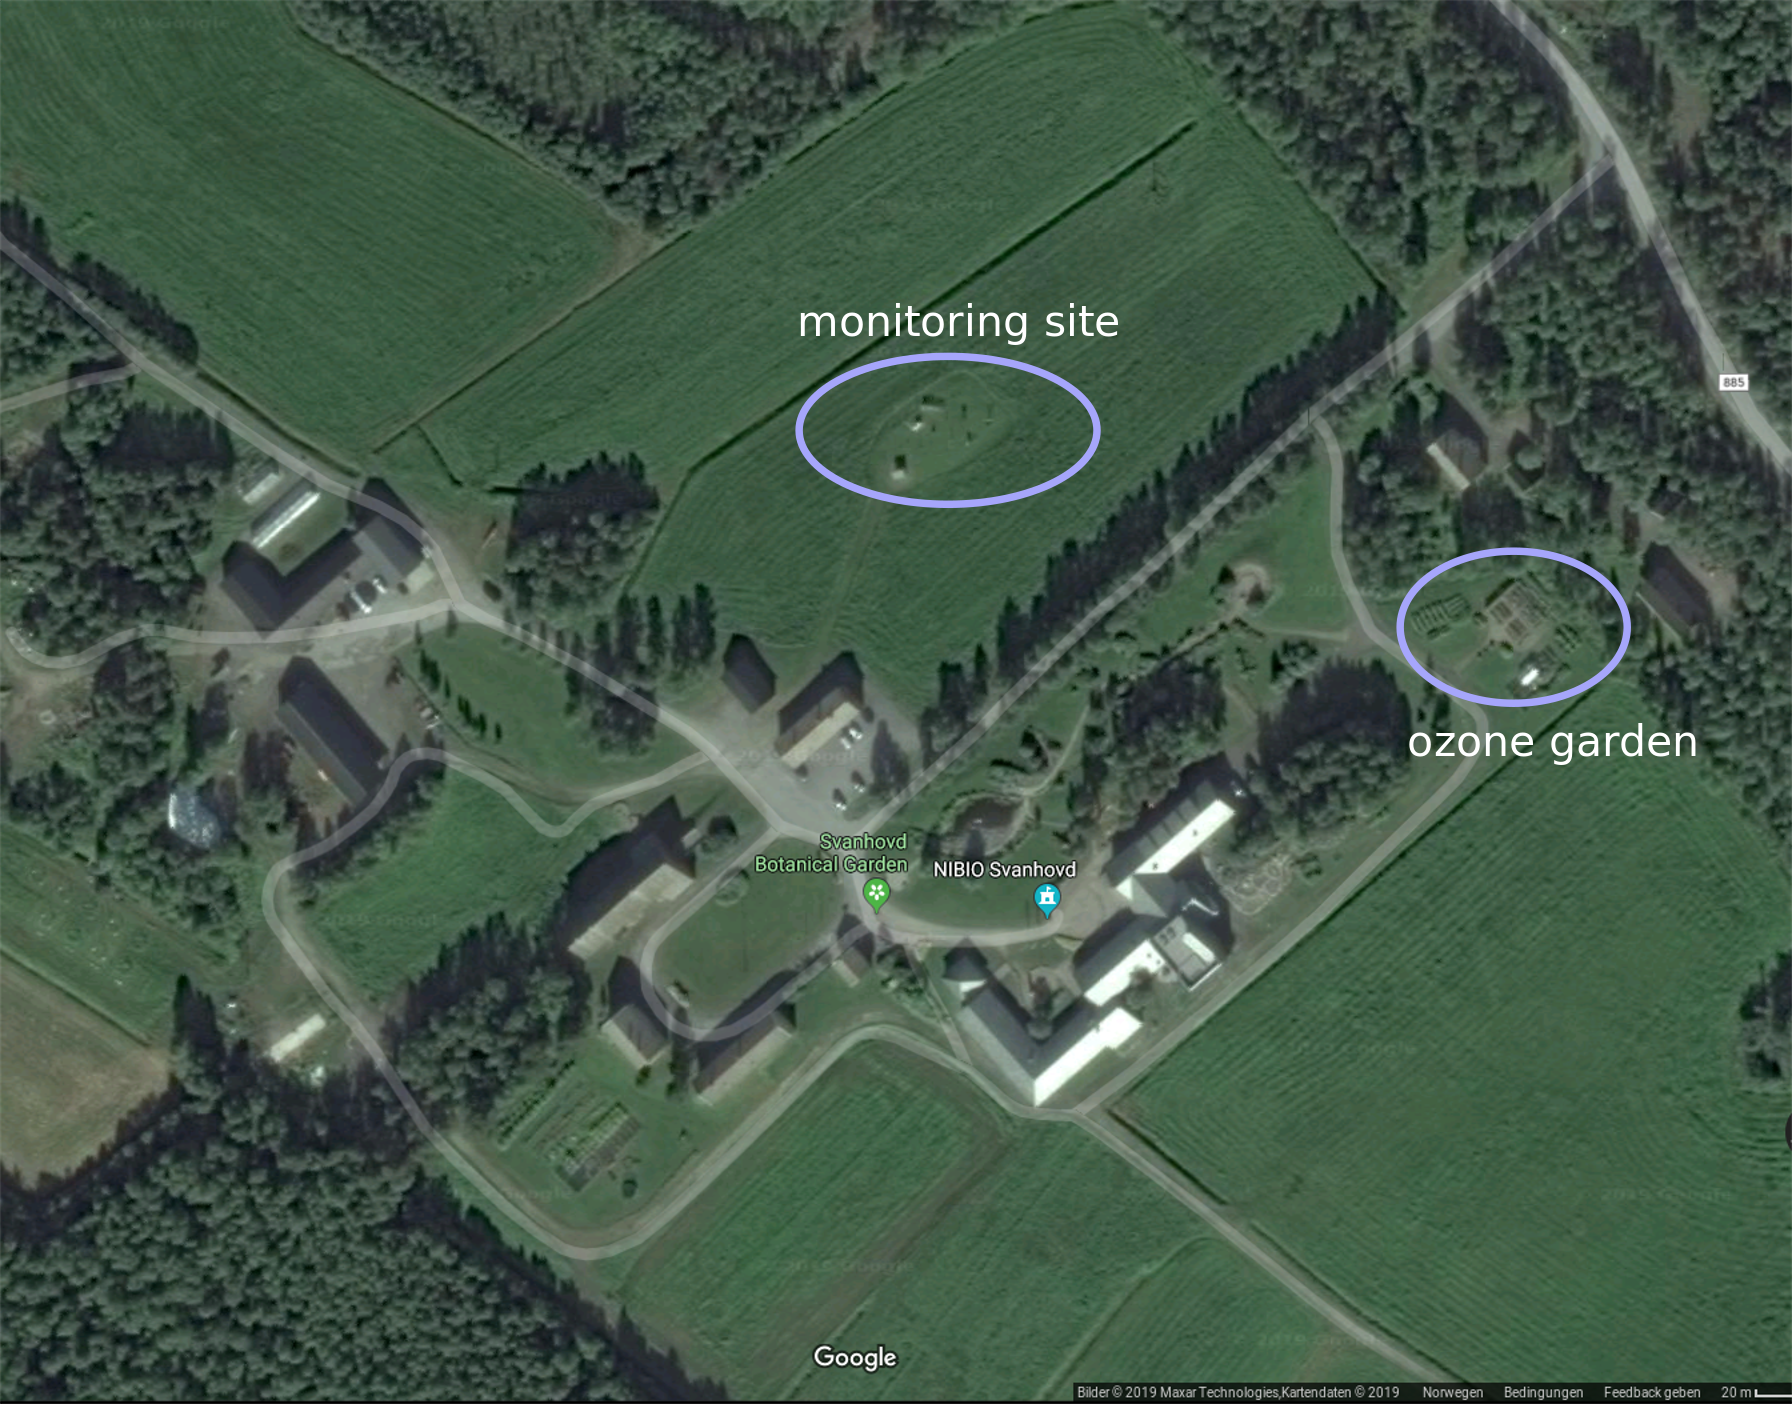
\includegraphics[width=8.3cm]{svanhovd_researchstation}\\
  %\includegraphics[width=8.3cm]{IMG_7739.JPG}
  \includegraphics[width=8.3cm]{fig01}
  \caption{NIBIO Environment Centre Svanhovd close by the settlement of Svanvik, Norway. (a) Atmospheric monitoring site and ozone garden have been marked. Aerial photography \copyright Norges Kartverk; (b) Clover in the Svanhovd ozone garden. The plants had to be secured against herbivores with a wire-mesh fence. The plants shown are approximately $6-12\,\unit{cm}$ high.}
  \label{fig:svanhovd_research_station}
\end{figure}


\subsection{2018/19 growing season}
\label{subsec:growing_season_1819}

All relevant data for the growing season 2018/19 are shown as timeseries in Fig.~\ref{fig:data_svanvik_2018_2019}. Ozone concentrations measured at $2\,\unit{m}$ height above ground are averaged hourly. The hatched areas mark times when no ozone data were recorded. Note, while the downtime during winter was planned, missing data in two weeks of July 2018 (July 9--23) were due to problems in data acquisition.

As can be seen in Fig.~\ref{fig:data_svanvik_2018_2019}a), \chem{[O_3]} peaks in spring (April/May) and reaches its minimum in late summer (July/August). The spring peak has not been captured completely in 2019, since data acquisition started later than in 2018. In summer 2018 (June--August), high ozone concentrations ($\chem{[O_3]} > 40\,\unit{ppb}$) were recorded 50 times. The highest summer ozone concentration ($\chem{[O_3]} = 50.2\,\unit{ppb}$) was measured on July 25. This coincides with the period of the most extensive forest fires in central Sweden which occurred from July 12--29 \citep{SOU2019}. However, due to the above-mentioned data acquisition problems, we missed most of the corresponding ozone data for this event and most likely also the peak \chem{[O_3]}. In contrast, \chem{[O_3]} only rose 18 times above the threshold of $40\,\unit{ppb}$ during the summer of 2019. For further analysis (Section~\ref{sec:stats}) and modeling study with the $\mathrm{DO_3SE}$ model (Section~\ref{sec:do3se}), we reconstructed the missing data. The used gap-filling method will be described in detail in a companion paper to be submitted.

Hourly averaged $2\,\unit{m}$ temperatures above $20\,\unit{^\circ C}$ occurred more regularly in July 2018 than in 2019 (Fig.~\ref{fig:data_svanvik_2018_2019}b). In 2018, spring temperature regularly rose above freezing only in May, while in 2019 this occurred already early in March/April.
More rain events with accumulated daily precipitation ($\sum_d \mathrm{Precip}$) above $10\,\unit{mm}$ occurred in the summer of 2018 compared to 2019 (Fig.~\ref{fig:data_svanvik_2018_2019}c).
Qualitatively, global irradiance ($Q_0$) displayed in Fig.~\ref{fig:data_svanvik_2018_2019}d) was higher in May and July 2018 compared to 2019, while June 2019 showed higher irradiance than 2018. A high global irradiance in most cases is the result of a low cloud fraction. In both years, the maximum recorded $Q_0$ was roughly $750\,\unit{W\,m^{-2}}$ reached in June as naturally expected.

\begin{figure*}[t]
  %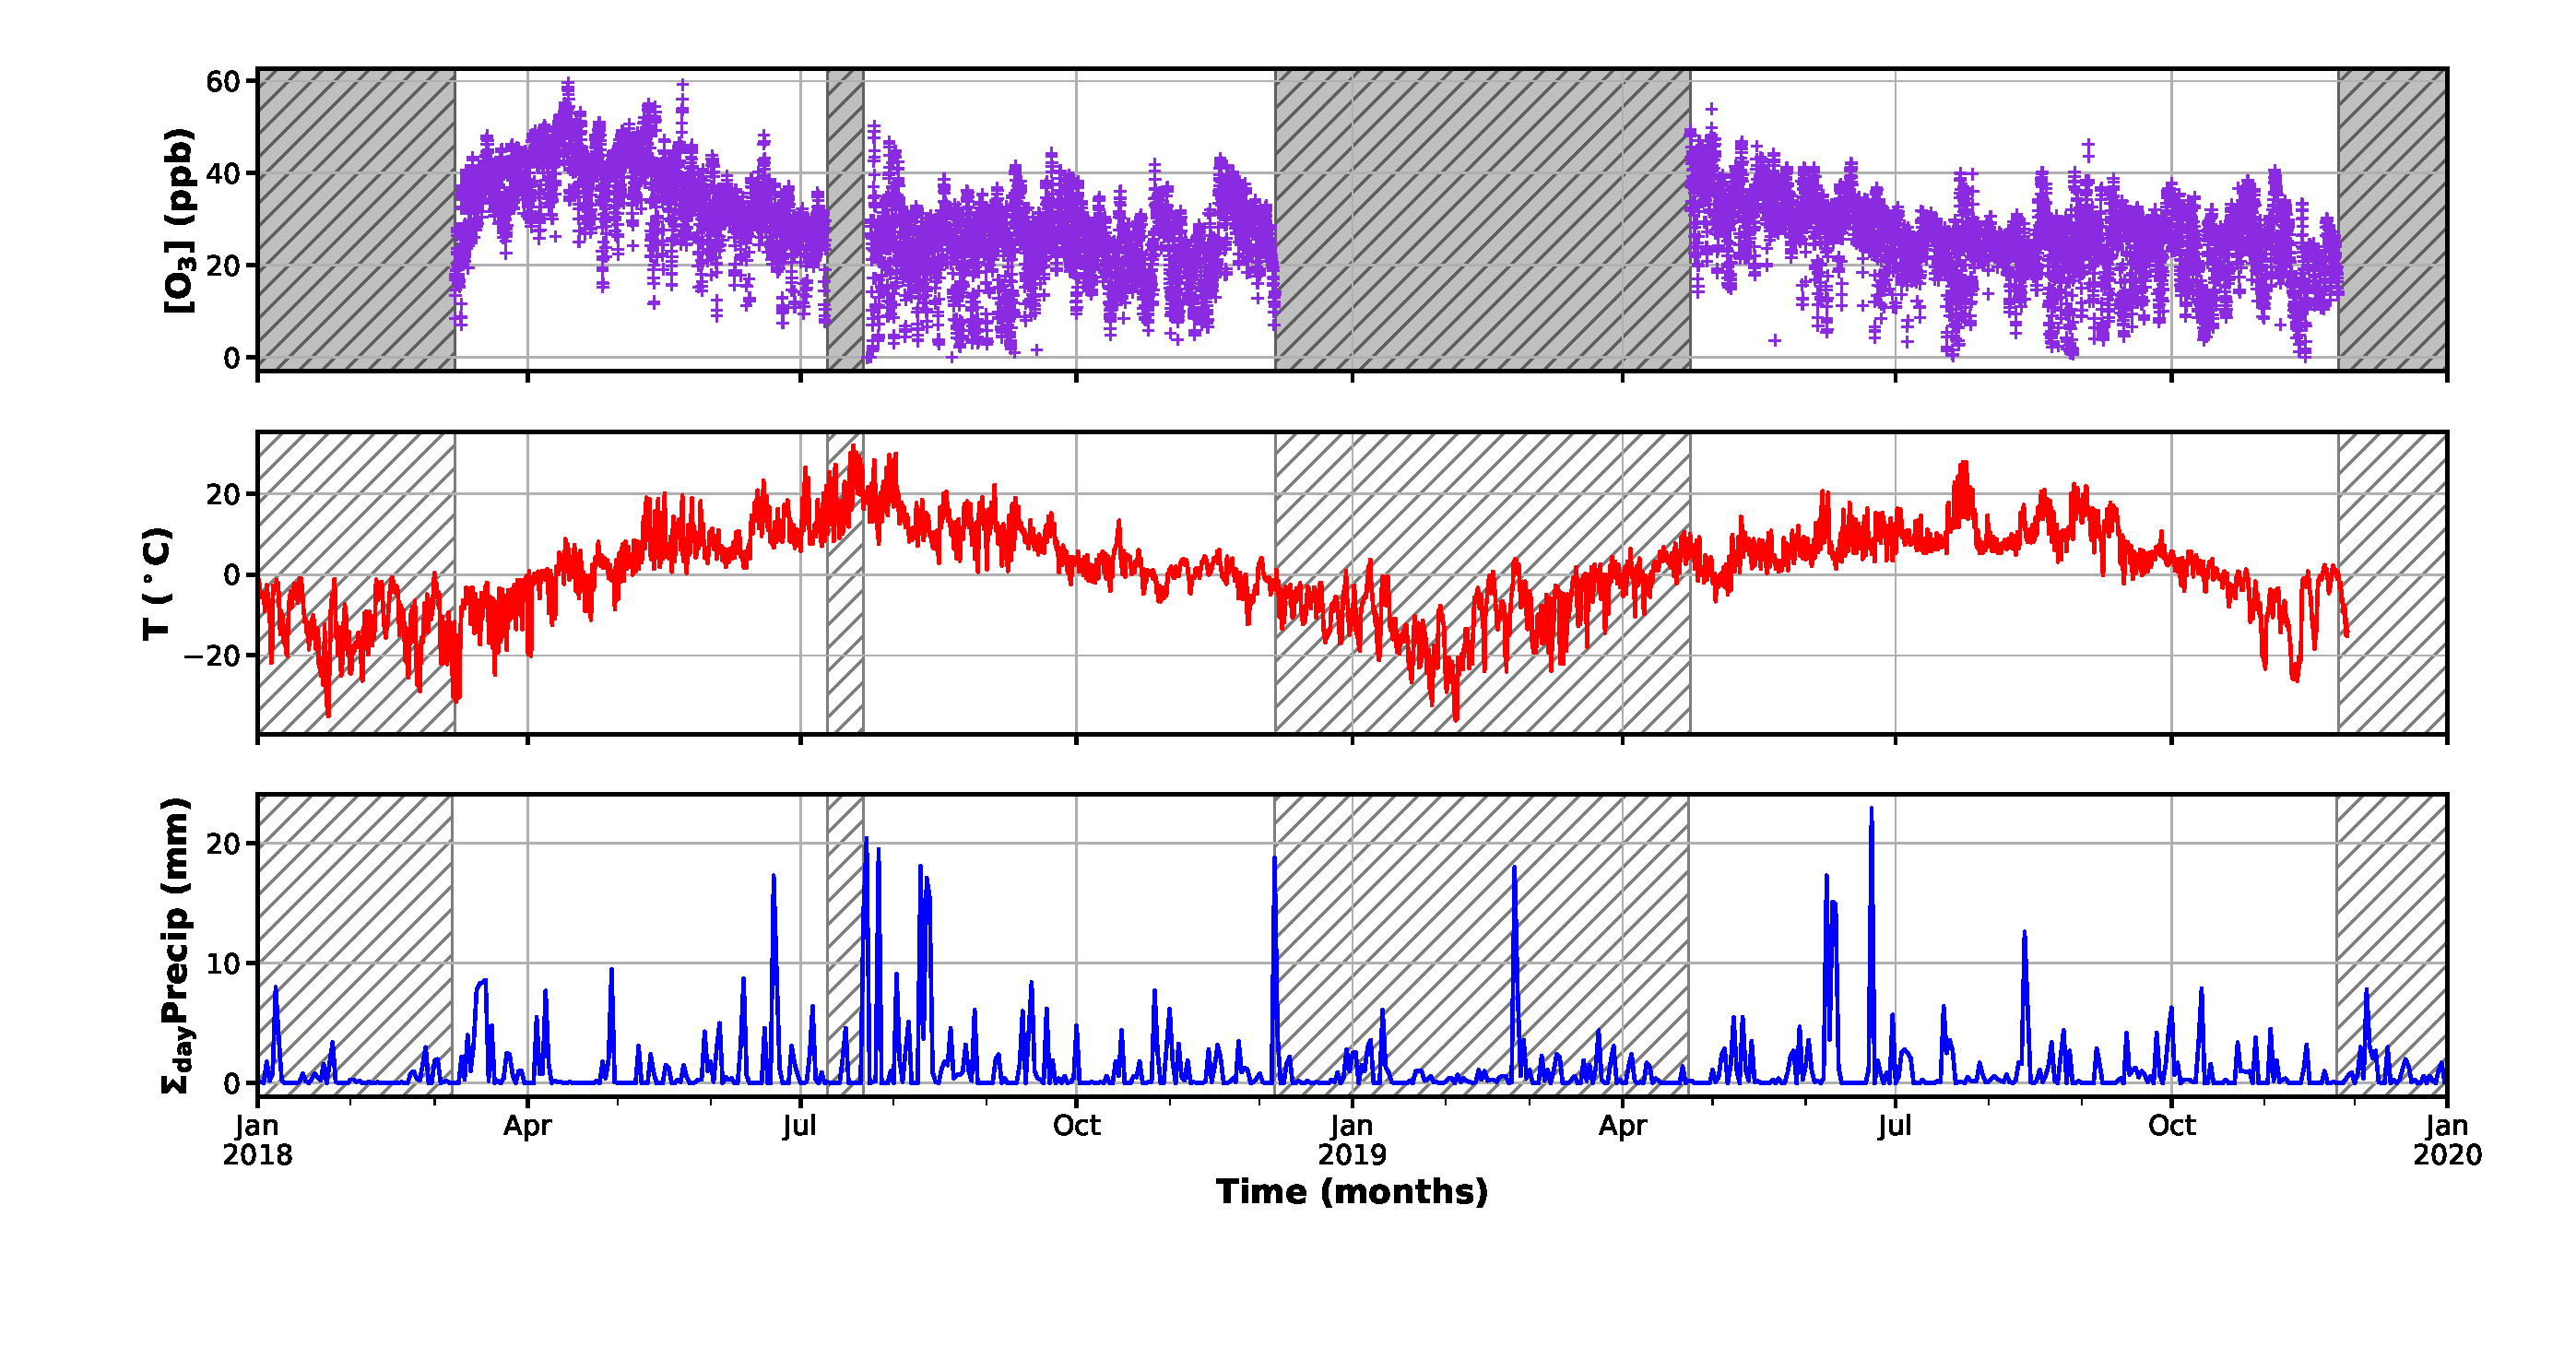
\includegraphics[width=12cm]{data_svanvik_2018_2019}
  \includegraphics[width=12cm]{fig02}
  \caption{Observational data from atmospheric monitoring at Svanhovd in 2018/19. The hatched areas indicate periods without ozone monitoring data. (a) Hourly averaged \chem{[O_3]}; (b) hourly averaged temperature; (c) daily accumulated precipitation; (d) hourly averaged global irradiance.}
  \label{fig:data_svanvik_2018_2019}
\end{figure*}

\subsection{Ozone data}
\label{subsec:ozone_data}
To determine the significance of the higher \chem{[O_3]} in 2018 in relation to regional averages and trends, we derive a ground-level \chem{[O_3]} climatology for Svanvik (Section~\ref{sec:stats}). From 1986--1996, ozone monitoring has been operated continuously by NILU at Svanhovd, but no ozone measurements have been conducted before the 2018/19 growing season. Due to probable changes in northern hemispheric tropospheric background ozone and a reduction of summertime peak values related to ozone precursors which fell under air quality regulations in Europe, we cross-calibrate our data with long-term ozone observations at sites in northern Finland and Sweden. 

%\subsubsection{Ground-level ozone observations}
%\label{subsubsec:ebas}
\begin{figure}[t]
  %\includegraphics[width=8.3cm]{station_map_fennoscandia}
  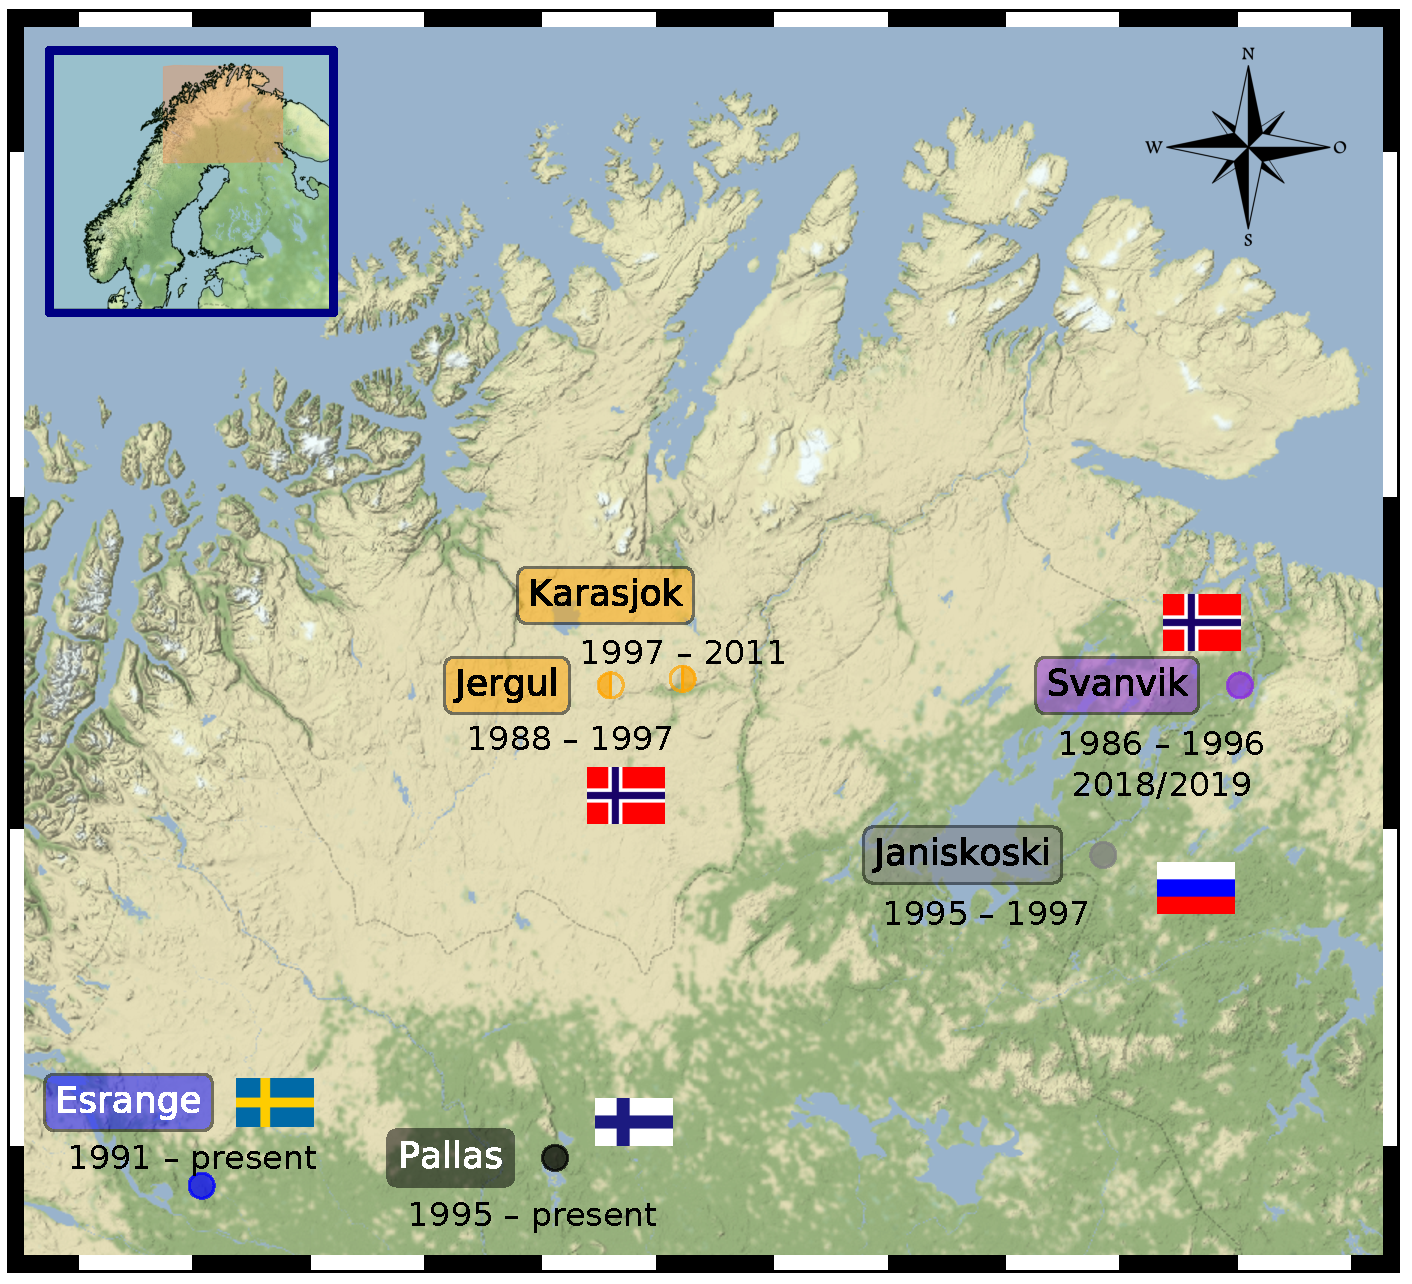
\includegraphics[width=8.3cm]{fig03}
  \caption{Cap of the North. Locations of past and present (end of 2018) ozone observation sites in northern Fennoscandia were used in this study. For more details see Tab.~\ref{tab:ebas_obs}. The same color coding for each station as displayed herein will be used in all the following figures.}
  \label{fig:station_map_fennoscandia}
\end{figure}


As indicated above, all ground-level ozone observations used in this study are available from the EBAS database operated by \citet{NILU_EBAS}. A comprehensive overview over all past and present ozone observation sites in northern Fennoscandia is given in Table~\ref{tab:ebas_obs} and Fig.~\ref{fig:station_map_fennoscandia}, respectively. All stations with available long-term observations are located at higher altitude than Svanhovd which will result in relatively higher ground-level \chem{[O_3]} in comparison. In the absence of local precursors, this is due to the stratification of the atmosphere leading to an increase in ozone abundance with altitude \citep[e.g.,][]{AB:Klingberg2009}. The periphery vegetation at all sites is similar and consists mainly of pine forests, birch, and heath. However, at higher spatial resolution the vegetation varies substantially. Ozone measurements at Pallas are taken on top of mount Sammaltunturi $100\,\unit{m}$ above treeline (pine forest) and the surrounding vegetation mainly consists of low vascular plants, mosses, and lichen \citep{BER:Hatakka2003}. At Svanhovd, the ozone measurements are taken amidst a meadow surrounded by agriculturally managed herbaceous plants and grass adhering to the \citet{WMOGuide2018} standards (Fig.\ref{fig:svanhovd_research_station}).

Data from before the 1990s are available solely from Svanvik and Karasjok. These data, however, do not follow the high-quality standard procedures implemented nowadays and have to be treated with care \citep{NILU2003}. Especially, ozone monitors did not undergo regular re-calibration. This probably leads to drifts in the observed data and may impose a false periodicity. In 1997, the ozone monitoring at Jergul was relocated downstream of the river Karasjokka to a site close by Karasjok. Although the same equipment has been used, this might have introduced a breaking point in the combined data series, denoted as Jergul/Karasjok in the following, which would be particularly problematic if these were the sole data for comparison. Only a few data have been taken upstream the Pasvik river at Janiskovski, hence these will not be taken into further consideration, but are shown for completeness. As can be seen in Fig.~\ref{fig:ozone_timesseries_fenoscandic_obs}, there is an overlap of about $4\,\unit{years}$ between data taken at Esrange, Jergul/Karasjok, and Svanvik. The hatched areas indicate periods with insufficient quality control as mentioned above.

\begin{table}[t]
  \caption{Past and present ozone observation sites in northern Fennoscandia. Data available on \href{http://ebas.nilu.no/}{EBAS}.}
  \label{tab:ebas_obs}
  \begin{tabular}{lllllrl}
    \tophline
    Name       & Country & ID      & \multicolumn{3}{c}{Location} & Operational\\
    &         &         & lat             & lon               & alt            &\\
    &         &         & (\unit{^\circ N}) & (\unit{^\circ E})  & (\unit{m})     &\\
    \middlehline
    Esrange    & SWE     & SE0013R & 67.83           & 21.07             & 475            & 1991 -- 2018$^1$\\
    Janiskoski & RUS     & RU0001R & 68.93           & 28.85             & 118            & 1995 -- 1997\\
    Jergul     & NOR     & NO0030R & 69.45           & 24.60             & 255            & 1997 -- 2011\\
    Karasjok   & NOR     & NO0055R & 69.467          & 25.217            & 333            & 1988 -- 1997\\
    Pallas     & FIN     & FI0096G & 67.97           & 24.12             & 565            & 1995 -- present$^2$\\
    Svanvik    & NOR     & NO0047R & 69.45           & 30.03             & 30             & 1986 -- 1996$^3$\\
    \bottomhline
  \end{tabular}
  \belowtable{$^1$ Data available on EBAS until the end of 2018.\\
    $^2$ Data available on EBAS until the end of 2019.\\
    $^3$ Exclusive ozone monitoring in growing seasons 2018/19 for the present study operated by NILU.} % Table Footnotes
\end{table}

\begin{figure*}[t]
  %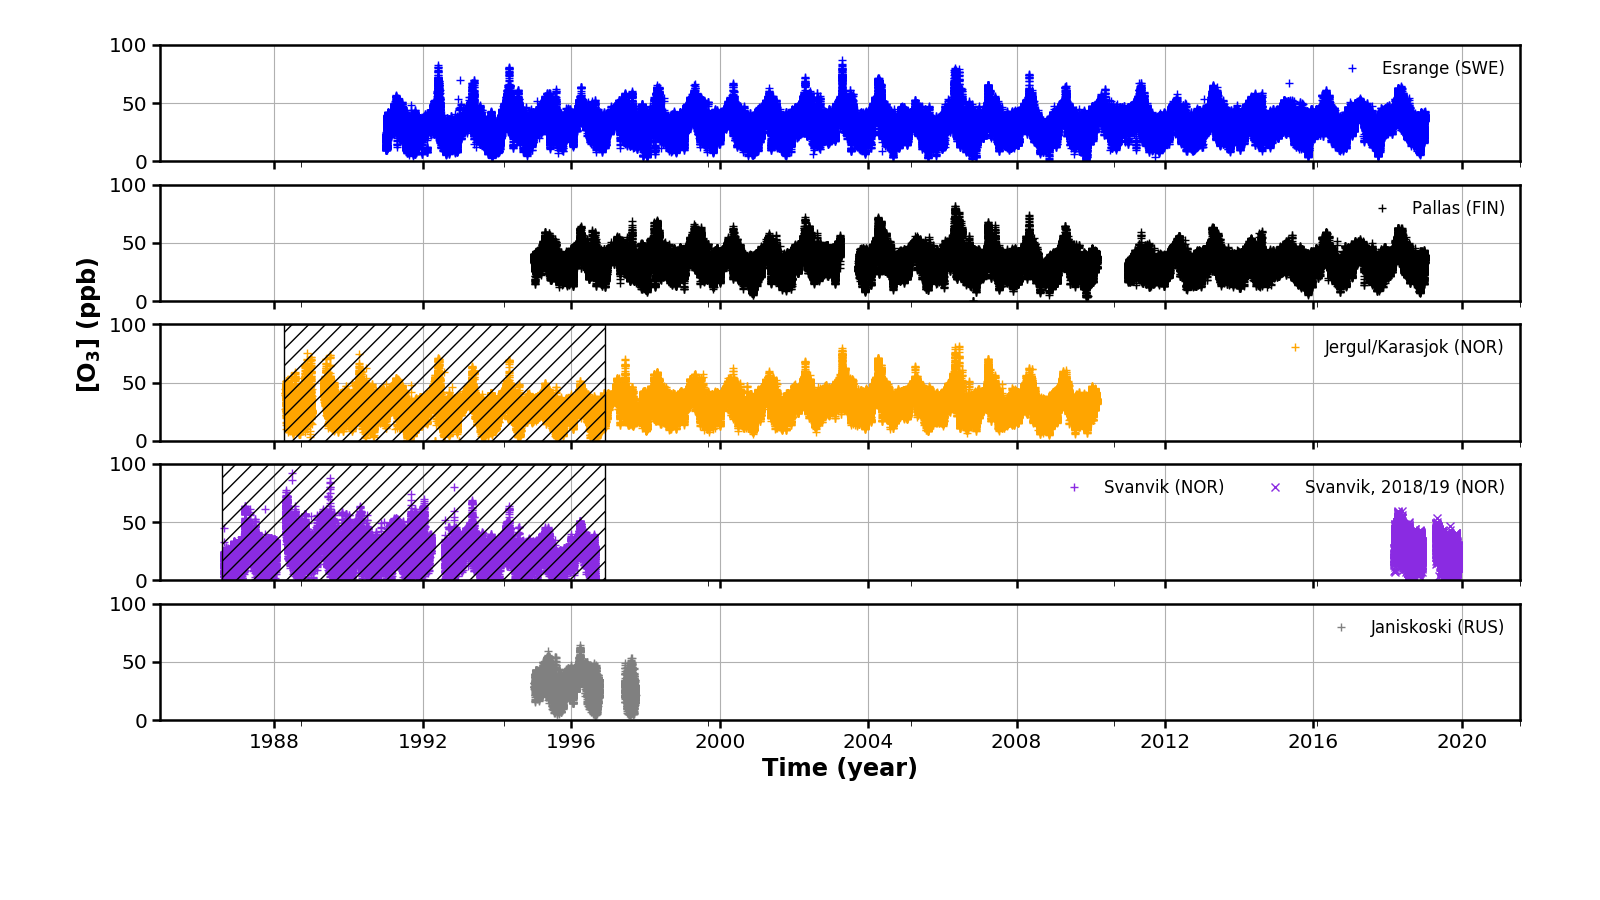
\includegraphics[width=12cm]{ozone_timeseries_fenoscandic_obs.png}
  \includegraphics[width=12cm]{fig04}
  \caption{Time series of ozone observations in northern Fennoscandia (Tab.~\ref{tab:ebas_obs}) (1986--2019). Data from EBAS until December 2018. The hatched areas indicate periods with insufficient quality control according to \citet{NILU2003}. (a) Esrange (SWE); (b) Pallas (FIN); (c) Jergul/Karasjok; (d) Svanvik; (e) Janiskoski.}
  \label{fig:ozone_timesseries_fenoscandic_obs}
\end{figure*}


\section{Statistical analysis}
\label{sec:stats}
In this section, we assess the climate conditions and multi-annual mean (referred to as climatology in thhe following) annual cycle of gound-level ozone concentrations at Svanhovd. To this end, we derive climatologies for temperature, precipitation, global irradiance, and ozone. We evaluate statistical significance of divergances from the norm in these variables for the growing seasons 2018/19 (referred to as anomalies). We perform a bias correction on the Svanvik ozone climatology with respect to long-term series of \chem{[O_3]} at the sites in northern Finland and Sweden.

\subsection{Derived climatologies}
\label{subsec:climatologies}

\subsubsection{Temperature, precipitation, and global irradiance}
\label{subsubsec:clim_temp_prec}
The location of Svanvik at $69.45\,\unit{^\circ N}$ suggests a subarctic climate. The derived climate diagram following Walter and Lieth which is shown in Fig.~\ref{fig:climatediagram} supports this very well. The diagram is based on climatological data from the atmospheric monitoring in Svanvik (1992--2012). Monthly averaged $2\,\unit{m}$ temperatures (red line) are displayed with a standard error of the mean (SE) as error band. We chose SE in this case due to the large interannual variability in temperature reflected in the standard deviation. Averaged monthly accumulated precipitation (blue bars) is shown with standard deviation of mean as error bars. Months with average temperatures below freezing are denoted with a star. As can be seen, temperatures stay below freezing for 5 consecutive months, while only 2 months breach $10\,\unit{^\circ C}$ regularly (July, August), satisfying the conditions for K\"{o}ppens climate classification of a regular subarctic climate (Dfc) \citep{SD:Beck2018}. The highest monthly average temperature is $(13.1\pm 1.1)\,\unit{^\circ C}$ in July and the lowest $(-12.8\pm 2.0)\,\unit{^\circ C}$ in February. In the period 1992--2012, the coldest measured temperature was $-45.2\,\unit{^\circ C}$ observed January 27, 1999, while the highest temperature on July 16 the same year was $29.4\,\unit{^\circ C}$.

\begin{figure}[t]
  %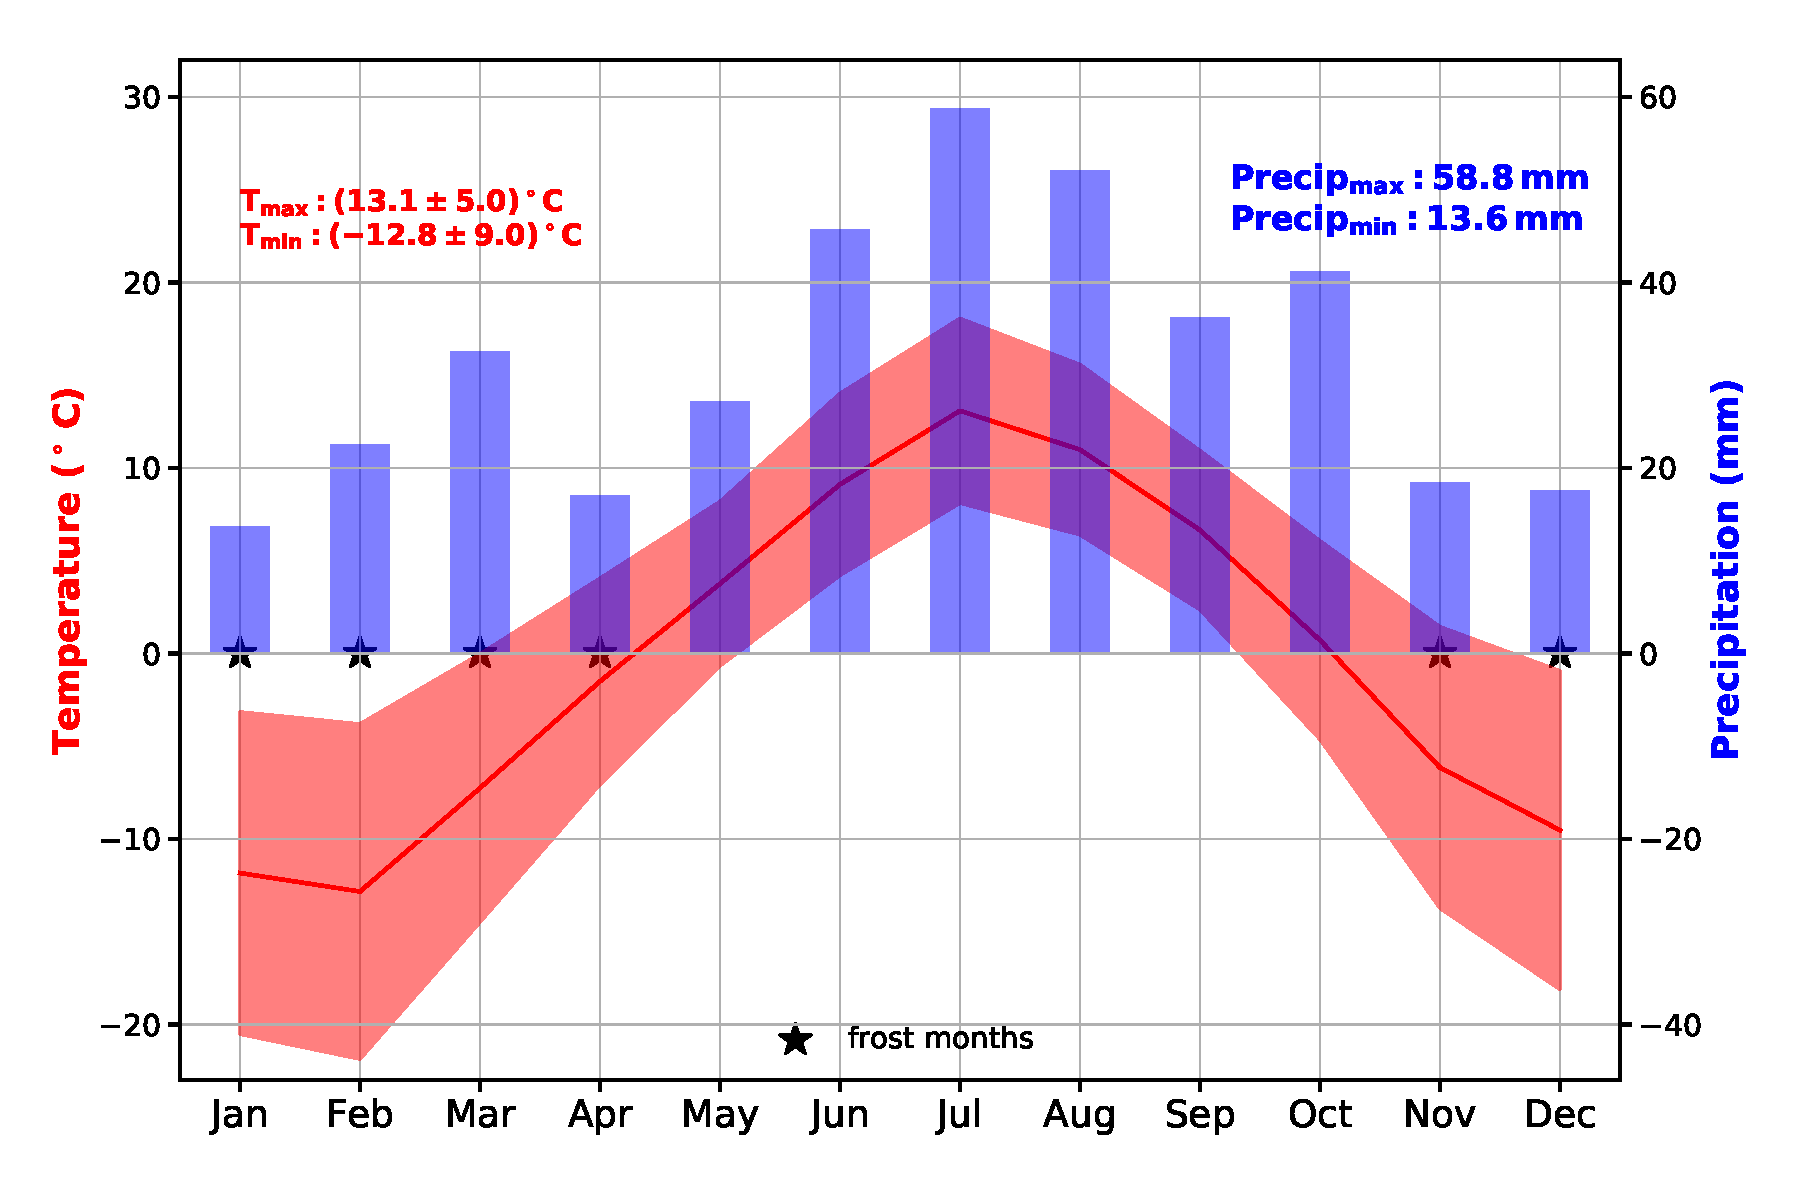
\includegraphics[width=8.3cm]{climatediagram}
  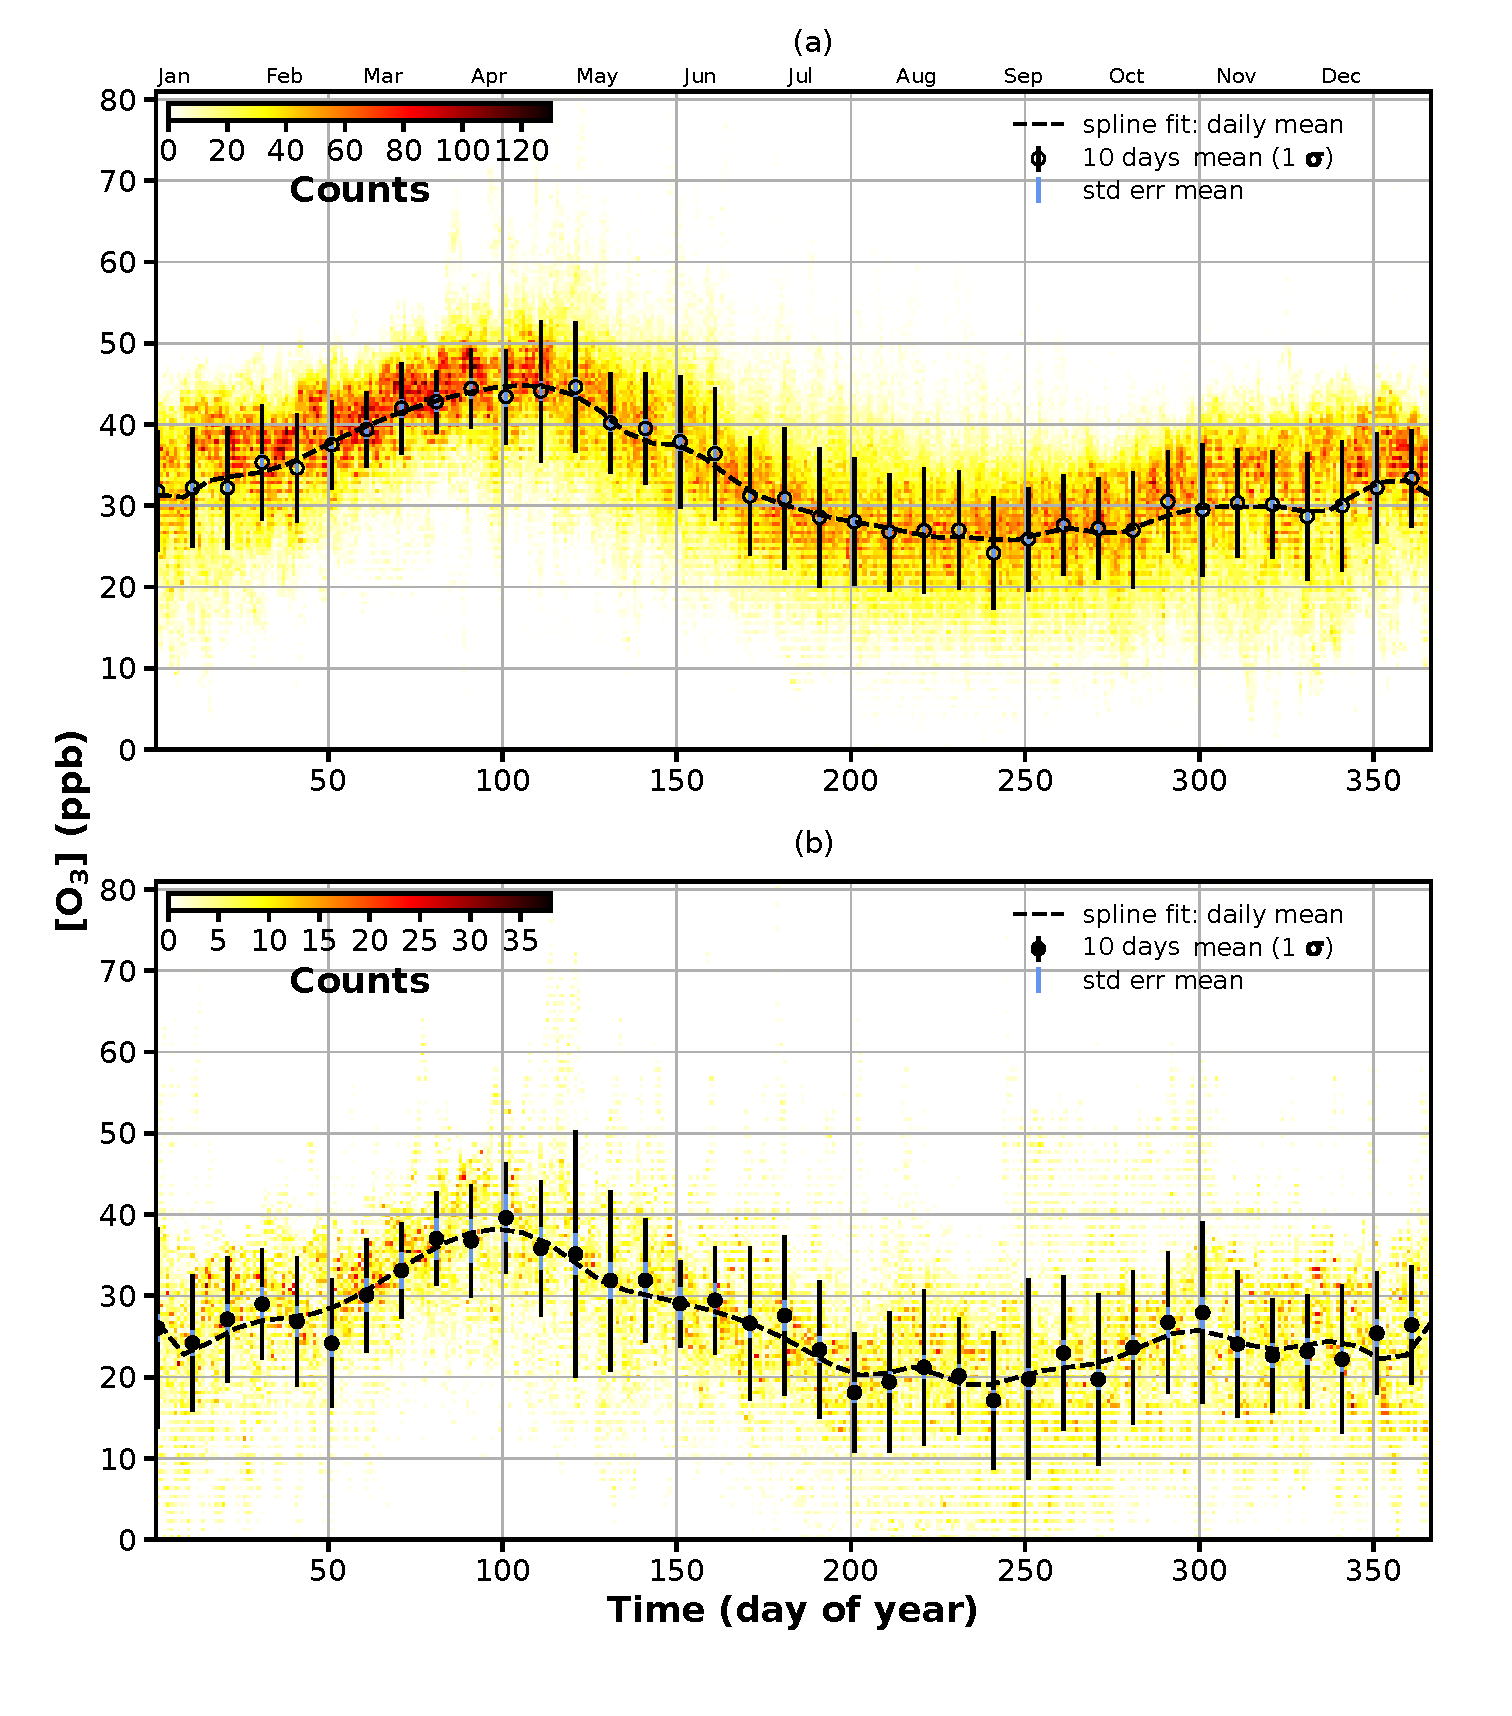
\includegraphics[width=8.3cm]{fig05}
  \caption{Climate diagram following Walter and Lieth. The diagram is based on climatological data for Svanvik/Pasvik (1992--2012) downloaded from LandbruksMeteorologiske Tjeneste. Monthly averaged temperatures (red line) are displayed with standard error of the mean as error band. Averaged monthly accumulated precipitation (blue bars) is shown with a standard deviation of mean as error bars. Months with average temperatures below freezing are denoted with a star.}
  \label{fig:climatediagram}
\end{figure}

The average accumulated monthly precipitation $\sum_d\mathrm{Precip}$ indicates that winter and spring (November--April, except for March) are relatively dry ($\sum_d\mathrm{Precip} < 20\,\unit{mm}$). The driest month is January with $\sum_d\mathrm{Precip} = (16.7\pm 3.0)\,\unit{mm}$. The most precipitation occurs in the summer months, with a $\sum\mathrm{Precip}_d = (58.5\pm 9.2)\,\unit{mm}$ in August. The average annual accumulated precipitation ($\sum_m\mathrm{Precip}$) given with standard error of mean is $(383\pm 86)\,\unit{mm}$. Precipitation shows a large interannual variability.

The derived climatology for global irradiance ($Q_0$) at Svanvik is shown in Appendix Fig.~\ref{fig:global_rad_clim}a). Shown are the average of hourly maximum $\left<Q_0^\mathrm{max}\right>$, minimum $\left<Q_0^\mathrm{min}\right>$, and mean $\left<Q_0^\mathrm{mean}\right>$. In agreement with the geometrically derived sunshine duration displayed in Supplement Fig.~\ref{fig:sunlight_fennoscandia}, $\left<Q_0^\mathrm{max}\right>$ approaches zero in December/January commonly known as polar night and reaches its maximum in June/July commonly referred to as midnight sun conditions. The highest observed $\left<Q_0^\mathrm{max}\right>$ is about $800\,\unit{W\,m^{-2}}$, while on average $\left<Q_0^\mathrm{mean}\right>$ it is about $450\,\unit{W\,m^{-2}}$ (regularly reached in May--July). The maximum of the climatological minimum $\left<Q_0^\mathrm{min}\right>$ lies at about $200\,\unit{W\,m^{-2}}$.


\subsubsection{Ozone}
\label{subsubsec:clim_ozone}
In the following, we will look at derived ozone climatologies from different perspectives.
The multi-annual means of daily mean ozone, for simplicity here without standard deviations, at observation sites in northern Fennoscandia (refer to Table~\ref{tab:ebas_obs} for details) are shown in Supplement Fig.~\ref{fig:ozone_climatology_fenoscandic_obs}. All climatologies except for Svanvik show peak values of about $48\,\unit{ppb}$ in late April. The spring peak values at Svanvik are lower because of the much lower altitude compared to the other monitoring sites. The annual average \chem{[O_3]} \chem{\left<[O_3]\right>} declines throughout the growing season until it reaches its minimum in late summer/fall ($24-30\,\unit{ppb}$). The turning points lie approximately in June and November. At Svanvik, \chem{\left<[O_3]\right>} is $6.6\,\unit{ppb}$ lower than on sites at Jergul/Karasjok (NOR), Esrange (SWE), and Pallas (FIN). The large spread in the case of Svanvik and Janiskoski is due to the lower number of observations.

The correlation of \chem{[O_3]} between Esrange, Pallas, and Jergul/Karasjok is fairly high ($r^2\approx 0.8$, Appendix Fig.~\ref{fig:density_distribution}a, b), hence we can put those data series together to derive a general ozone climatology for northern Fennoscandia. The correlation between Svanvik and Esrange and Pallas is rather low, 0.4 and 0.6, respectively. Thus, Svanvik cannot directly be represented by any measurements taken at either Esrange or Pallas. We shall come back to this in Section~\ref{subsec:ozone_reco}.

In Figure~\ref{fig:ozone_climatology_fenoscandic_obs_spline}, the two dimensional density distributions of \chem{[O_3]} for the combined northern Fennoscandia data (Fig.~\ref{fig:ozone_climatology_fenoscandic_obs_spline}a) and Svanvik (Fig.~\ref{fig:ozone_climatology_fenoscandic_obs_spline}b) are shown. Darker colors indicate higher probability to observe these values. On top of the density distributions, $10\,\unit{days}$ averages of daily mean \chem{\left<[O_3]\right>_\mathrm{10\,\unit{d}}} are displayed together with $1 \sigma$ uncertainties and SE, respectively. Splines have been fitted through the data for easier inter-comparison with reanalysis data.
From the northern Fennoscandia climatology, one can deduce several features. The build-up of the ozone spring peak takes about $7.5\,\unit{months}$ from minimum to maximum. A sharp increase starts one month ahead of the estimated begin of greening $G_\mathrm{begin}$ (see Section~\ref{subsec:do3se_parameters} for details) and is in coincident with rising temperatures and global irradiance. We find day of the year (\unit{doy}) $\left<G_\mathrm{begin}\right> = (150 \pm 14)$ for Svanvik (Supplement Fig~\ref{fig:greening_season_change_Svanvik}), which translates to the end of May. This finding is in line with more extensive studies \citep[][e.g.,]{IJB:Karlsen2007,AFM:Linderholm2006}. The maximum of \chem{\left<[O_3]\right>_\mathrm{10\,\unit{d}}} is reached in late April ($100-120\,\unit{doy}$). The depletion of ozone from maximum to minimum takes only $4.5\,\unit{months}$. The minimum occurs at $25\,\unit{ppb}$ in the beginning of September ($240-250\,\unit{doy}$).

The density distribution for Svanvik and the \chem{\left<[O_3]\right>_\mathrm{10\,\unit{d}}} display a similar pattern as the northern Fennoscandia climatology (Fig.~\ref{fig:ozone_climatology_fenoscandic_obs_spline}b). The spring peak occurs slightly earlier (at the beginning of April). As Svanvik is located at a lower altitude than the other sites, the earlier decline of the ozone peak may point to a stronger influence of vegetation on the removal of ozone. \chem{CO_2} uptake by coniferous trees can occur as early as \unit{doy} 100 \citep{TB:Kolari2007, TP:Wallin2013}. The average \chem{[O_3]} at Svanvik is lower than at the other sites, as already mentioned, which is in league with a decrease in tropospheric ozone with decreasing altitude. In July--September, ozone is occasionally almost completely depleted during nighttime.

\begin{figure}[t]
  %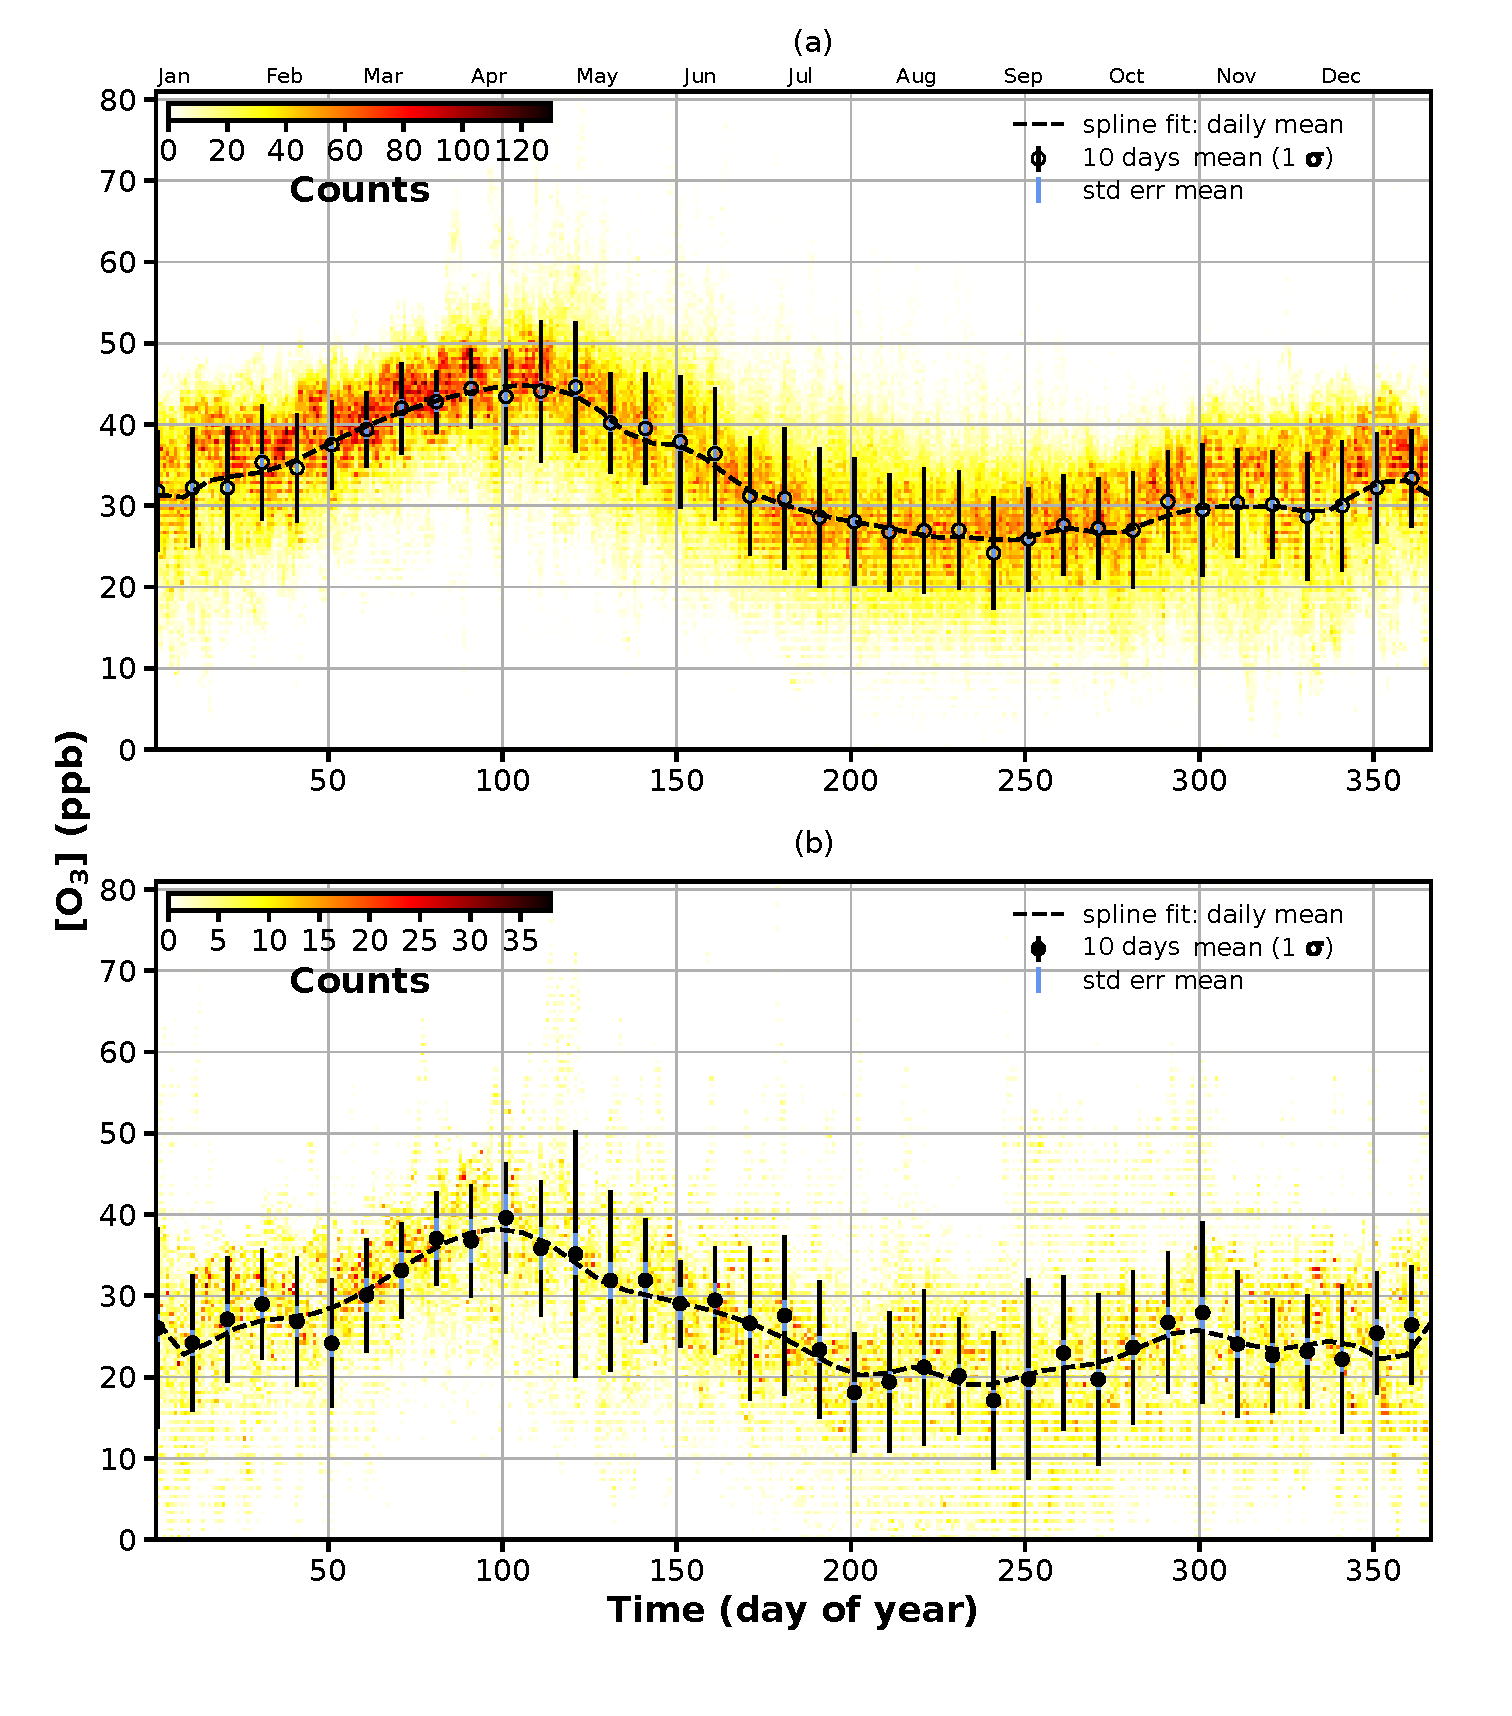
\includegraphics[width=8.3cm]{ozone_climatology_fenoscandic_obs_spline}
  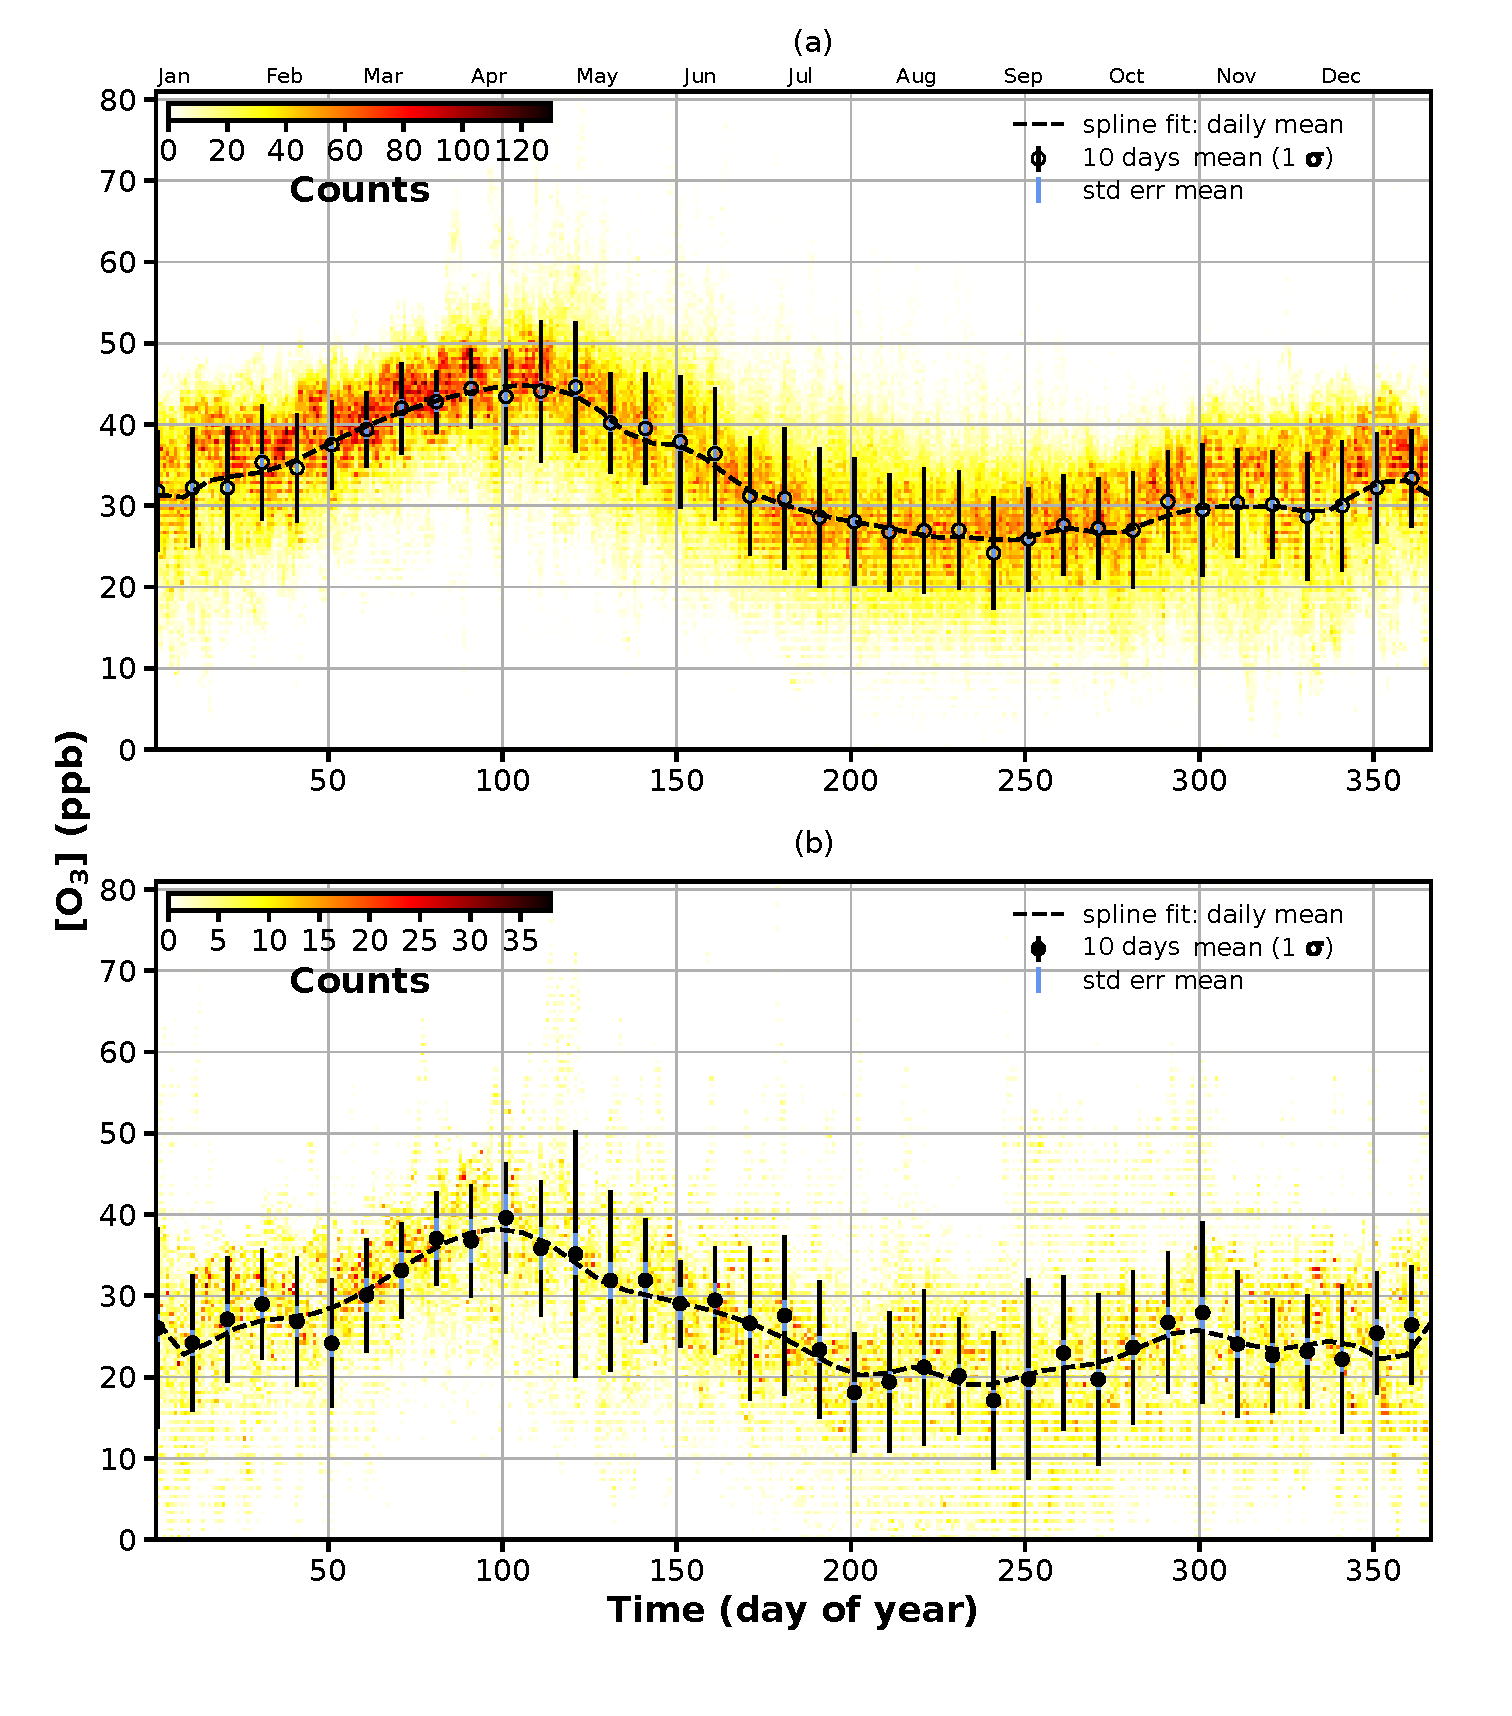
\includegraphics[width=8.3cm]{fig06}
  \caption{Ozone climatologies. Fennoscandia combines all available data from Jergul/Karasjok, Esrange, and Pallas. The density distributions are shown together with a multi-annual mean of daily \chem{[O_3]} (climatology). Splines have been fitted through daily mean \chem{[O_3]}. The climatology of daily mean ozone is shown together with $1\,\sigma$ standard deviation and standard error of the mean. Since \chem{[O_3]} are strongly correlated for sites at Jergul/Karasjok (NOR), Esrange (SWE), and Pallas (FIN) (see Fig.~\ref{fig:density_distribution}), data of these have been averaged together to derive a climatology for northern Fennoscandia. (a) Northern Fennoscandia; (b) Svanvik.}
  \label{fig:ozone_climatology_fenoscandic_obs_spline}
\end{figure}


\subsection{2018/19 anomalies}
\label{subsec:anomalies}
Using these established climatologies, we look at the anomalies in 2018/19 and discuss the differences between the two years. As weather extremes like in 2018 are likely to become more frequent with climate change, this will help to improve our understanding of a possible future increase in vulnerability of subarctic vegetation to ozone. 

\subsubsection{Temperature, precipitation, and global irradiance}
\label{subsubsec:anomal_tpq}
In Fig.~\ref{fig:anomalies_svanvik}a), temperature anomalies at Svanvik are shown as a percentage of days warmer or colder than $\pm 1\,\sigma$ from the climatological mean for each month. Negative deviations from climatology are displayed as a negative percentage. The full annual positive/negative deviations are indicated in the respective corners (right upper/right lower). The hatched area between the dashed lines indicates the expected percentage of values falling above/below $\pm 1\,\sigma$ if a normal distribution is assumed ($15.9\,\unit{\%}$). The summer of 2018 was significantly warmer than average. Especially in May and July more than $40\,\unit{\%}$ of the days were significantly warmer. Significantly warmer days continued to occur in all months (August--November) except for October. March 2018 had many unusually cold days. The summer of 2019 was fairly average, however, significantly colder days in July occurred, while August had both significantly colder and warmer days. April 2019 had significantly warmer than average days.

\begin{figure}[t]
  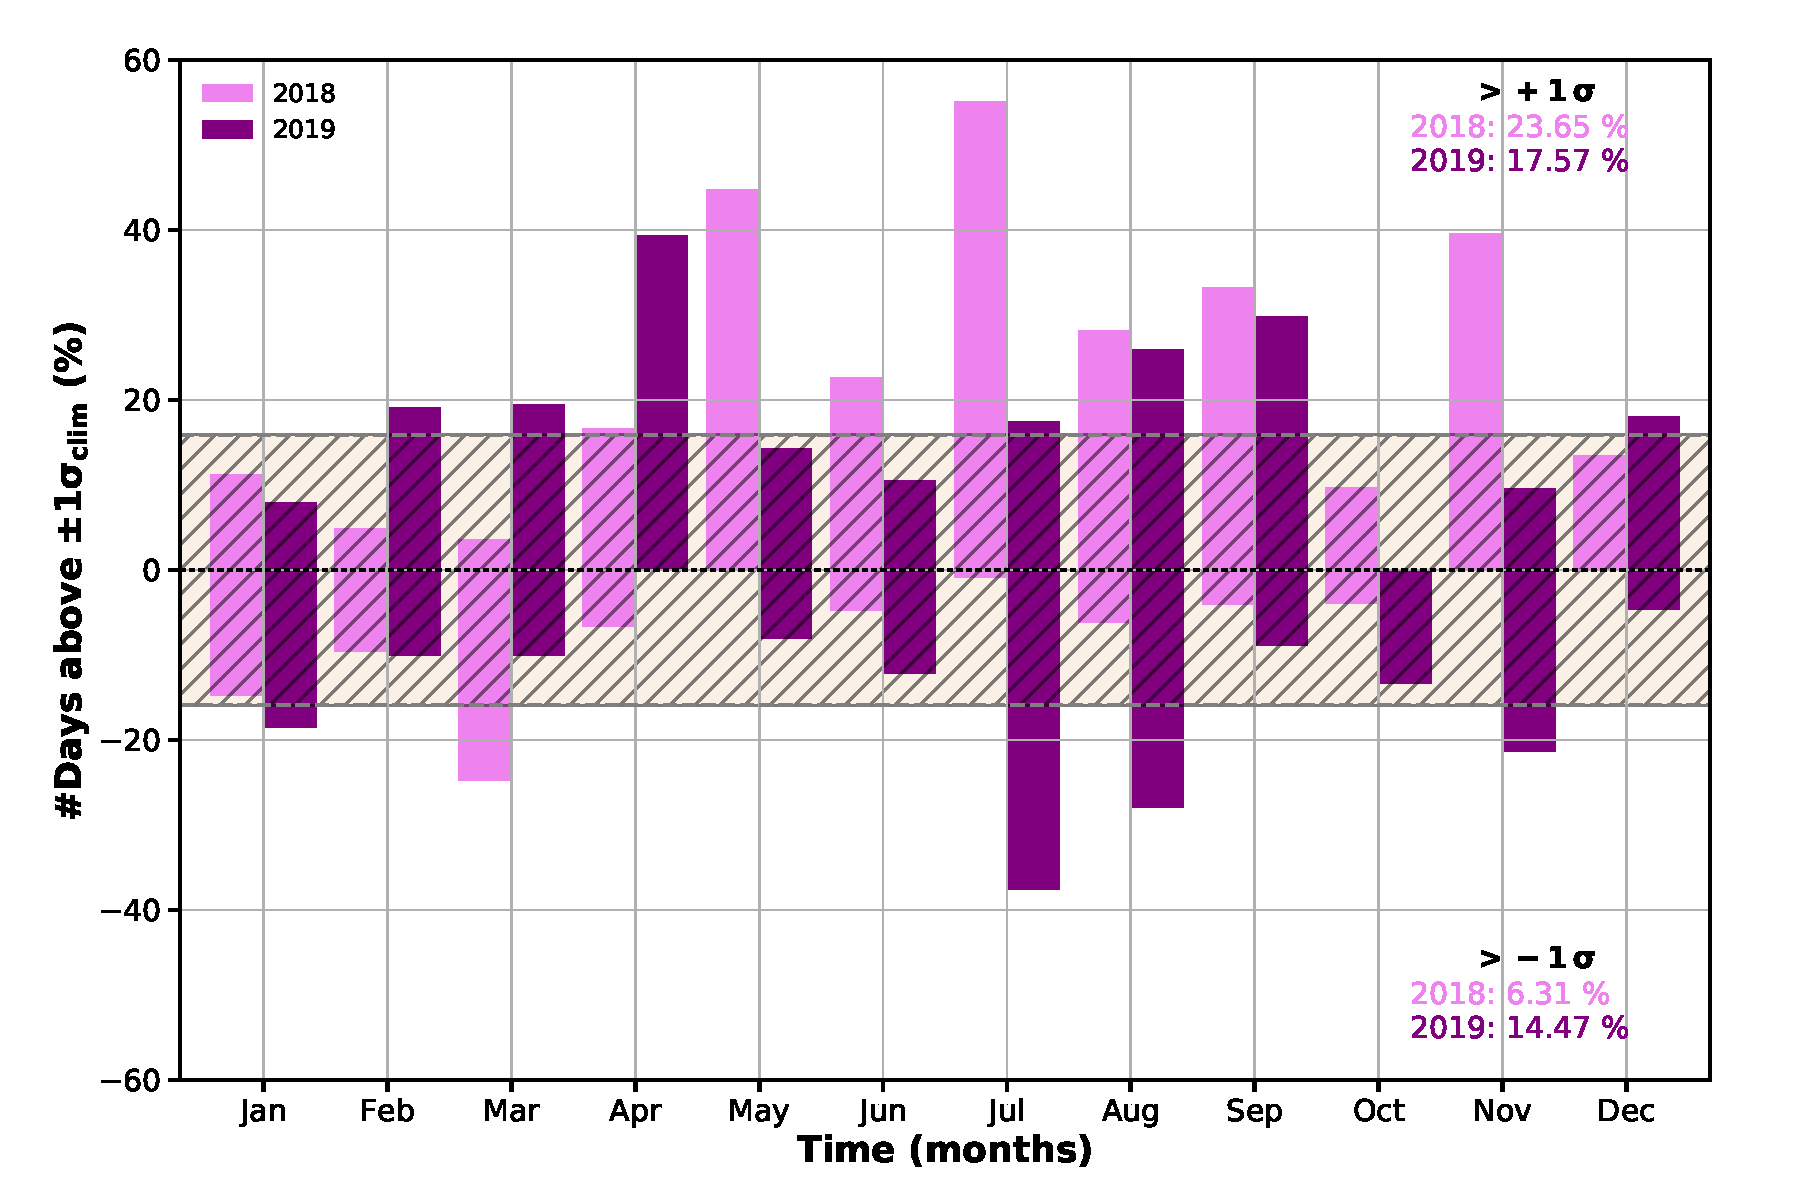
\includegraphics[width=12cm]{fig08}
  \caption{2018/19 anomalies of key environmental variables at Svanhovd displayed as percentages of days significantly deviating from climatological mean through standard deviation for each month. Negative deviations from the climatology are shown as a negative percentage. The annual positive/negative deviations are indicated in the respective corners (right upper/right lower). The hatched area between the dashed lines indicates statistical significance under the assumption of a normal distribution ($15.9\,\unit{\%}$, $30.8\,\unit{\%}$ for Precip.). (a) Temperature; (b) precipitation; (c) global irradiance; (d) ozone.}
  \label{fig:anomalies_svanvik}
\end{figure}

Similarly, the precipitation anomalies at Svanvik are displayed in Fig.~\ref{fig:anomalies_svanvik}b). Due to large interannual variability in observed precipitation, only a few days deviated significantly from the climatology on the $1 \sigma$ level. Therefore, we lowered the $\sigma$ level constraint. The percentage of days wetter/drier than $\pm \frac{1}{2}\,\sigma$ from the climatological mean are shown for each month. Negative deviations from the climatology are shown as a negative percentage and annual positive/negative deviations are indicated in the respective corners. The hatched area between the dashed lines indicates the expected percentage of values falling above $\pm\frac{1}{2}\,\sigma$ if a normal distribution is assumed ($30.8\,\unit{\%}$). Unlike the temperature anomalies, the picture is not as clear. While March 2018 had a significant number of days wetter than unusual, summer and fall (May/July, September/October) had a significant number of days drier than average. Overall, 2019 was rather average throughout the year, but with a significant number of days drier than normal (September/October) and a wetter December.

Similarly, the global irradiance anomalies at Svanvik are presented in Fig.~\ref{fig:anomalies_svanvik}c). The percentage of days above or below $\pm 1\,\sigma$ from the climatological mean is displayed for each month. The hatched area between the dashed lines indicates the expected percentage of values falling above/below $\pm 1\,\sigma$ if a normal distribution is assumed. In summer 2018 (May/July), global irradiance showed a significant number of days with higher than average irradiance, while 2019 was generally an average year with a significant number of days darker in spring (April/May).

In summary, 2018 had a significant number of days that were warmer, drier, and brighter than the climatological average, while 2019 was a rather average year.

\subsubsection{Ozone}
\label{subsubsec:anomal_ozone}
As we discussed in the preceding Section~\ref{subsubsec:anomal_tpq}, meteorological conditions in 2018 were significantly different from the climatological average. How does this translate into observed ozone anomalies \chem{\Delta[O_3]}?

If the data collected at Svanvik had been complete in 2018 and the climatology had extended into the recent past, we could have assessed the significance of ozone anomalies in the same way as for temperature, precipitation, and global irradiance. In Section~\ref{subsubsec:clim_ozone}, we described the construction of climatologies for northern Fennoscandia based on long-term observations at Esrange, Jergul/Karasjok, and Pallas. For Svanvik this assessment is based on rather uncertain observations from 1986--1996. We also discussed the general patterns, similarities, and differences. We shall now investigate \chem{\Delta[O_3]} in 2018/19 for these climatologies in more detail.

In the following, we will use the interchangeable terms anomalies and residuals to distinguish between a climatological (anomalies) and a statistical (residuals) point of view.
All the above factors make it necessary to look not only at anomalies but statistically also to assess ozone concentration residuals at Svanvik as well as at Esrange and Pallas in comparison. Since the climatology of the latter is more reliable, we will start with ground-level ozone concentration residuals \chem{\Delta[O_3]} at Esrange and Pallas in 2018. As data for 2019 has not yet been available from EBAS (last access, February 2020), we refrain from looking into these.

In Supplement Fig.~\ref{fig:ozone_climatology_fenoscandic_obs_residuals}, the probability density functions of daily mean ozone concentration residuals for Esrange and Pallas are shown. Both stations display a clear, but not significant, deviation from the climatological mean. On average, \chem{[O_3]} had been elevated by $(1.9\pm 5.7)\,\unit{ppb}$ and $(1.9\pm 5.4)\,\unit{ppb}$, respectively. Both distributions are slightly skewed towards positive deviations with $\frac{1}{4}$ of days (3. quantile, q3) falling above $5.8\,\unit{ppb}$ and $5.6\,\unit{ppb}$, respectively.

Supplement Figure~\ref{fig:ozone_climatology_fenoscandic_obs_residuals-Svanvik} displays the probability density functions of daily mean ozone concentration residuals for Svanvik based on data taken in 2018/19 with respect to the climatology derived for northern Fennoscandia (denoted NF in Supplement Fig.~\ref{fig:ozone_climatology_fenoscandic_obs_residuals-Svanvik}a) and the climatology derived for Svanvik (Supplement Fig.~\ref{fig:ozone_climatology_fenoscandic_obs_residuals-Svanvik}b).
As previously mentioned, \chem{\left<[O_3]\right>} at Svanvik are $(6.6\pm 7.1)\,\unit{ppb}$ lower than the northern Fennoscandia climatology. For 2018 and 2019, we find $\Delta\chem{\left<[O_3]\right>} = (-3.8\pm 5.6)\,\unit{ppb}$ and $\Delta\chem{\left<[O_3]\right>} = (-5.2\pm 5.0)\,\unit{ppb}$, respectively. While the probability density of the residuals between the two climatologies is skewed towards negative values, the skew of 2018/19 is positive.
With respect to the climatology for Svanvik (Supplement Fig.~\ref{fig:ozone_climatology_fenoscandic_obs_residuals-Svanvik}b), the probability density functions average for 2018/19 lies at $\Delta\chem{\left<[O_3]\right>} = (2.6\pm 5.8)\,\unit{ppb}$ and $\Delta\chem{\left<[O_3]\right>} = (1.2\pm 5.0)\,\unit{ppb}$, respectively.
Neither of the \chem{\Delta\left<[O_3]\right>} is significant by statistical means, but daily average ozone concentrations are slightly elevated in 2018 compared to 2019.

The \chem{\left<\Delta\left<[O_3]\right>\right>} for Svanvik in 2018 is slightly larger than for Esrange and Pallas. This could mean either that 2018 had been more exceptional at Svanvik or the derived climatology may need a correction for increased tropospheric background ozone concentration. Based on the meteorological conditions, we assume 2019 as an average year which leads to an estimated constant bias of about $1.2\,\unit{ppb}$ in \chem{[O_3]}. Daily \chem{\Delta_{present-past}\left<[O_3]\right>} from Esrange and Pallas, wherein present is defined as the average of 2010--2018 and past as the respective beginning of data taking until 1997, do not reveal a clear trend: We find for Esrange $(1.5\pm 3.1)\,\unit{ppb}$ and for Pallas $(-2.5\pm 3.7)\,\unit{ppb}$ \citep{NILU2003, BER:Ruoho-Airola2015}. Former is compatible with our assumed bias for the climatology derived for Svanvik.

To further investigate the ozone residuals, we conduct a Student's~t-test ($t = \frac{\chem{\Delta[O_3]}}{\sigma}$), assuming the same sample uncertainty $\sigma$ in both, climatology and the year in question. Results for Esrange and Pallas are shown in Supplement Fig.~\ref{fig:ozone_climatology_fenoscandic_obs_test}. This t-test clearly shows, that at both sites the residuals are significant on the $1\sigma$ level for at least $50\,\unit{\%}$. In Supplement Fig.~\ref{fig:ozone_climatology_fenoscandic_obs_test-Svanvik}, the test statistics for Svanvik are displayed. From Supplement Fig.~\ref{fig:ozone_climatology_fenoscandic_obs_test-Svanvik}a), we can deduce, that the residuals between the Svanvik climatology and the northern Fennoscandia climatology are significant on the $2\sigma$ level for at least half of the data, while the residuals are less certain in 2018 and 2019. In Supplement Fig.~\ref{fig:ozone_climatology_fenoscandic_obs_test-Svanvik}b) the same is shown for the years 2018/19 for the climatology from Svanvik. We find that less than $50\,\unit{\%}$ of ozone concentration residuals are significant on the $1\sigma$ level.

In accordance to the above findings, we adjust the derived ozone climatology for Svanvik by adding a constant bias correction factor $\Delta\chem{[O_3]_\mathrm{bias-corr}} = 1.2\,\unit{ppb}$ and estimate the ozone concentration anomalies for 2018/19. In Fig.~\ref{fig:anomalies_svanvik}d), the resulting percentage of days above/below $\pm 1\,\sigma$ from the bias-corrected climatological mean is displayed for each month. Negative deviations from climatology are shown as a negative percentage. Note that missing bars for certain months are both due to data availability (see Fig~\ref{fig:data_svanvik_2018_2019} for details concerning Svanvik) and anomalies not meeting the criteria of $\pm 1\sigma$ deviation from the climatological mean. In April/May 2018, ozone was significantly enhanced, while 2019 was generally an average year. In both years, ozone concentrations were significantly below average in November. July 2018 represented by the color bar has not been corrected for the missing data due to data acquisition problems. The corrected value is indicated by the star. A detailed describtion of the gap-filling based on a Reynolds's decomposition method will be published seperately.

To conclude, ozone concentrations in 2018 have been elevated compared to the respective climatologies, however, on average not significantly by statistical means. At Esrange and Pallas at least $25\,\unit{\%}$ (3.~quantile) of anomalies are significant on a $3\sigma$ level or more, while at Svanvik the 3.~quantile lies at about $2\sigma$. This means that in 2018 the stations at Esrange and Pallas saw more days with elevated ozone than was monitored at Svanvik.

\section{DO3SE modeling}
\label{sec:do3se}
To investigate which of the environmental factors might be most influential in determining \chem{O_3} damage; such as that observed on clover and tobaccos in 2018, we model ozone uptake of different natural and semi-natural vegetation using the $\mathrm{DO_3SE}$ model and develop bespoke subarctic parameterizations for common plant species. We first give an account of the $\mathrm{DO_3SE}$ model, input data, and the used methodology for deriving the bespoke parameters. Then we will present and discuss the modeling results.

\subsection{Model description}
\label{subsec:model_describtion}
The opening of stomata is governed by different species-specific and environmental factors and can be described by a multiplicative model \citep{PTRS:Jarvis1976,Emberson2000,ICP:MappingManual2017}:
\begin{equation}
  g^k_\text{sto} = g^k_\text{max} \cdot f^k_\text{phen} \cdot f^k_\text{light} \cdot \max{\left\{f^k_\text{min}, f^k_\mathrm{T} \cdot f^k_\mathrm{VPD} \cdot f^k_\text{SWP}\right\}}.
  \label{eq:stomatal}
\end{equation}
%
Where $g_\mathrm{max}$ is the specific-specific maximum stomatal conductance value which is then modified by seasonal and environmental factors that vary within a range $0-1$. They are empirically determined and account for leaf phenology ($f_\text{phen}$), light ($f_\text{light}$), temperature ($f_\mathrm{T}$), water vapor pressure deficit ($f_\mathrm{VPD}$), and soil water potential ($f_\text{SWP}$). All factors differ with species or plant functional type (PFT) denoted with $k$.

The temperature adjustment function is defined as
%
\begin{equation}
  f_\mathrm{T} = \frac{T_\text{air}-T_\text{min}}{T_\text{opt}-T_\text{min}} \cdot \left(\frac{T_{\text{max}}-T_\text{air}}{T_{\text{max}}-T_\text{opt}}\right)^\beta,
  \label{eq:f_temp}
\end{equation}
with $\beta = \frac{T_\text{max}-T_\text{opt}}{T_\text{opt}-T_\text{min}}$ a mixed reciprocal polynomial function of temperature. The shape parameters $T_\text{min}$, $T_\text{max}$ and $T_\text{opt}$ are tabulated for various species or PFT and $T_\mathrm{air}$ is the near-surface air temperature. All temperatures are defined in units of \unit{^\circ C}.

The water vapor pressure deficit function is
%
\begin{equation}
  f_\mathrm{VPD} = f_\text{min}+(1-f_\text{min}) \cdot \frac{D_\text{min} - \text{VPD}}{D_\text{min}-D_\text{max}}
  \label{eq:f_vpd}
\end{equation}
%
where VPD is the leaf to air vapor pressure deficit in \unit{kPa} with $f_\text{min}$, $D_\text{min}$, $D_\text{max}$ describing the relative stomatal conductance to changes in vapor pressure deficit.

The wavelength band $400-700\,\unit{nm}$ plant chlorophyll responds to is called photosynthetic active radiation (PAR). Its integral is the photosynthetic photon flux density (PPFD). The relationship between relative $g_\mathrm{sto}$ and PPFD is given by
%
\begin{equation}
  f_\text{light} = 1-\text{exp}(-\alpha_\text{light}\cdot \text{PPFD})
  \label{eq:flight}
\end{equation}
%
where $\alpha_\mathrm{light}$ is a slope parameter describing the extent of stomatal opening at low light intensities.

The $\mathrm{DO_3SE}$ model as described in \citet{ACP:Bueker2012} is used to simulate SWP across a species or PFT specific root depth according to the Penman--Monteith energy balance method that drives water cycling through the soil--plant--atmosphere system. \citet{ACP:Bueker2012} discuss several formulations available to parameterize the reduction in stomata conductance due to water content in the soil. Here we use the relationship between relative $g_\mathrm{sto}$ and soil water potential (SWP) given by:
%
\begin{equation}
  f_\mathrm{SWP} = \text{min}\left\{1, \text{max}\left\{f_\mathrm{min}, \frac{(1 - f_\mathrm{min})\cdot(\mathrm{SWP_{min}} - \mathrm{SWP})}{\mathrm{SWP_{min}} - \mathrm{SWP_{max}}} + f_\mathrm{min} \right\} \right\}
    \label{eq:fsw}
\end{equation}
%
where SWP is the soil water potential across the root zone and $\mathrm{SWP_{min}}$ and $\mathrm{SWP_{max}}$ are the parameters describing the $f_\mathrm{SWP}$ relationship.

To compute $\mathrm{POD_y}$, we estimate the stomatal \chem{O_3} flux ($\Phi_\mathrm{sto}$) based on the assumption that the concentration of \chem{O_3} at the top of the canopy represents a reasonable estimate of the concentration at the upper surface of the laminar layer for a sunlit upper canopy leaf. The terms $r_c$ (leaf surface resistance) and $r_b$ (quasi-laminar resistance) allow for the deposition of \chem{O_3} to the leaf and the fraction that is taken up via the stomata. 
%
\begin{equation}
  \Phi_\mathrm{sto} = \chem{[O_3]} \cdot \frac{u(z_1) \cdot g_\mathrm{sto} \cdot r_c}{r_b + r_c}.
  \label{eq:flux_stomata}
\end{equation}
%
The quasi-laminar boundary layer resistance is calculated by
%
\begin{equation}
  r_b = 1.3 \cdot 150 \cdot \sqrt{\frac{L}{u(z_1)}}.
  \label{eq:quasi_laminar_resist}
\end{equation}
%
Where $L$ is the cross-wind leaf dimension, $u(z_1)$ the wind speed at height $z_1$, and the factor $1.3$ accounts for the diffusivity between heat and \chem{O_3}. 

\subsection{Input data and gap filling methodology}
\label{subsec:ozone_reco}
The $\mathrm{DO_3SE}$ model requires hourly, continuous meteorological observations. In addition to variables covered in Section~\ref{sec:data}, $2\,\unit{m}$ wind $u_\text{2m}$ and vapor pressure deficit VPD are needed. VPD has been calculated from observed $T_\text{2m}$ and relative humidity
\begin{equation}
  \text{VPD} = P_s(T) \cdot \left(1-\frac{\text{relHum}}{100}\right),
\end{equation}
with saturation vapor pressure $P_s(T)$ in \unit{hPa} derived from Arden Buck equation~\citep{JAP:Buck1981, Buck2012}.
  
The following gap filling methodology was devised for the meteorological input data:
\begin{itemize}
\item Single hours of missing data were filled by taking the average of the hourly values coming before, and after, the missing value.
\item Several consecutive hours of missing data (23 or less) were filled by taking the average of the corresponding hour the day before, and the day after; and repeating this for each missing hour of data. If data were unavailable from that hour of the previous day, then only the value from the day after was used and vice versa. Interpolated values were not used in calculating averages.
\item Data gaps longer than $24\,\unit{h}$ were filled using weekly diurnal averages. i.e. an average was calculated using the corresponding hour throughout the week before and after. Interpolated values were not used in calculating averages.
\end{itemize}

Because the available reanalysis products for ground-level ozone have their limitations, we deem it necessary to reconstruct the missing data in 2018 for the purpose of $\mathrm{DO_3SE}$ modeling by applying a Reynolds's decomposition of the form:
\begin{equation}
  \chem{[O_3]} = \chem{\left<[O_3]\right>} + \chem{\Delta[O_3]},
  \label{eq:reynolds_decomp}
\end{equation}
with climatology \chem{\left<[O_3]\right>} and anomalies \chem{\Delta[O_3]}.
The exact procedure will be described in the following.
We derive hourly climatologies for individual stations and combine Esrange/Pallas to derive a climatology for northern Fennoscandia for July (Appendix Fig.~\ref{fig:ozone_reconstruction_2018_07}a). We compute temporal correlations between Svanvik and the other stations in northern Fennoscandia to estimate a time lag (Supplement Fig.~\ref{fig:time_lag_correlation}). We find $3\,\unit{h}$ for Esrange and Pallas with respect to Svanvik. Due to the high correlation with Svanvik (Appendix~Fig.~\ref{fig:density_distribution}), we decide on Pallas as the reference station for the reconstruction. We correct the Fennoscandia climatology for the found time lag \chem{\left<[O_3]\right>_{hourly,\,t-3}} by shifting the respective time series back in time by $3\,\unit{h}$ and use it to derive a projection for Svanvik:
\begin{equation}
  X = \frac{\chem{\left<[O_3]\right>_{hourly}^{Svanvik}}}{\chem{\left<[O_3]\right>_{hourly,\,t-3}}}.
  \label{eq:mapping}
\end{equation}
As an intermediate step, we apply Eq.~(\ref{eq:reynolds_decomp}) to derive hourly anomalies for each station $i$
\begin{equation}
  \chem{\Delta[O_3]_{hourly}}^i = \chem{[O_3]_{hourly}}^i-\chem{\left<[O_3]\right>_{hourly}},
\end{equation}
with $i \in \{\text{Esrange, Pallas, Svanvik\}}$.
In Appendix Fig.~\ref{fig:ozone_reconstruction_2018_07}b), these hourly ozone concentration anomalies are shown. We also correct the ozone anomalies for Pallas for the time lag \chem{\Delta[O_3]_{hourly,\,t-3}^{Pallas}} and use the mapping function in Eq.~(\ref{eq:mapping}) to derive reconstructed anomalies for the missing values at Svanvik:
\begin{equation}
    \chem{\Delta [O_3]_{hourly}^{Svanvik,\,reco}} = \chem{\Delta[O_3]_{hourly,\,t-3}^{Pallas}} \cdot X
\end{equation}
Finally, we add the bias corrected Svanvik ozone climatology and derive a reconstructed ozone concentration time series \chem{[O_3]_{hourly}^{Svanvik,\,reco}}. In Appendix Fig.~\ref{fig:ozone_reconstruction_2018_07}c), the result is shown together with the observed data and the Copernicus Regional Model Reanalysis at the nearest grid point for comparison.

\subsection{Model parameters}
\label{subsec:do3se_parameters}

The main species or PFTs, we deduced on-site at the NIBIO Environment Centre Svanhovd and from Fig.~\ref{fig:svanhovd_research_station}, are perennial grassland, downy birch, and Norway spruce. Default parameters for these species or PFTs are derived from \citet{EP:Simpson2007,GCB:Mills2011,ICP:MappingManual2017} and will be referred to as \emph{mapping manual} abbreviated as MM in the following. A comprehensive list of model parameters can be found in Supplement~Table~S1.
Initial test simulations with the MM PFTs showed unrealistically low $g_\mathrm{sto}$ in 2019 particularly for perennial grassland (Appendix~Fig.~\ref{fig:pody_mm_composit}). Only during an extended warm period in late July did we find substantial stomatal conductance. In ecological terms this would mean that there was almost no growth of grass in the summer of 2019 -- a prediction which is easily falsified by reality. We identified $f_\mathrm{T}$ as abnormally low, being the limiting factor of stomatal conductance. Therefore, we propose bespoke parameterizations which may describe an actual acclimation of these species to the climatic conditions in the target region.

Note, however, that these parameterizations represent hypothetical PFTs or species that have yet to be verified by experiments. 

We hypothesize that perennial vegetation will likely prioritize their growth or fast adolescence and hence their carbon sequestration, during a short, subarctic growing season. Because the mapping manual version of the $\mathrm{DO_3SE}$ model currently does not simulate $A_\mathrm{n}$, we assume a first order proportionality between $A_\mathrm{n}$ and $g_\mathrm{sto}$ \citep{GCB:Medlyn2011} and effectively tune temperature and light response functions ($f_\mathrm{T}$ and $f_\mathrm{light}$) for higher $\left<g_\mathrm{sto}\right>/g_\mathrm{max}$. We further assume that $f_\mathrm{VPD}$ and $f_\mathrm{SWP}$ suffice our biomes. The procedure is graphically illustrated in Fig.~\ref{fig:f_temp_grassland} for grassland. We aim to increase the enclosed area between probability density function (PDF) and the respective response function. We show two climatological reference periods 1990s and 2000s to indicate that the vegetation is subject to ongoing climate change and hence continuous acclimation. Resulting response functions for Norway spruce (Picea abies) and downy birch are displayed in Appendix~Figs.~\ref{fig:f_temp_spruce}--\ref{fig:f_temp_birch}. 

We define two different hypothetical temperature acclimation: \emph{Boreal} and \emph{cold}. The most extreme of the two acclimations is \emph{boreal}. For either, we assume that the hypothetical species are more tolerant to cold conditions and shift $f_\mathrm{T}$ towards colder temperatures accordingly. We construct \emph{cold} as representative for a species that is more tolerant to cold temperatures, but slightly less efficient at warm temperatures compared to MM. In the same way, \emph{boreal} refers to a hypothetical species which is very tolerant to cold but is sensitive to high temperatures, and most efficient at cool temperatures ($T_\mathrm{opt}$ close to the climatological mean temperature of 1992--2000). For perennial grassland the resulting response functions are depicted together with the PDF of temperature in Fig.~\ref{fig:f_temp_grassland}a).

Norway spruce was experimentally found to be active already at rather low air temperatures and could reach $60\,\unit{\%}$ photosynthetic activity as early as \unit{doy}~100 \citep{TB:Kolari2007, TP:Wallin2013}. Based on the time series of observed \chem{CO_2} uptake and temperature at two observation sites in Southern ($\rightarrow$ \emph{cold}) and Northern ($\rightarrow$ \emph{boreal}) Finland \citep{TB:Kolari2007}, we estimate $10\,\unit{^\circ C}\le T_\mathrm{opt} \le 15\,\unit{^\circ C}$. We assume a similar acclimation for downy birch. All bespoke temperature parameters are listed in Table~\ref{tab:sensitivity_tests_temp}.\\

For an acclimation with respect to light conditions, we hypothesize that the light threshold for a $50\,\unit{\%}$ opening of plants' stomata may differ in subarctic species. We analytically derive the inverse function $f_{\mathrm{light},k}^{-1}$ for each PFT or species $k$
\begin{equation}
  \gamma_k(f_\mathrm{light}) := f_{\mathrm{light}, k}^{-1} = -\frac{\ln(1-f_\mathrm{light})}{\alpha_k}.
  \label{eq:inverse_function}
\end{equation}
First, we solve Eq.~(\ref{eq:inverse_function}) for the MM default value $\alpha_\mathrm{MM}^k$ for each PFT or species $k$ at $0.5$ 
\begin{equation}
  \gamma^k(0.5) = -\frac{\ln(0.5)}{\alpha_\mathrm{MM}^k},
  \label{eq:inverse_function_halfway}
\end{equation}
and define a variation $\gamma' = \gamma \cdot \eta$ with $\eta \in \{0.8, 1.2\}$. We invert Eq.~(\ref{eq:inverse_function}) for $\alpha$ and find $\alpha'(\gamma')$. The resulting functions for perennial grassland are shown in Fig.~\ref{fig:f_temp_grassland}b) (for downy birch and Norway spruce refer Appendix~Figs.~\ref{fig:f_temp_spruce}b)--\ref{fig:f_temp_birch}b)). All derived parameters are tabulated in Table~\ref{tab:sensitivity_tests_light}.

\begin{figure}[t]
  %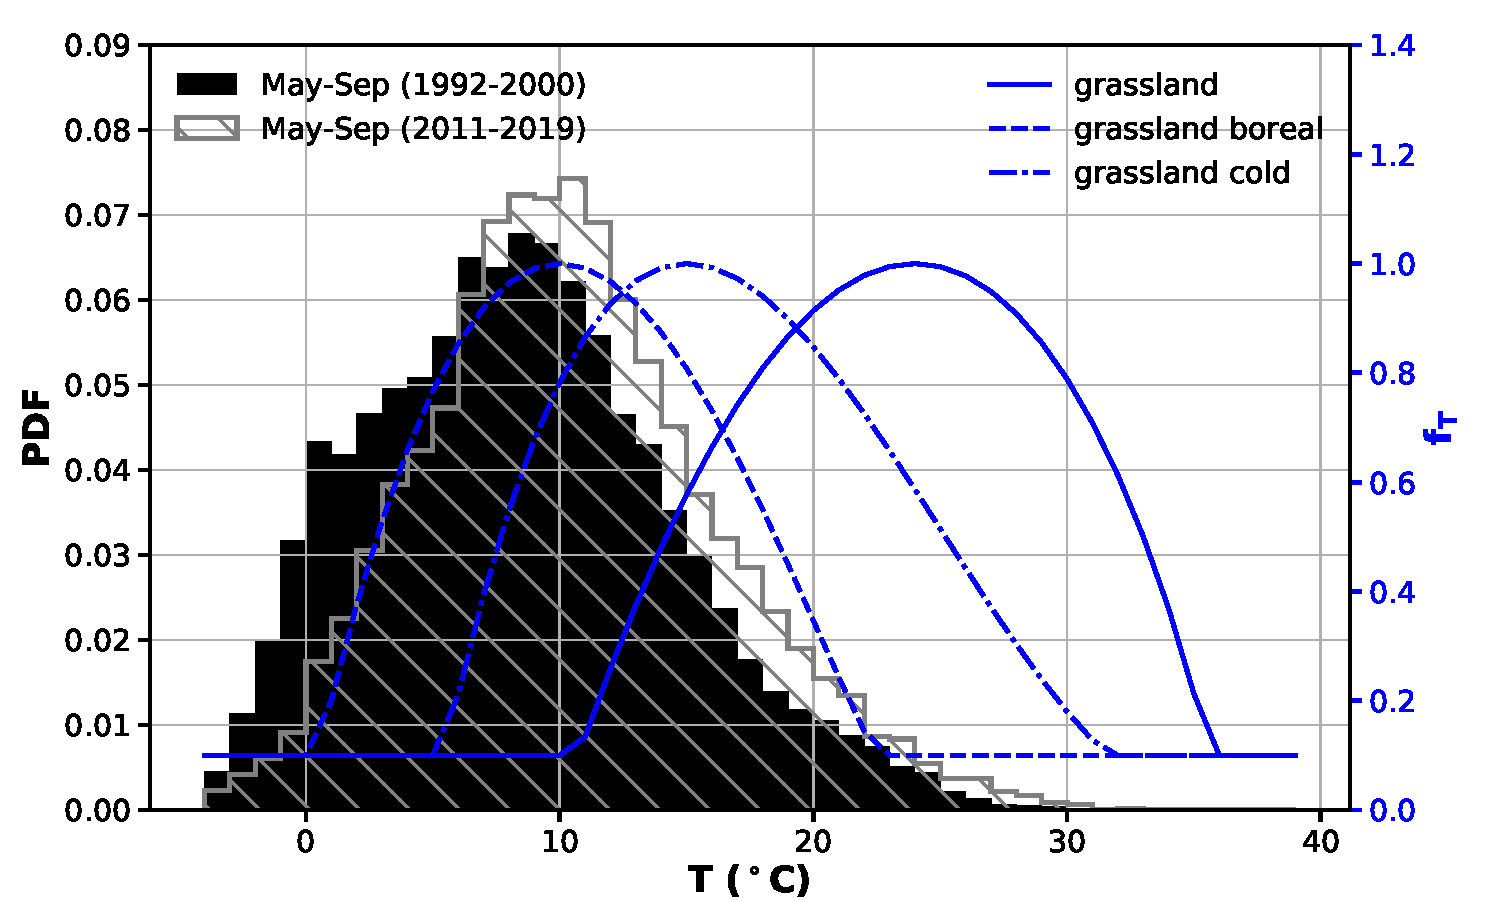
\includegraphics[width=8.3cm]{javis_funcs_temp_hist_grassland}\\
  %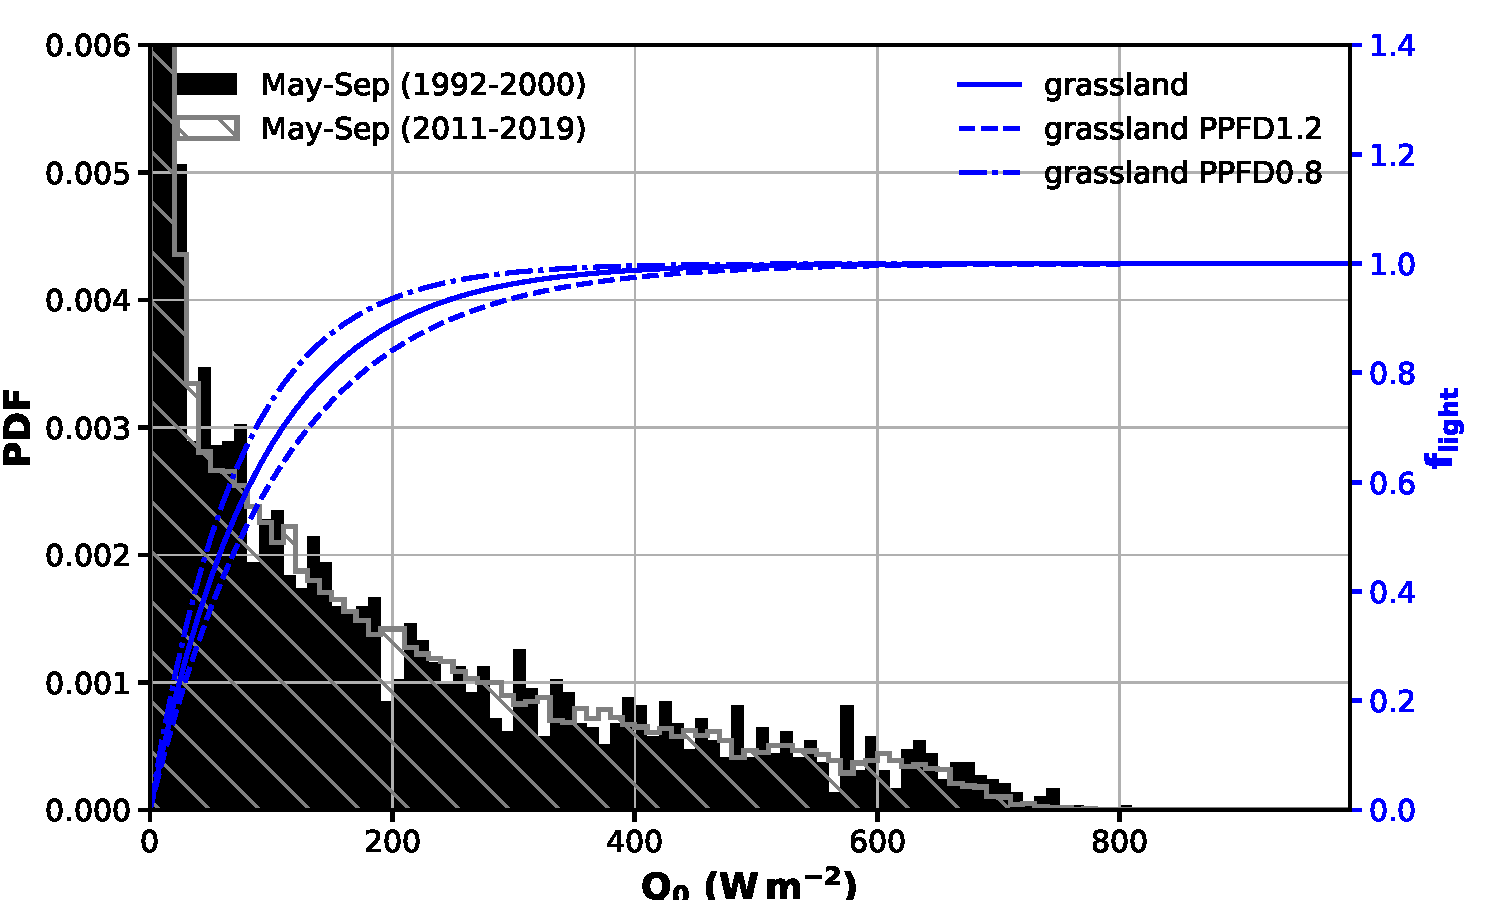
\includegraphics[width=8.3cm]{javis_funcs_rad_hist_grassland}
  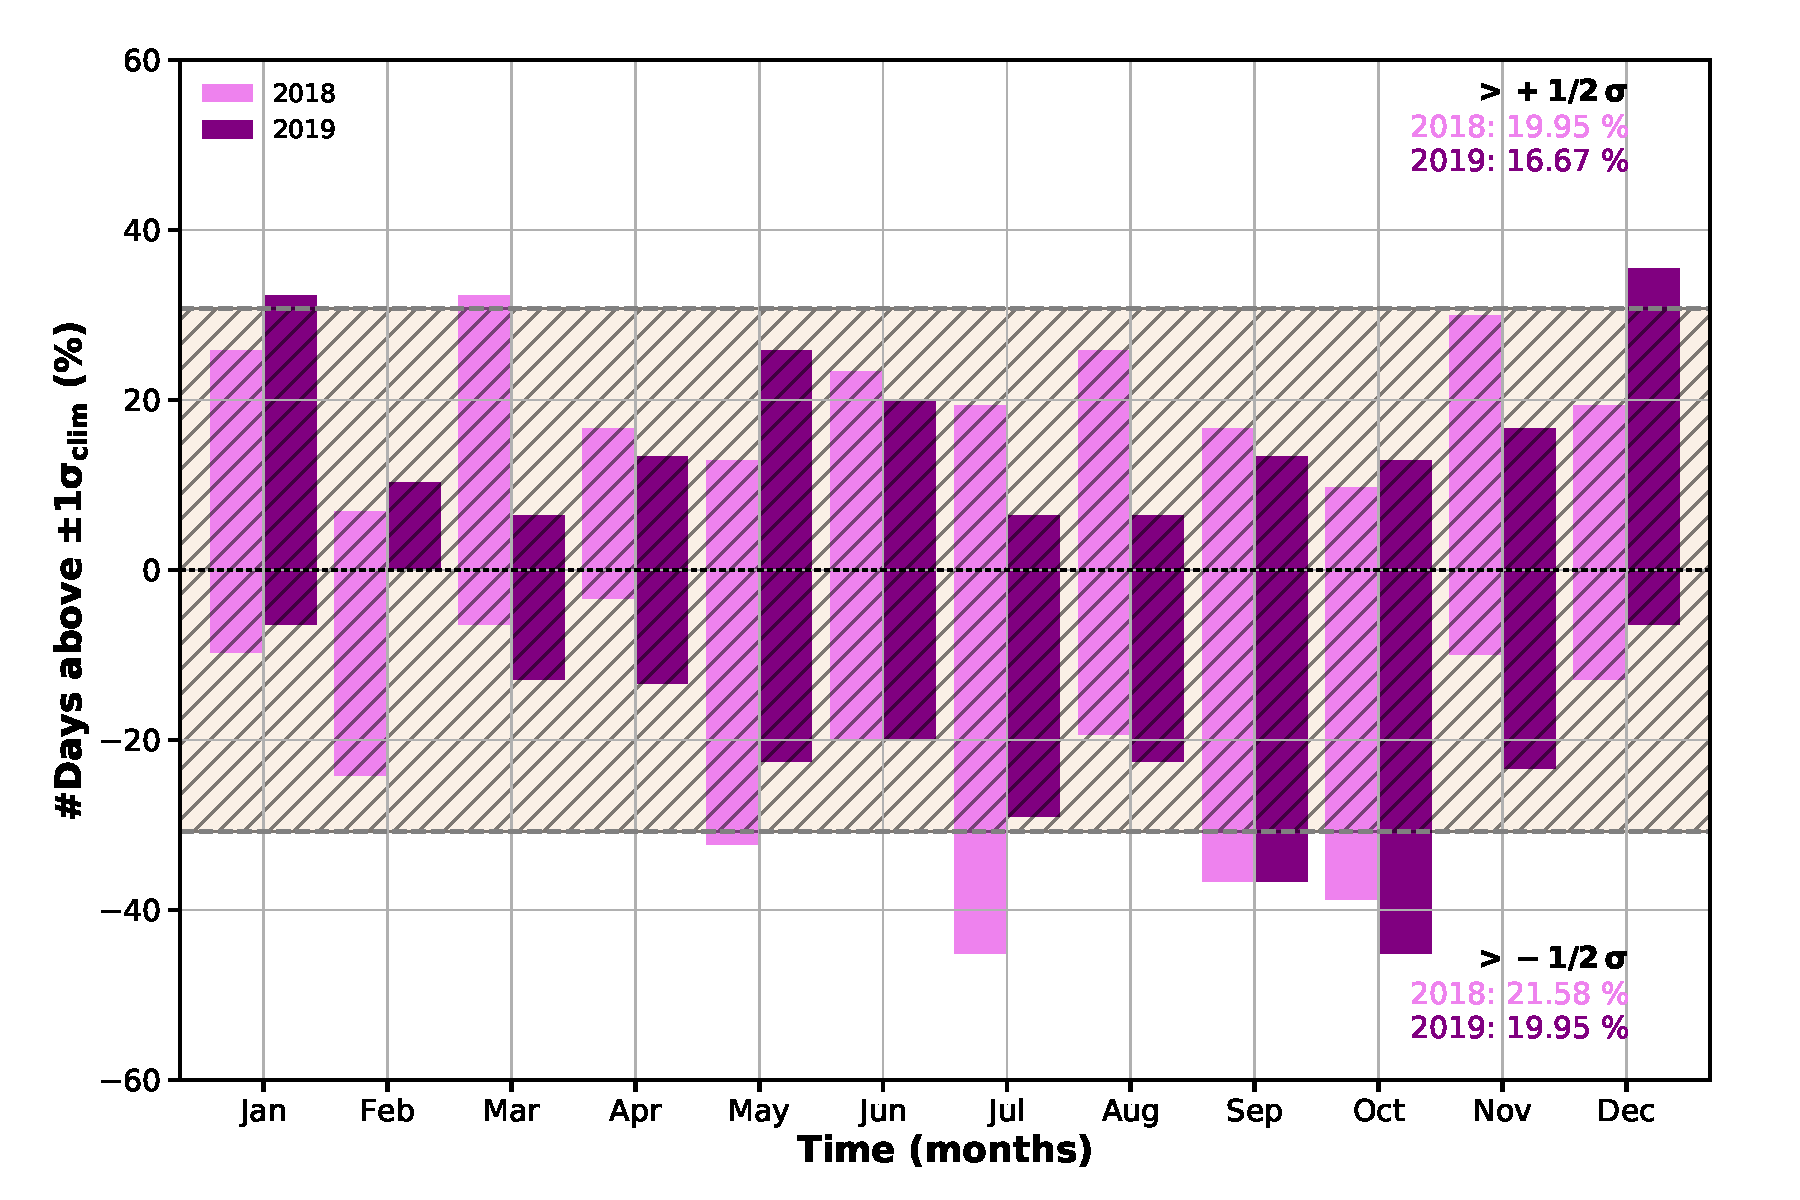
\includegraphics[width=8.3cm]{fig09}
\caption{Construction of bespoke response functions for grassland. (a) $f_\mathrm{T}$ and (b) $f_\mathrm{flight}$ are shown together with underlying $T_\mathrm{air}$ and $Q_0$ climatologies (probability density function - PDF), respectively. Original mapping manual parameterization is shown in comparison as solid line. Note that $Q_0$ has been truncated to $0.006$. PPFD0.8 and PPFD1.2 refer to $\alpha$ values increasing/decreasing PPFD at $f_\mathrm{light}=0.5$ by $\pm 20\,\%$, respectively.}
\label{fig:f_temp_grassland}
\end{figure}

\begin{table}[t]
  \caption{Bespoke temperature parameterizations. MM refers to mapping manual \citep{GCB:Mills2011,ICP:MappingManual2017}.}
  \label{tab:sensitivity_tests_temp}
  \begin{tabular}{llrrr}
    \tophline
    Species & type & $T_\mathrm{min}$ & $T_\mathrm{opt}$ & $T_\mathrm{max}$ \\
    \middlehline
    \multirow{3}{*}{Downy birch} & MM & 5 & 20 & 100\\
    & Boreal & 0 & 10 & 100\\
    & Cold & 5 & 15 & 100\\
    \middlehline
    \multirow{3}{*}{Norway spruce} & MM & 0 & 20 & 100\\
    & Boreal & 0 & 10 & 100\\
    & Cold & 0 & 15 & 100\\
    \middlehline
    \multirow{3}{*}{Perennial grassland} & MM & 10 & 24 & 36\\
    & Boreal & 0 & 10 & 24 \\
    & Cold & 5 & 15 & 36\\
    \bottomhline
    \end{tabular}
\end{table}

\begin{table}[t]
  \caption{Bespoke light parameterizations. MM refers to mapping manual \citep{GCB:Mills2011,ICP:MappingManual2017}.}
  \label{tab:sensitivity_tests_light}
  \begin{tabular}{llr}
    \tophline
    Species & type & $\alpha$\\
    \middlehline
    \multirow{3}{*}{Downy birch} & MM & 0.004 \\
    & PPFD0.8 & 0.005\\
    & PPFD1.2 & 0.004\\
    \middlehline
    \multirow{3}{*}{Norway spruce} & MM & 0.006 \\
    & PPFD0.8 & 0.008  \\
    & PPFD1.2 & 0.005  \\
    \middlehline
    \multirow{3}{*}{Perennial grassland} & MM & 0.011\\
    & PPFD0.8 & 0.014 \\
    & PPFD1.2 & 0.009 \\
    \bottomhline
    \end{tabular}
\end{table}

As indicated above, a better acclimation will result in a higher average $\left<g_\mathrm{sto}\right>/g_\mathrm{max}$. To quantify the resulting bespoke parameterizations, we propose the following metric. For a generic GS (May--August), we compute climatological average and standard deviation of $\left<g_\mathrm{sto}\right>/g_\mathrm{max}$ (Eq.~(\ref{eq:stomatal})) at noon (averaged over $11\,\unit{am}-1\,\unit{pm}$ local time) and in the morning (averaged over $5-9\,\unit{am}$ local time). We presume that relative stomatal conductance of around noon (highest light intensity) and in the early morning (lower intensities) are good proxies for \chem{CO_2} uptake efficiency. Our arbitrary optimization target is $60\,\unit{\%}$. Additional constrains are a small deviation between noon and morning and a low standard deviation indicating a higher robustness to interannual variability of growing conditions. For simplicity, we neglect the dependency on SWP in this regard. From the results shown in Fig.~\ref{fig:javis_func_opt_mean}, we identify boreal, PPFD0.8 as the best acclimation for all hypothetical species or PFTs alike. Overall, Norway spruce displays the least deviation between the different types of parameterizations, while the divergence for perennial grassland is substantial.  

\begin{figure}[t]
  %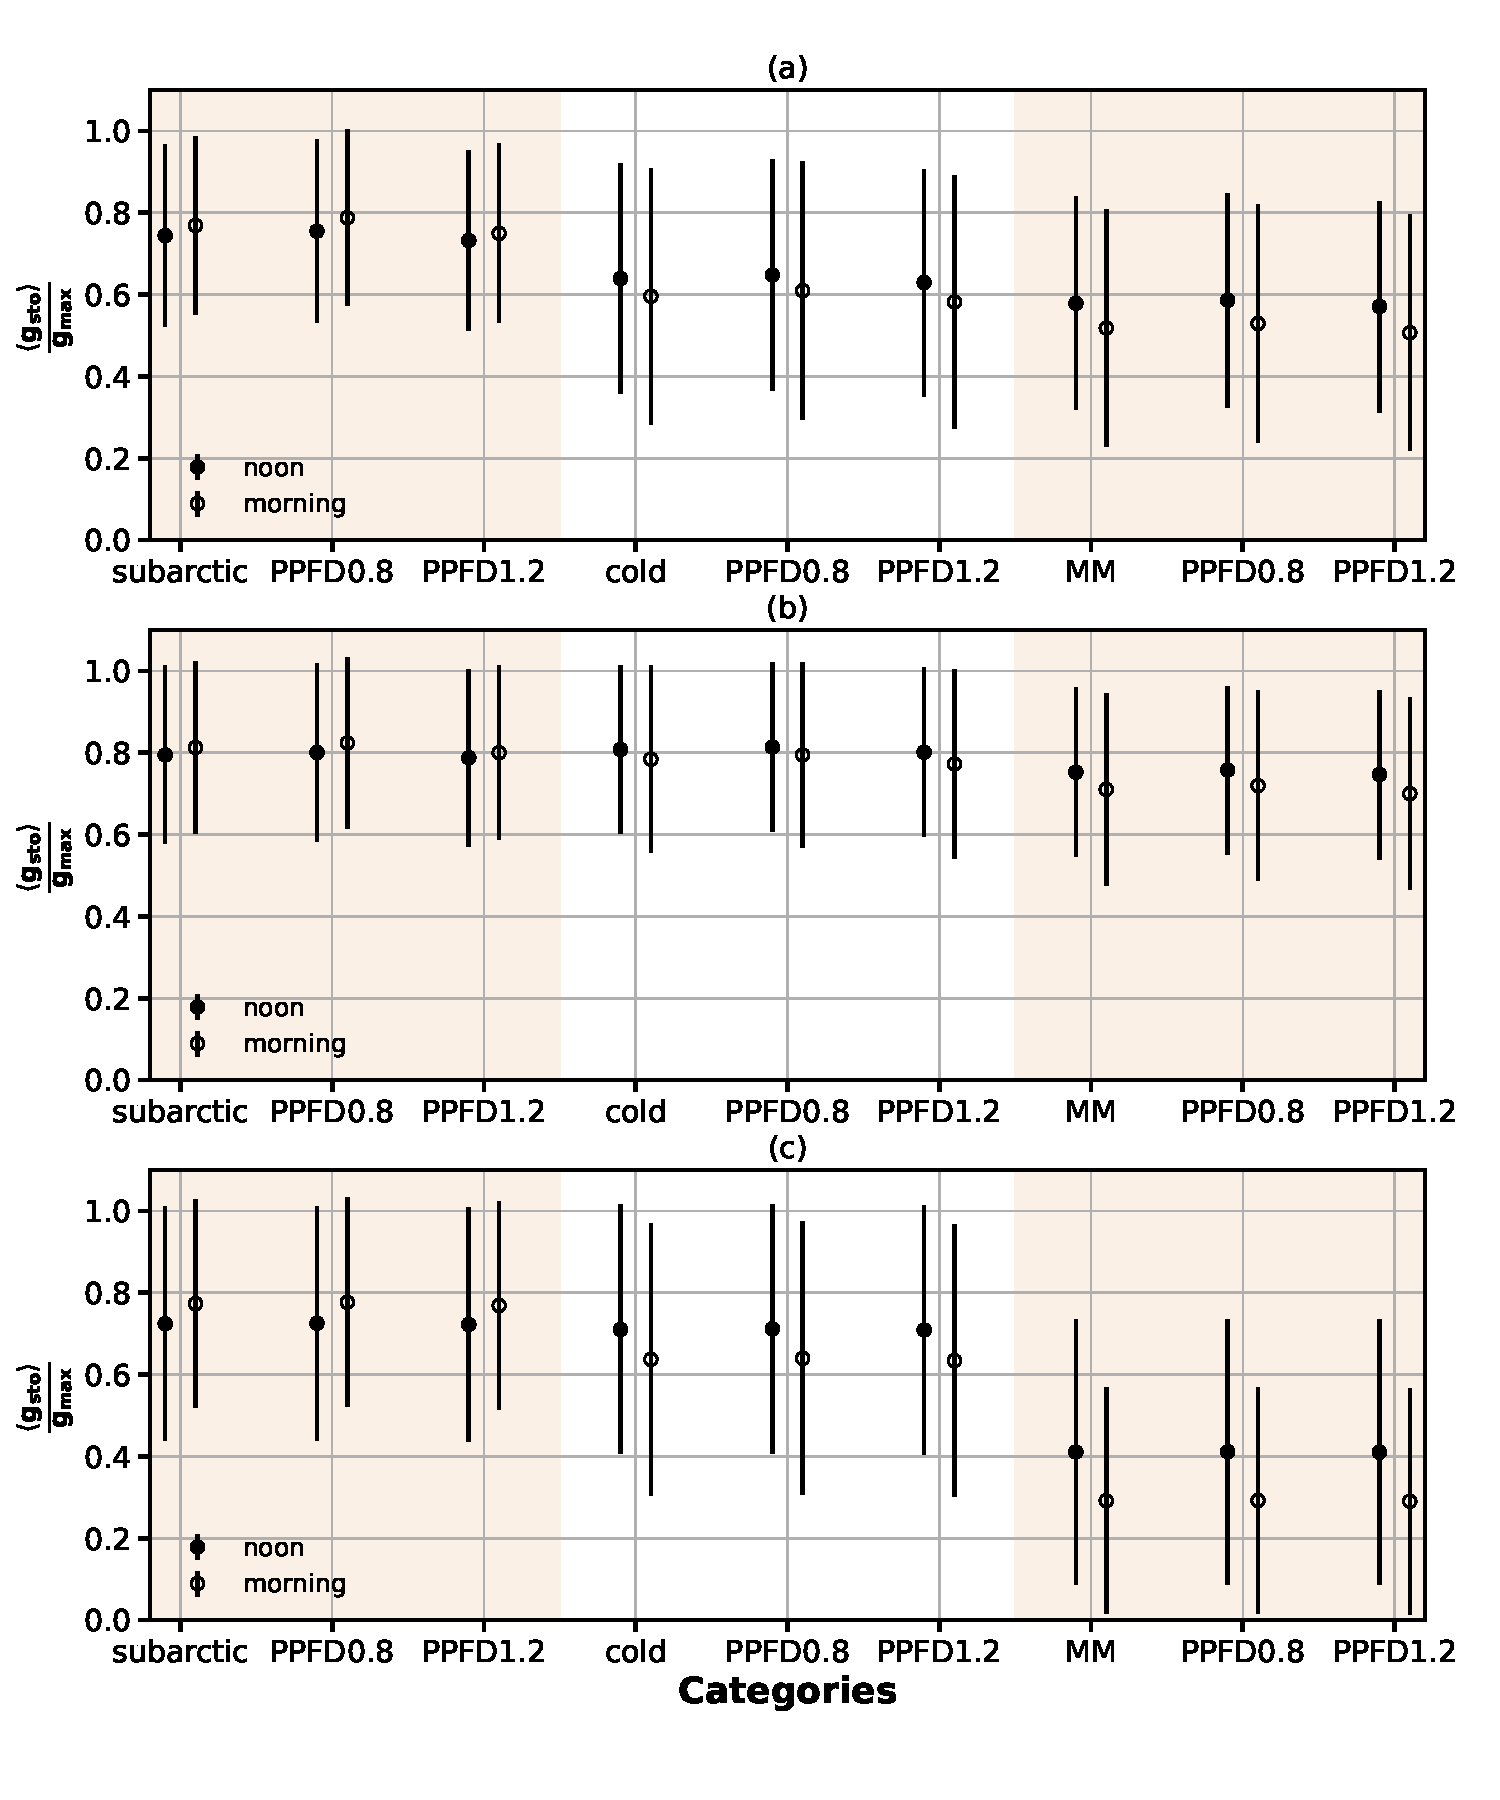
\includegraphics[width=8.3cm]{javis_func_opt_mean}
  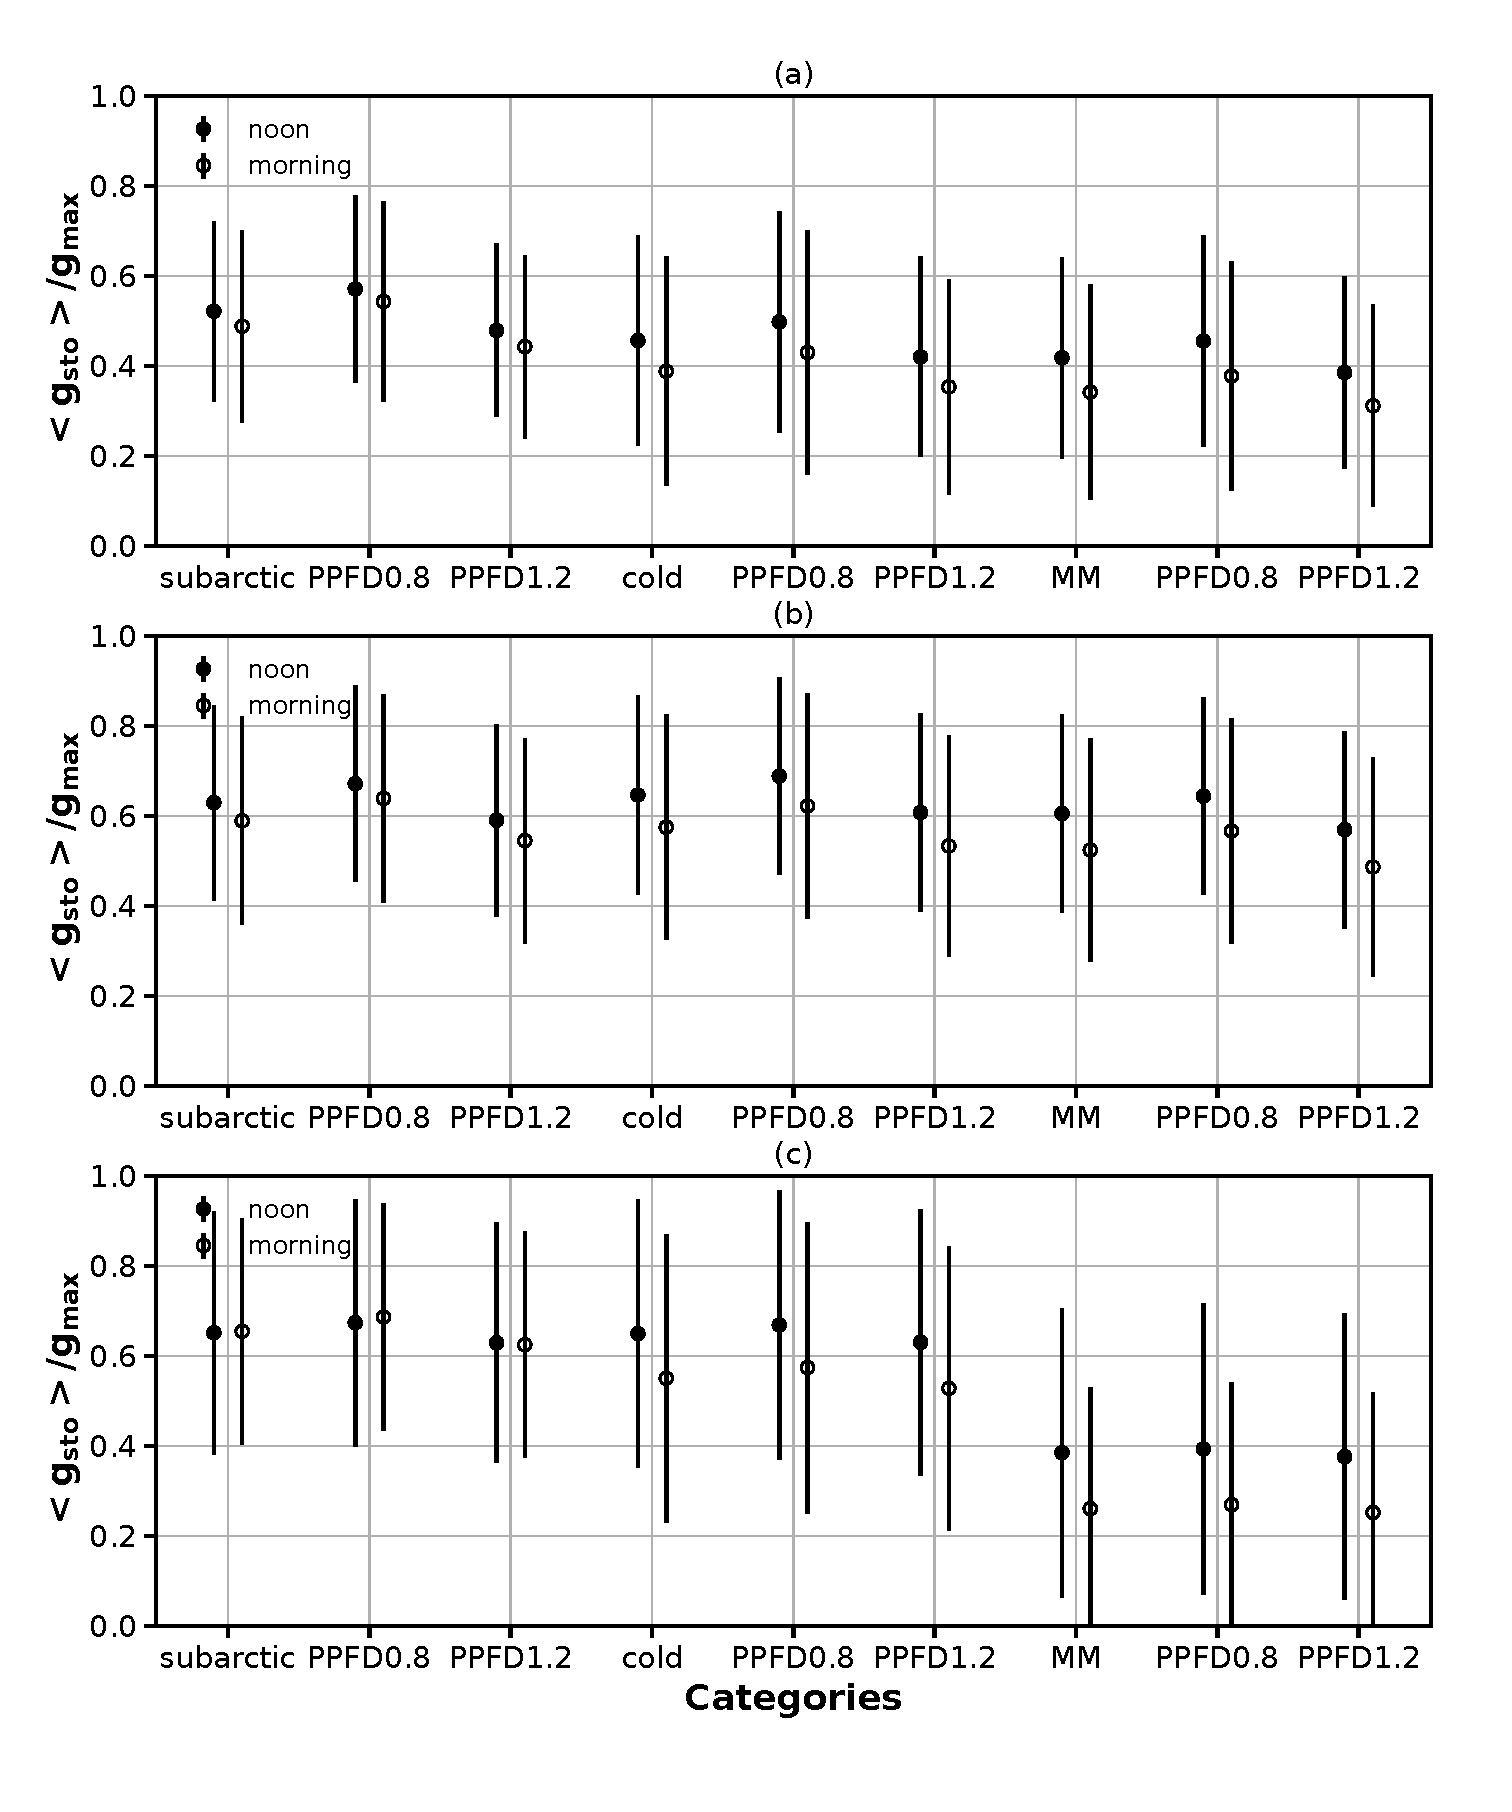
\includegraphics[width=8.3cm]{fig10}
  \caption{Proposed metric to test bespoke response functions. GS (May--August) climatological averages and standard deviation of $g_\mathrm{sto}^k$ (Eq.~(\ref{eq:stomatal})) relative to $g_\mathrm{max}^k$ at noon (averaged over $11\,\unit{am}-1\,\unit{pm}$ local time) and in the morning (averaged over $5-9\,\unit{am}$ local time) are shown for (a) Downy birch; (b) Norway spruce; (c) perennial grassland. For simplicity, $f_\mathrm{SWP}$ is neglected in this calculation. }
  \label{fig:javis_func_opt_mean}
\end{figure}

Another important factor for ozone exposure metrics is the timing and length of the GS. Start ($A_\text{start}$) and end ($A_\text{end}$) of GS for each PFT are given in units of \unit{doy} (Tab.~\ref{tab:sensitivity_tests_gs}) and estimated as follows. Evergreen needle leaf trees show photosynthetic activity already at low temperatures \citep{TP:Wallin2013, TB:Kolari2007}. We use a MODIS (Aqua/Terra) retrieved net photosynthesis product for a $1\times 1\,\unit{km}$ patch centered at Svanhovd to determine $A_\text{start}$ and $A_\text{end}$. Net photosynthesis data can be approximated by a second order polynomial function (Fig.~\ref{fig:modis_Psn}). By calculating the roots of the fitted polynomial, we derive $A_\text{start} = 122\,\unit{doy}$ for 2018 and \unit{doy} 106 in 2019. $A_\text{end}$ amounts to \unit{doy} 261 and 274, respectively, and is the value used for all PFTs. The resulting growing season for Norway spruce in 2019 was one month longer then in 2018. For estimating $A_\text{start}$ of downy birch, we use the $5$ consecutive days above $5\,\unit{^\circ C}$ agricultural rule of thumb on gridded temperature data from SeNorge.no (Fig.~\ref{fig:greening_season_change_Svanvik}). We find 129 and 130, respectively. For both years, these dates coincident with the first snow-free day at the meteorological weather station at Øvre Neiden (Sør-Varanger, NOR) which is relatively close-by.
For comparison, we would get $A_\mathrm{start} = 100\,\unit{doy}$ and $A_\mathrm{end} = 307\,\unit{doy}$ from the latitude model typically used for localizing $\mathrm{DO_3SE}$. By comparison, the latitude model indicates about a $2\,\unit{month}$ longer growing season. Due to a lack of quantitative field observation, we assume a latency period of about $1\,\unit{month}$ after snow-melt for perennial grassland. 

\begin{table}[t]
  \caption{Bespoke start and end of growing season in units of \unit{doy}. MM refers to mapping manual \citep{GCB:Mills2011,ICP:MappingManual2017}.}
  \label{tab:sensitivity_tests_gs}
  \begin{tabular}{llcc}
    \tophline
    Species & Year & $A_\mathrm{start}$ & $A_\mathrm{end}$\\
    \middlehline
    \multirow{2}{*}{Downy birch} & 2018 & 129$^*$ & 261$^\dagger$ \\
    & 2019 & 130$^*$ & 274$^\dagger$ \\
    \multirow{2}{*}{Norway spruce} & 2018 & 122$^\dagger$ & 261$^\dagger$ \\
    & 2019 & 106$^\dagger$ & 274$^\dagger$ \\
    \multirow{2}{*}{Perennial grassland} & 2018 & 159$^\ddagger$ & 261$^\dagger$\\
    & 2019 & 161$^\ddagger$ & 274$^\dagger$ \\
    \bottomhline
  \end{tabular}
  \belowtable{$^\dagger$ MODIS (Aqua/Terra) net photosynthesis product;\\
    $^*$ $5\,\unit{days}-5\,\unit{^\circ C}$-rule, $T_\mathrm{air}$ from \href{seNorge.no}{seNorge.no};\\
    $^\ddagger$ One month after snow melt; reference station Øvre Neiden (Sør-Varanger, NOR)} % Table Footnotes
\end{table}


As pointed out by \citet{ACP:Bueker2012}, a very important factor in deriving a proper $\mathrm{POD_y}$ is the soil texture or how much water the soil can hold. As Svanhovd is located in the bed of the Pasvik river, we assume a sandy loam texture at $60\,\unit{cm}$ depth. The estimate of leaf boundary layer resistance is a function of wind speed which will be influenced by the tree height and leaf dimensions. Leaves of downy birch in northern Fennoscandia are smaller than southern specimens' with leaf dimensions of $(3.0\pm 0.5)\,\unit{cm}$. In addition, \citet[][p.~52]{NINA2004} indicate an average tree height of $13.5\,\unit{m}$ in the area. Both these factors will affect leaf boundary layer resistance, the smaller leaves would tend to reduce leaf boundary layer resistances whilst the shorter trees would reduce canopy roughness and increase canopy boundary layer resistances.

\subsection{$\mathrm{POD_1}$ results and implications on ozone impact}
\label{subsec:do3se_results}

We have modeled $\mathrm{POD_y}$ with a flux threshold $y=1\,\unit{nmol\,m^{-2}\,s^{-1}}$ per projected leaf area (PLA) for three natural/semi-natural vegetation types, downy birch, Norway spruce, and perennial grassland using both MM parameterizations and a variety of bespoke response function in $f_\mathrm{T}$ and $f_\mathrm{light}$, and localized GS (described in detail in Section~\ref{subsec:do3se_parameters}). The results are shown in Fig.~\ref{fig:pody_rel}. For comparison, critical levels for a $4\,\unit{\%}$ (silver birch), $2\,\unit{\%}$ (Norway spruce) \citep{ICP:MappingManual2017}, and $10\,\unit{\%}$ (perennial grassland, above ground) \citep{ESPR:Hayes2021} reduction in biomass are shown as horizontal dashed lines. Different years are color coded as previously. Simulations with MM GS, canopy, and leaf parameters are indicated with squared markers, bespoke GS with circles. The annotation $\pm$ refers to bespoke light response function threshold ($+\rightarrow\mathrm{PPFD1.2}$, $-\rightarrow\mathrm{PPFD0.8}$), while bespoke temperature response functions are indicated by categories on the x-axis. Closed/open symbols represent SWP sensitivity switched off/on in the model.

The results depicted in Fig.~\ref{fig:pody_rel} allow for a comprehensive assessment of a large variety of systematic uncertainties in the exposure-based risk metric for ozone induced damage in subarctic vegetation. In summary, we identify the following main effects of the bespoke parameterizations of the $DO_3SE$ model with respect to the MM default parameterization on ozone uptake:
\begin{itemize}
  \itemsep0pt
\item Increasing cold tolerance/heat intolerance $\Rightarrow$ increased uptake in both probed years,
\item usage of proper growing season $\Rightarrow$ reduced uptake with respect to the increase reported above,
\item an earlier assumed start of GS $\Rightarrow$ increased uptake,
\item drought conditions (SWP) $\Rightarrow$ reduced uptake,
\item lower/higher extent of stomatal opening at low light intensities $\Rightarrow$ increased/reduced uptake,
\item symmetric variation of the extent of stomatal opening at low light intensities $\Rightarrow$ asymmetric response in POD,
\item temperature acclimation $\Rightarrow$ amplifying effect on light threshold and drought effects.
\end{itemize}
The exact order of magnitude of these effects varies for individual species or PFTs and between years, but the predicted ozone uptake for the bespoke parameterization is always larger than for the MM default parameterizations and of the same order of magnitude as the variability between the years studied here. Although our temperature acclimations are hypothetical, they suggest considerable underestimations of ozone risk for subarctic species when compared to generic MM parameterizations. In particular, an earlier GS due to climate change, that is overlapping with the ozone spring peak, has the potential to increase the risk of ozone damage for vegetation with an acclimation to cold climates. Drought effects (SWP) do only matter if a bespoke GS is not taken into account. We will look at the specific species or PFTs in more detail in the following.

For downy birch (Fig.~\ref{fig:pody_rel}a) all simulations exceed the CL by $5-25\,\unit{mmol\,\chem{O_3}\,m^{-2}}$. Downy birch displays the largest variance of ozone uptake among all species or PFTs ($10-31\,\unit{mmol\,\chem{O_3}\,m^{-2}}$). In particular, the sensitivity to the light threshold is especially pronounced, e.g. $\Delta\mathrm{POD_1} = ^{+2.5}_{-3.6}\,\unit{mmol\,\chem{O_3}\,m^{-2}}$ in case of the boreal type without bespoke GS in 2019. Without bespoke GS, 2018 displays a higher ozone damage risk than 2019. However, taking the later start and overall shorter GS in 2018 into account, this is reversed for the boreal acclimation type. This can be partly explained by very high light response factors (over $f_\mathrm{light}>0.8$) in the beginning of the GS in these simulations. Whether this is a bug or a feature of the $\mathrm{DO_3SE}$ model is not clear. SWP induced reduction in ozone uptake is only effective in 2018 and without bespoke GS. The temperature acclimation dependent bias in ozone uptake deduced for bespoke GS ranges between $(1.4-3.6)\,\unit{mmol\,\chem{O_3}\,m^{-2}}$ in 2018 and $(2.7-7.7)\,\unit{mmol\,\chem{O_3}\,m^{-2}}$ in 2019. The maximum systematic deviations deduced from the $-20\,\unit{\%}$ (superscript) and $+20\,\unit{\%}$ (subscript) variation of the extent of stomatal opening at low light intensities amount to $^{+1.6}_{-2.3}\,\unit{mmol\,\chem{O_3}\,m^{-2}}$ and $^{+1.9}_{-2.7}\,\unit{mmol\,\chem{O_3}\,m^{-2}}$, respectively. 

For Norway spruce (Fig.~\ref{fig:pody_rel}b), most simulations slightly exceed the CL ($0-10\,\unit{mmol\,\chem{O_3}\,m^{-2}}$). Norway spruce is the least sensitive to an acclimation in temperature and therefore the least biased compared to the generic default MM parameterization. Norway spruce displays a medium sensitivity to the variation in the light threshold, e.g. $\Delta\mathrm{POD_1} = ^{+1.7}_{-1.3}\,\unit{mmol\,\chem{O_3}\,m^{-2}}$ in case of boreal type without bespoke GS in 2018. Taking the bespoke GS into account, we find a higher ozone uptake in 2019 for all bespoke temperature response functions. The overall bias deduced from bespoke GS for boreal and cold types with respect to MM ranges between $(0.5-1.0)\,\unit{mmol\,\chem{O_3}\,m^{-2}}$ in 2018 and $(2.0-3.3)\,\unit{mmol\,\chem{O_3}\,m^{-2}}$ in 2019. The maximum systematic deviations deduced from the $-20\,\unit{\%}$ (superscript) and $+20\,\unit{\%}$ (subscript) variation of the extent of stomatal opening at low light intensities amount to $^{+1.0}_{-0.8}\,\unit{mmol\,\chem{O_3}\,m^{-2}}$ and $^{+1.3}_{-1.0}\,\unit{mmol\,\chem{O_3}\,m^{-2}}$, respectively.

For perennial grassland (Fig.~\ref{fig:pody_rel}c), all simulations with bespoke GS stay below the CL. Perennial grassland shows the smallest ozone uptake, but a similarly large bias as downy birch. We also find a reversal for predicted ozone damage risk in $\mathrm{POD_1}$ between 2018 and 2019 for the boreal type. Perennial grassland shows the lowest sensitivity to the light threshold and SWP is only relevant without bespoke GS. The overall bias deduced from bespoke GS for boreal and cold types with respect to MM ranges between $(2.2-3.4)\,\unit{mmol\,\chem{O_3}\,m^{-2}}$ in 2018 and $(4.4-6.4)\,\unit{mmol\,\chem{O_3}\,m^{-2}}$ in 2019. The maximum systematic deviations deduced from the $-20\,\unit{\%}$ (superscript) and $+20\,\unit{\%}$ (subscript) variation of the extent of stomatal opening at low light intensities amount to $^{+0.3}_{-0.2}\,\unit{mmol\,\chem{O_3}\,m^{-2}}$ and $^{+0.3}_{-0.3}\,\unit{mmol\,\chem{O_3}\,m^{-2}}$, respectively.

\begin{figure}[t]
  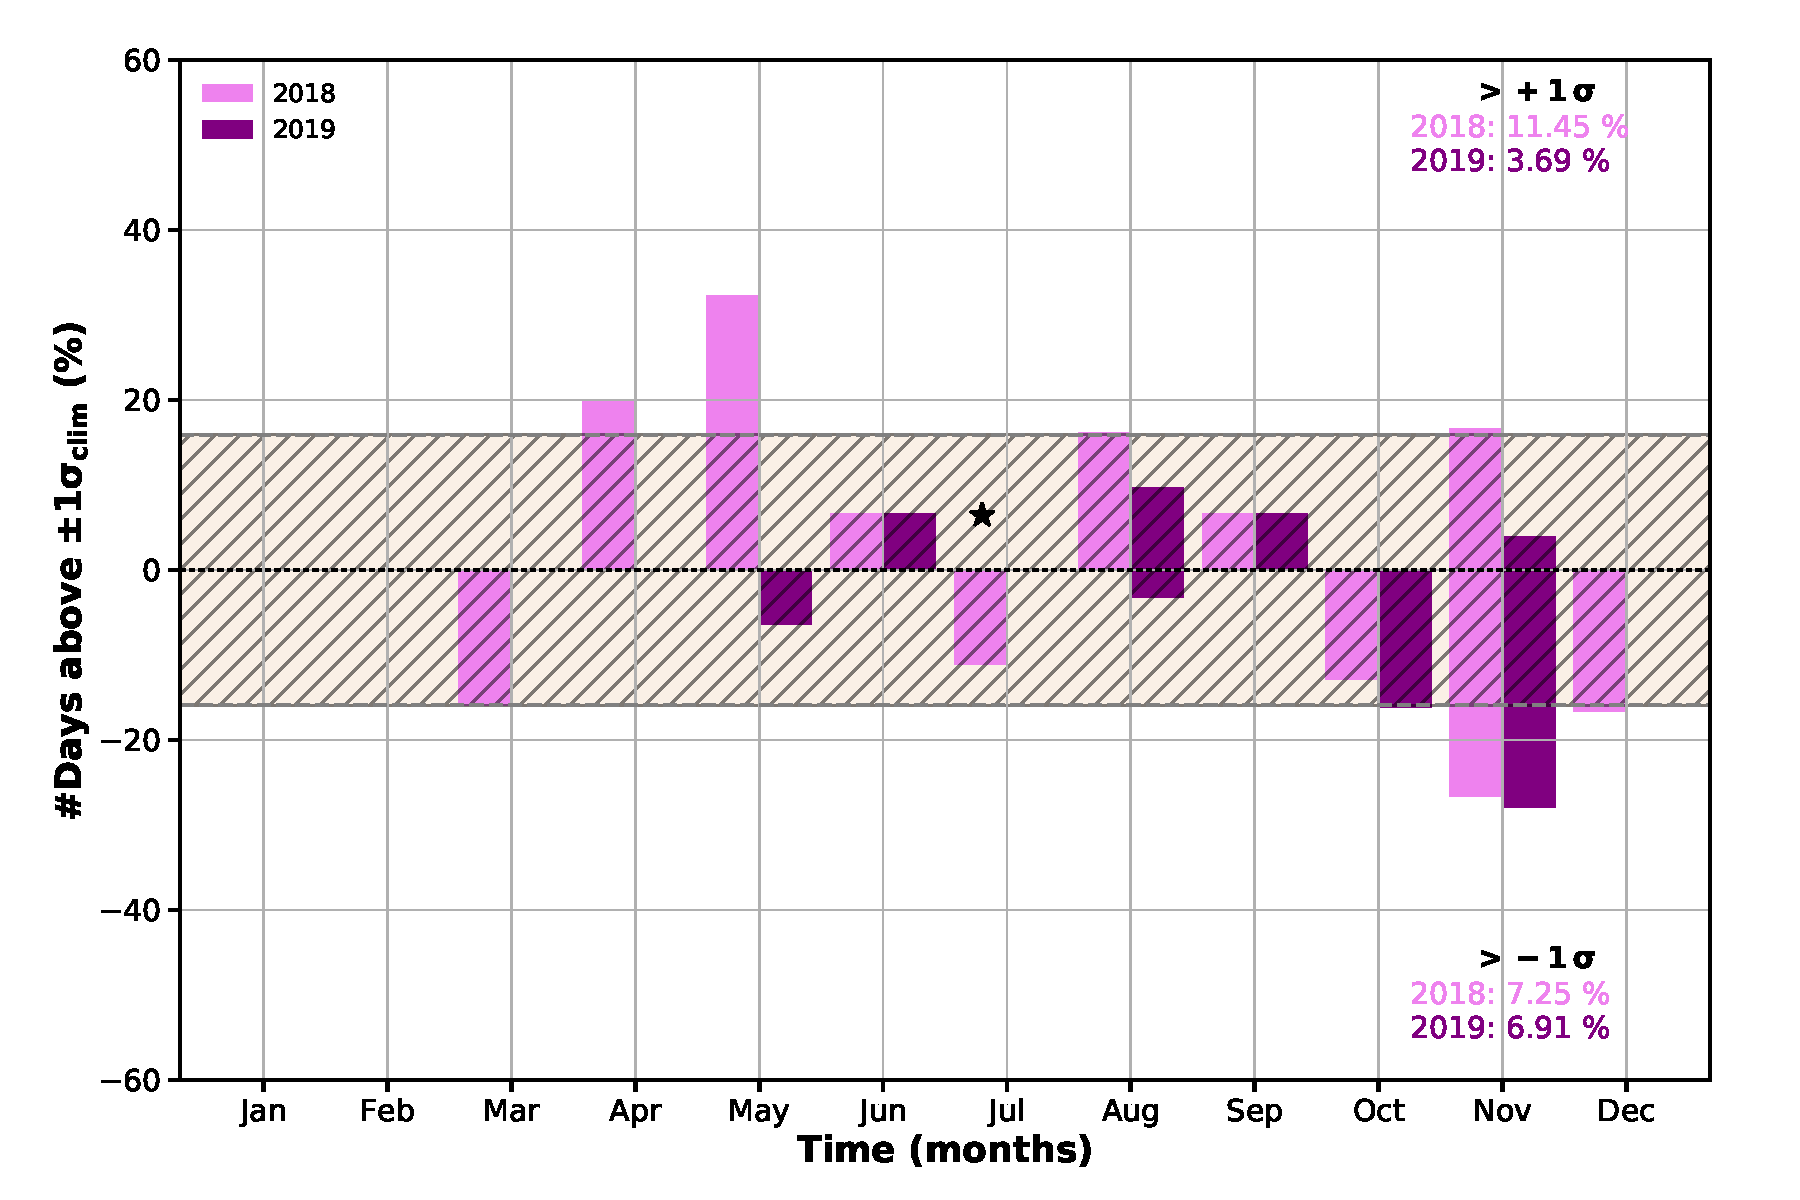
\includegraphics[width=8.3cm]{fig11}
  \caption{$\mathrm{DO_3SE}$ modeling results for $\mathrm{POD_1}$ with default parameterization (MM) and bespoke parameters for Svanhovd. Bespoke parameterizations include temperature response functions for boreal, cold and light thresholds (PPFD0.8, PPFD1.2) at the end of a MM GS (lighter hue and dotted lines) and the estimated GS for Svanhovd (2018, 2019). (a) Downy birch; (b) Norway spruce; (c) Perennial grassland. The dashed horizontal lines indicate critical levels defined in \citet{ICP:MappingManual2017,ESPR:Hayes2021} for each species, respectively.}
  \label{fig:pody_rel}
\end{figure}

We estimated the biomass reductions in accordance to the CLs in \citet{ICP:MappingManual2017, ESPR:Hayes2021} for the most extreme temperature acclimation (\emph{boreal}) for each bespoke PFT. The estimates are listed in Table~\ref{tab:biomass_reduction}. The reported range in uncertainty corresponds to the maximum deviation defined by the $\pm 20\,\unit{\%}$ variation of the extent of stomatal opening at low light intensities with SWP=on. For downy birch and perennial grassland, substantial reductions in total biomass in comparison with the default generic MM parameterizations are predicted for both years. Norway spruce is the least affected and the magnitude of total biomass reduction is independent of the choice of the parameterization within given uncertainties. This may reflect the more comprehensive research on this species or PFT. The systematic deviation for downy birch is one order of magnitude larger than for Norway spruce and perennial grassland.

From the difference between 2018 and 2019, we infer a substantial interannual variability. The interannual variability is estimated to be larger than our reported systematic deviations and can be of the same order of magnitude as the effect of the temperature acclimation. This means that the choice of temperature acclimation has the potential to either revoke or amplify the risk of ozone damage for vegetation. However, the risk of ozone damage in downy birch and perennial grassland in comparison with the generic default MM parameterizations is increased, regardless.

\begin{table}[t]
  \caption{Estimated total biomass reduction in \unit{\%} for temperature acclimation \emph{boreal} with bespoke GS and SWP=off. The uncertainty ranges reported here correspond to maximum a divergence deducted from varying the extent of stomatal opening at low light intensities and SWP=on. For comparison, the corresponding biomass reduction for the generic default MM averaged over both years is shown. The reported standard deviation is computed from all sensitivity simulations ($\pm 20\,\unit{\%}$ in extent of stomatal opening at low light, SWP on/off, and bespoke GS).}
  \label{tab:biomass_reduction}
\begin{tabular}{lllll}
\tophline
Year & \multicolumn{4}{c}{PFT}\\
& Downy birch & Norway spruce & \multicolumn{2}{c}{Perennial grassland}\\
\middlehline
2018 & $15.5^{+(1.9...2.1)}_{-(0.8...1.5)}$ & $2.5^{+0.2}_{-0.2}$ & $9.7^{+0.2}_{-0.2}$ & $^*12.4^{+0.2}_{-0.2}$\\
2019 & $17.4^{+2.5}_{-1.8}$ & $3.0^{+0.2}_{-0.3}$ & $10.5^{+(0.1...0.2)}_{-(0.0...0.1)}$ & $^*13.7^{+(0.1...0.3)}_{-(0.1...0.3)}$\\
\middlehline
$\left<\mathrm{MM}\right>$ & $11.2\pm 1.1$ & $2.31\pm 0.04$ & $7.5\pm 0.9$ & $^*9.6\pm 1.4$\\
\bottomhline
\end{tabular}
\belowtable{$^*$ above ground biomass} % Table Footnotes
\end{table}


\conclusions[Discussion and conclusions]
\label{sec:conc}

We have studied the effect of acclimations of biomes to a subarctic climate on phyto-toxic ozone uptake. The comparison between 2018 and 2019 conditions allowed us to consider these acclimations and their influence on vegetation sensitivity to \chem{O_3} in light of future changes of key environmental variables as may occur under climate change (e.g. increase of frequency and extent of heatwaves). We found that conditions for ozone formation were more favorable in the 2018 growing season than in 2019, with 2018 being significantly warmer and less cloudy in spring and early summer. Accordingly, peak ozone concentrations occurred more frequently and at higher levels in 2018. This was particularly a result of the extended heatwave in spring and early summer and associated, extensive wildfires in Central Sweden (in particular in mid--end July).

We found that the length and timing of the growing season are crucial for risk assessment based on accumulated ozone flux metrics ($\mathrm{POD_y}$). Based on a MODIS photosynthesis product, we estimated the growing season for Norway spruce in 2018 to be at least one month shorter than in 2019. The found start of growing season in 2018 ($122\,\unit{doy}$) and 2019 ($106\,\unit{doy}$) are within given ranges by empirical observations \citep{TB:Kolari2007,IVL:Karlsson2018}. Based on gridded observational temperature and snow depth, we found a half a month shorter growing season for downy birch and perennial grassland in 2018 compared to 2019, respectively. The timing and emerging trend in the start of the growing season may differ substantially between local observation and common thermal or latitudinal estimations. Species-specific methods show a later start for European silver birch and an earlier for Norway spruce, compared to the thermal growing season \citep{IVL:Karlsson2018}. With respect to ongoing climate change, a clear positive trend in length ($5.2\,\unit{d\,decade^{-1}}$) almost equally distributed between earlier start ($2.9\,\unit{days\,decade^{-1}}$) and later end ($2.3\,\unit{d\,decade^{-1}}$) could be deducted from the thermal growing season at Svanhovd.

We found representative ozone climatologies (multi-annual means) for northern Fennoscandia and Svanhovd based on ground-level ozone monitoring. To account for missing data from our 2018 record, we proposed a routine for gap filling of ozone observations following a Reynolds's decomposition into anomalies and climatology. In the course, we also assessed the quality of available global (MACC and CAMS) and regional (CAMS Regional Air Quality (CAMSRAQ) ensemble) reanalysis products for Europe concerning ozone. We have studied the ozone seasonality for northern Fennoscandia and the quality of its representation in available global and regional reanalysis products for Europe. We confirm that both global reanalysis products do not reproduce the observed ozone patterns in northern Fennoscandia \citep{GMD:Huijnen2020,ACPD:Barten2020}. Only the CAMSRAQ ensemble reproduces the observed ozone seasonality, although with a remaining low-bias. This confirms that high spatial resolution and assimilation of in situ observations of ground-level ozone concentrations are a must to constrain reanalysis products related to air quality and risk assessment ozone damage to vegetation, especially in high latitudes.

Ozone peak concentrations were observed more frequently in 2018 than in 2019. In 2018, we found significantly enhanced \chem{[O_3]} particularly in April and May, but not during the active wildfires in July. This suggests that weather conditions and high ozone concentration at the beginning of the growing season are more important in risk assessment using flux-based metrics than episodes of peak concentrations over shorter periods. Because these peak \chem{[O_3]} may coincident with environmental conditions that limit ozone uptake and hence do not lead to damage. Consequently, acute cellular damage caused by very high fluxes over a short period is not accounted for properly in $\mathrm{POD_y}$. As pointed out by \citet{AE:Musselman2006}, a higher temporal resolution, e.g. susceptibility to ozone depending on leaf age, in the associated damage functions might give a different picture. For herbal and grassland species (similar for crops) a strong dependency on the phenological state, e.g. high susceptibility to ozone in the reproductive state, was found \citep{EP:Bassin2004}. 

To estimate potential biases in the assessment of ozone-induced risk on Fennoscandia vegetation, we defined hypothetical temperature response functions representing different levels of assumed acclimation to cold climates. We assume northern Fennoscandia vegetation to be more tolerant towards cold temperatures and less tolerant to heat. Based on probability density functions (PDF) of observed light and temperature, we assume that an acclimation ought to increase the enclosed area between the respective response functions and the PDF. These hypothetical species or PFTs still need verification by experimental data.

In summary, our key findings are:
\begin{enumerate}
   \itemsep0pt
 \item the bespoke parameterizations for subarctic species are important (especially concerning light and temperature and the climate effect on the growing season) to be able to assess \chem{O_3} uptake,
 \item the parameterizations defined in the mapping manual for European regional risk assessment would appear to not adequately capture the physiological responses of subarctic physiology that are important determinants of \chem{[O_3]} sensitivity under prevailing environmental conditions and are likely to substantially underestimate risk,
 \item the ozone reanalysis products tend to underestimate \chem{[O_3]} in Fennoscandia, and
 \item that the climatic conditions promoting ozone damage (particularly extended heatwaves and the timing of the growing season concerning the ozone spring peak) and which are likely to become more frequent under climate change are likely to further enhance the sensitivity of subarctic vegetation to ozone.
\end{enumerate}

However, the decline of the ozone spring peak is partly caused by dry deposition of ozone on vegetation. It, therefore, remains unclear whether an earlier start of the growing season has the potential to reduce the ozone spring peak concentration compared to present-day and hence reduce the damage risk of ozone in the future. 
We have not assessed the effect of the plants' response to VPD here, but our climatological data show that conditions at Svanhovd are shifting towards a more VPD limited regime.
 
Based on the methods described in \citet{ICP:MappingManual2017}, we estimated biomass reductions due to ozone uptake for both 2018 and 2019 and find significant reductions for downy birch ($15.5-17.4\,\unit{\%}$) and perennial grassland (above ground, $12.4-13.7\,\unit{\%}$) with respect to estimates based on $\mathrm{POD_1}$ from default parameterizations. For Norway spruce, the results are compatible with the default parameterization estimates and are contained within the range of systematic uncertainties deduced from our bespoke response function ($2.5-3\,\unit{\%}$). These results have to be treated with care because the biomass reduction functions were not established based on subarctic species and might as well be subject to biases.  

At the same time, intra-species variability even at the same location is typically non-negligible \citep{EP:Bassin2004,Amb:Girgzdiene2009}. This may explain contradictory results regarding the ozone sensitivity of natural vegetation in northern Europe. While \citet{FS:Subramanian2014} reported a modeled reduction of net primary production in Norway spruce ($4.3-15.5\,\unit{\%}$) and birch ($1.4-4.3\,\unit{\%}$) under elevated ozone in Sweden, Lithuanian forest deciduous trees were observed to be more susceptible to visible damage by ozone than Norway spruce \citep{Amb:Girgzdiene2009}. Open-top chamber (OTC) experiments performed in northern Finland where Scots pine and downy birch were exposed to elevated ozone concentrations showed biomass reductions of both downy birch and mountain birch seedlings after one season of exposure \citep{Amb:Manninen2009}. The leaves of the mountain birch in the high ozone treatments showed necrotic stipples as early as June. As mountain birch very rapidly develops during spring and early summer, compensation for damaged leaves is difficult for this species. In contrast to mountain birches, northern Scots pine of local origin only showed invisible needle-level \chem{O_3} impacts after three years of exposure. There is no field data comparing the ozone sensitivity of birches and Scots pine from northern Europe.
In our study, we do not explicitly account for this natural distribution of individual plant traits, but the chosen hypothetical, bespoke response functions might reflect this diversity within a given species or PFT. The resilience of northern Fennoscandia plant communities to climate change and predictions in this regard strongly depends on both the existing range of acclimations as well as the actual type of acclimation. 

Cumulative ozone uptake has been reported to reduce stomatal conductance significantly and independently from photosynthesis \citep[e.g.]{BGS:Lombardozzi2012}, with photosynthesis being more strongly affected. This might be due competing effects, as an ozone-induced sluggishness \citep{SR:Hoshika2015} renders stomata unable to fully close and leads to higher stomatal conductance than expected and thus higher ozone uptake as well as transpiration. At present, the MM version of the $\mathrm{DO_3SE}$ model does not account for any ozone-inflicted reduction of stomatal conductance throughout the growing season and is not coupled to photosynthesis. Hence, the presented $\mathrm{POD_y}$ may be regarded as an estimated upper limit.\\

Beyond the risk assessment of ozone-induced damage, our hypothetical bespoke temperature response functions, once verified by observations, can have important implications on land-surface modeling in global models, where problems in productivity of species especially in the Arctic regions occur due to PFTs which are not suitable for the climate. We pointed out, with respect to default perennial grassland parameterization, that these perennial grasslands did not show any substantial stomatal conductance in 2019 characterized as a normal year. In terms of GPP this would mean unrealistically low carbon sequestration. Automation of the here proposed PDF-based acclimation using machine learning techniques could overcome these issues in the future.


%% The following commands are for the statements about the availability of data sets and/or software code corresponding to the manuscript.
%% It is strongly recommended to make use of these sections in case data sets and/or software code have been part of your research the article is based on.

%\codeavailability{TEXT} %% use this section when having only software code available


\dataavailability{All data is available from public databases or through institutional access. $\mathrm{DO_3SE}$ modeling results can be made available upon request {\bf TODO: Upload to an achieve together with processed, gap filled input data on zenodo?}.} %% use this section when having only data sets available


%\codedataavailability{TEXT} %% use this section when having data sets and software code available


%\sampleavailability{TEXT} %% use this section when having geoscientific samples available


%\videosupplement{TEXT} %% use this section when having video supplements available
\clearpage

\appendix
\section{Derived climatologies}    %% Appendix A

%\subsection{Temperature, precipitation, and global irradiance}     %% Appendix A1, A2, etc.

\appendixfigures  %% needs to be added in front of appendix figures
\begin{figure*}[t]
  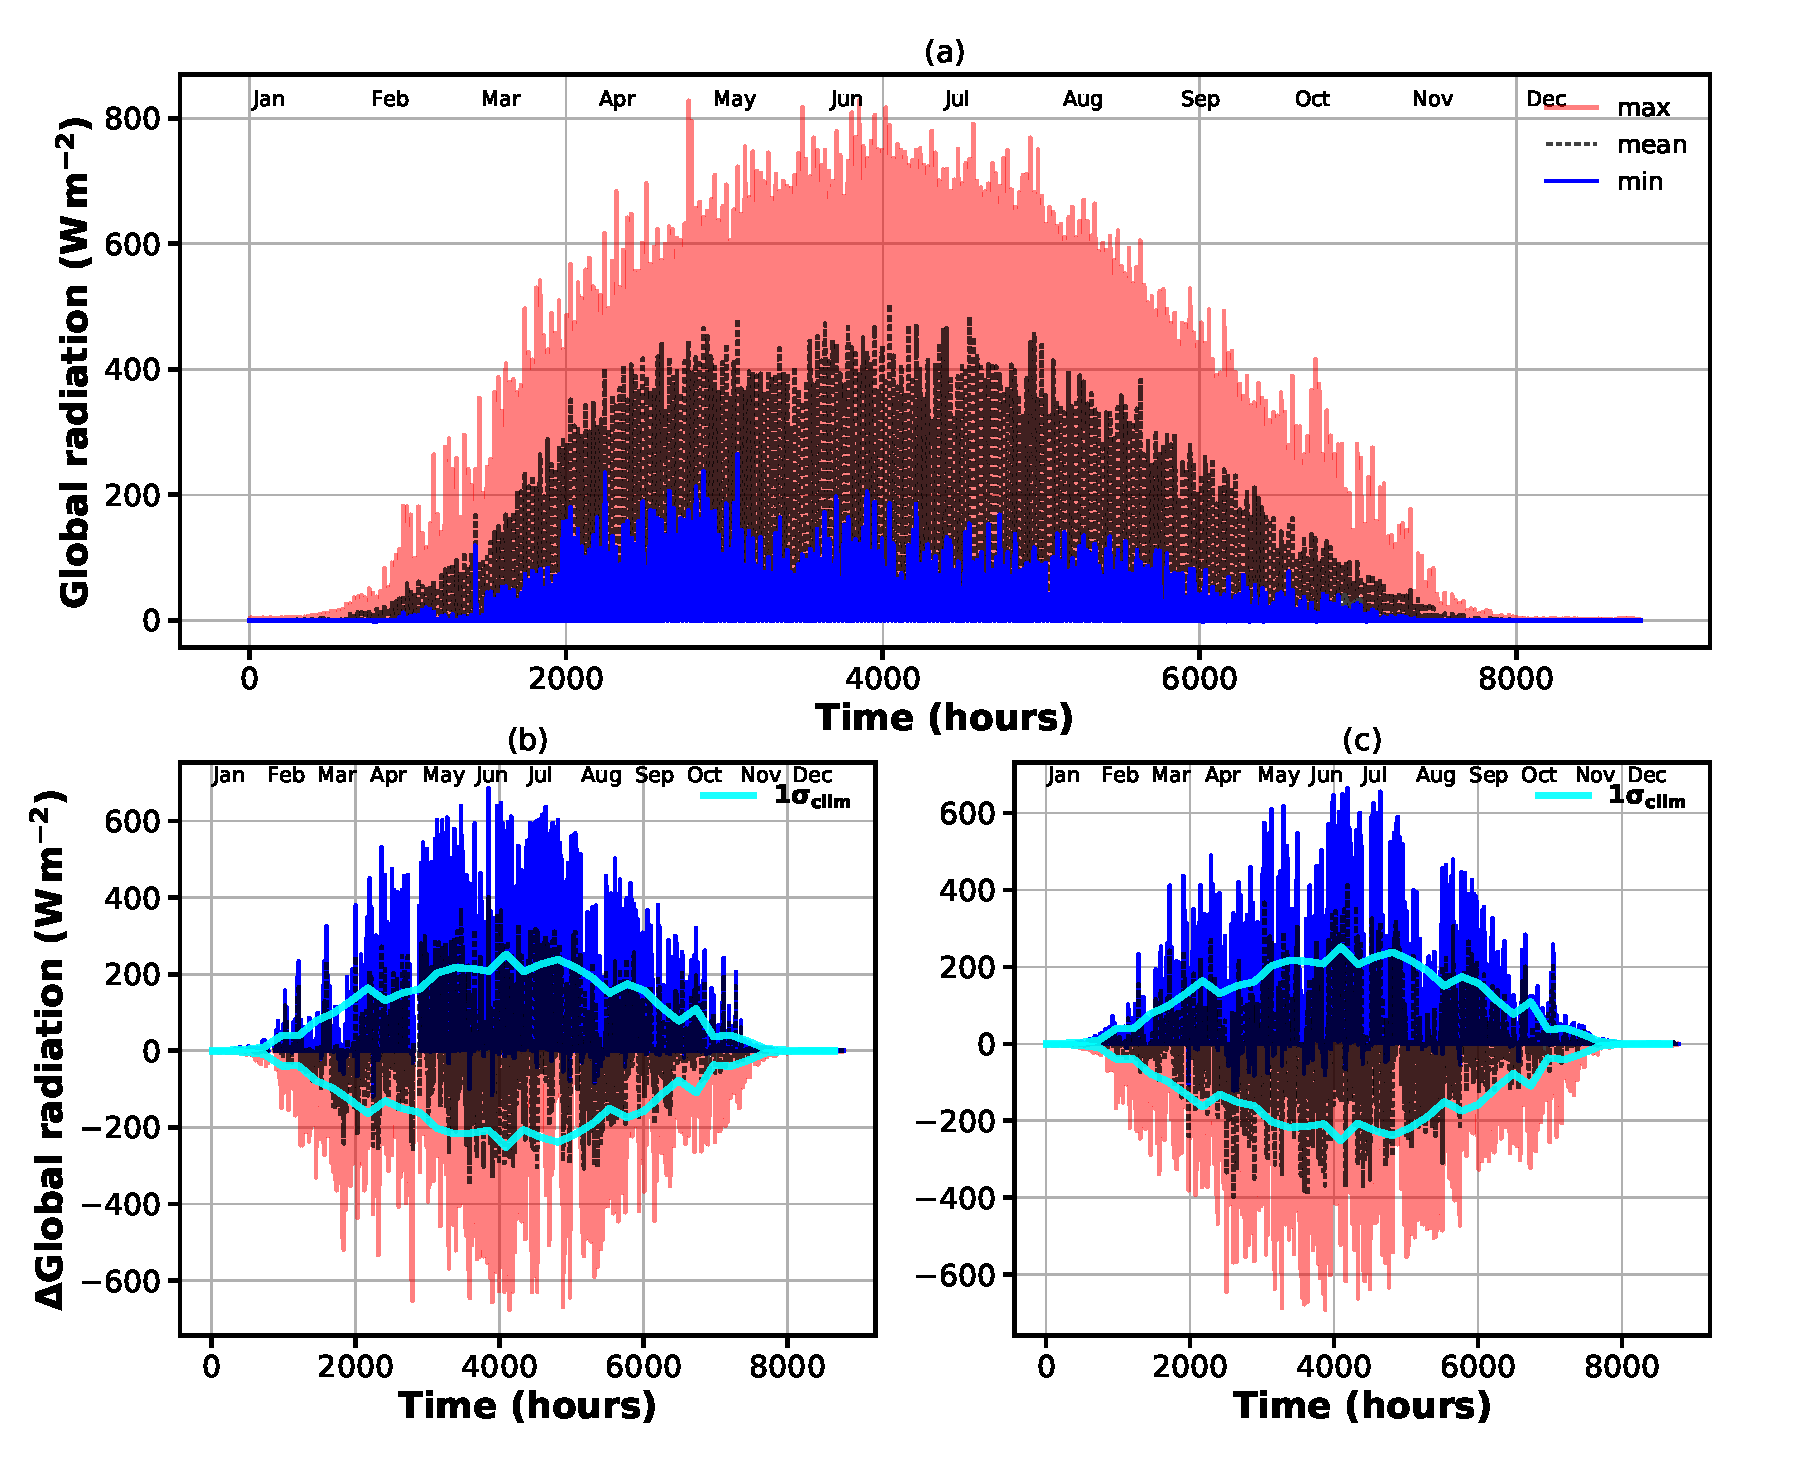
\includegraphics[width=12cm]{figA1}
  \caption{Observed global irradiance at Svanvik. (a) Climatology (hourly maxima, mean, and minima); deviation from climatology (b) 2018; (c) 2019. The cyan lines indicate the $1\,\sigma$ level derived from climatology.}
  \label{fig:global_rad_clim}
\end{figure*}

\begin{figure*}[t]
  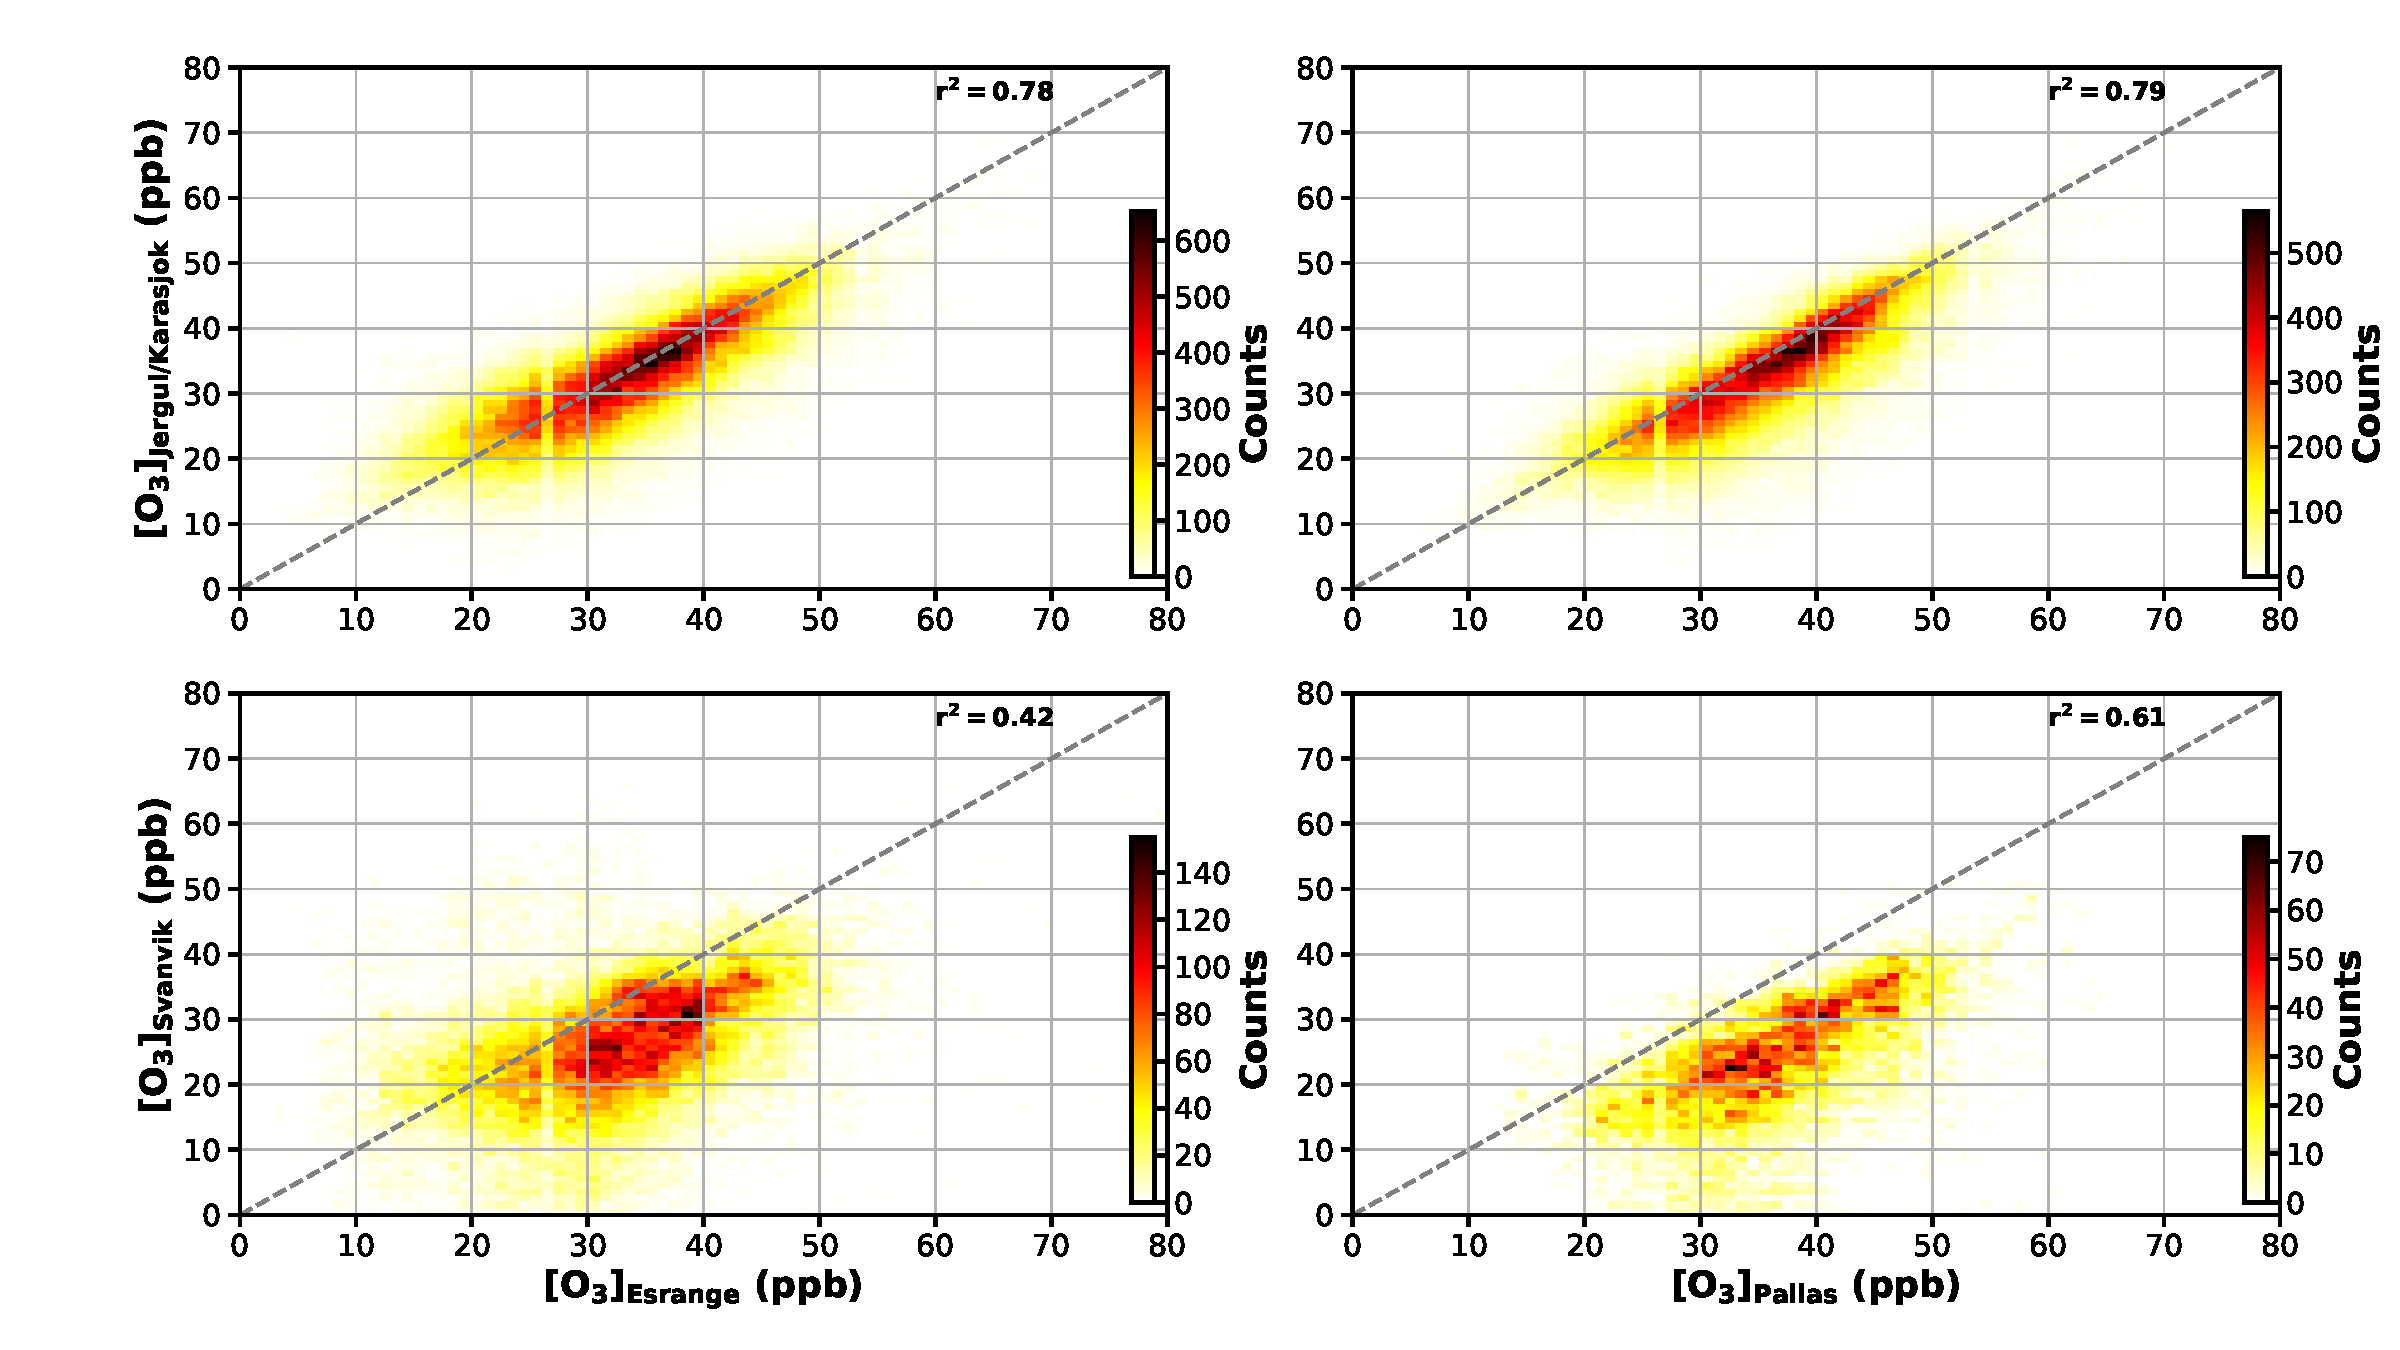
\includegraphics[width=12cm]{figA2}
  \caption{Probability densities and correlation coefficient for \chem{[O_3]} between different sites in northern Fennoscandia. Jergul/Karasjok is well correlated with Esrange, and Pallas. Svanvik displays highest correlation with Pallas. Note: The stripe at $26\,\unit{ppb}$ is an artifact from plotting. (a) Jergul/Karasjok--Esrange; (b) Jergul/Karasjok--Pallas; (c) Svanvik--Esrange; (d) Svanvik--Pallas.}
  \label{fig:density_distribution}
\end{figure*}

\begin{figure*}[t]
  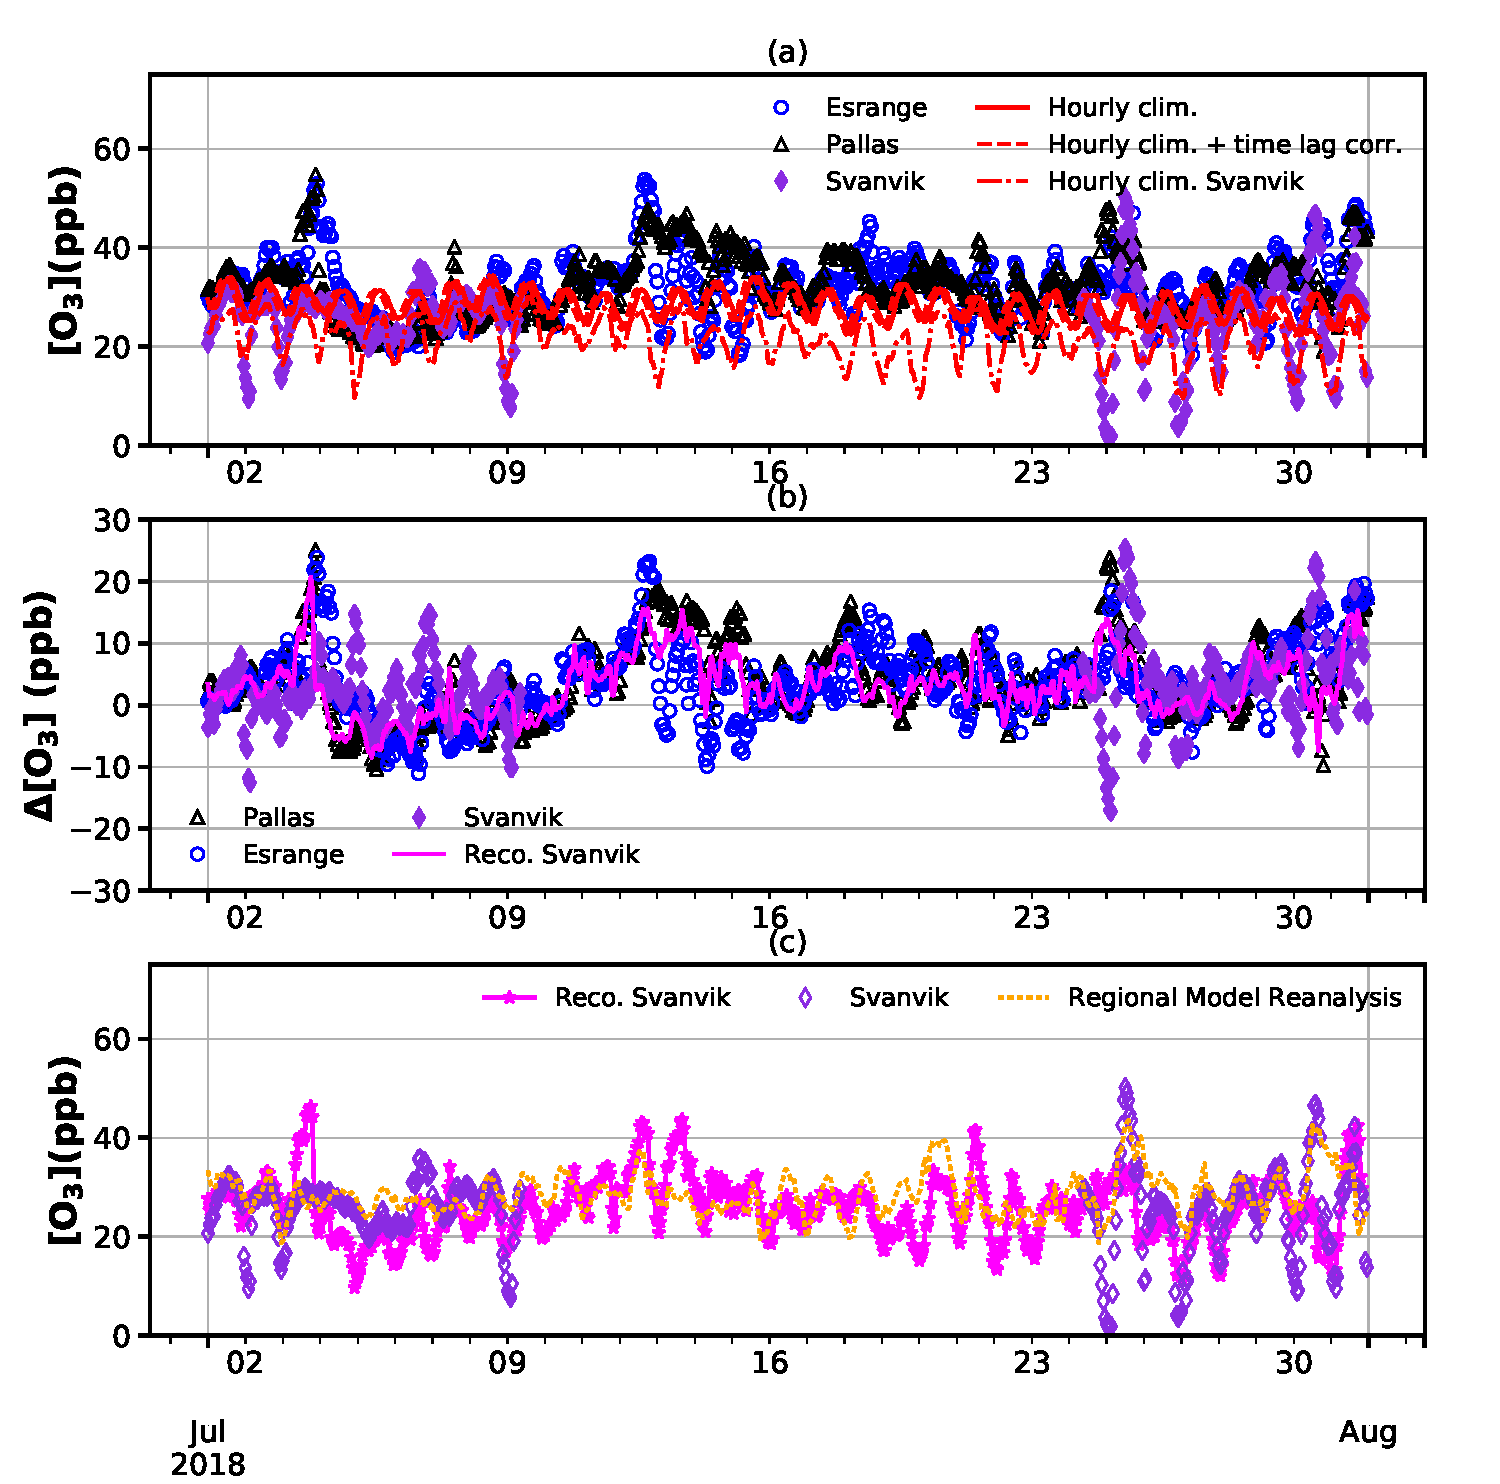
\includegraphics[width=12cm]{figA3}
  \caption{Reconstruction of missing \chem{[O_3]} observation data at Svanvik in July 2018 based on derived hourly climatologies of northern Fennoscandia, Svanvik, and data Pallas. (a) Time series; (b) anomalies; (c) reconstruction.}
  \label{fig:ozone_reconstruction_2018_07}
\end{figure*}

\clearpage

\section{DO3SE parameterization}

\begin{figure*}[t]
  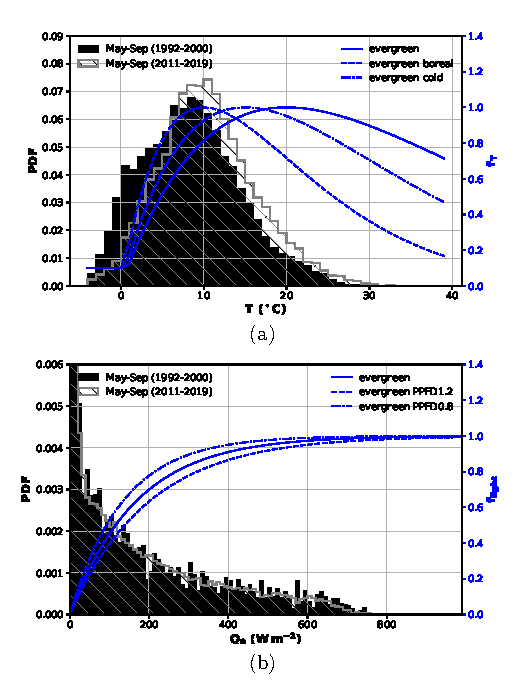
\includegraphics[width=12cm]{figB1}
  \caption{Estimated begin (BGS) and end (EGS) of growing season for coniferous trees from MODIS Aqua/Terra net photosynthesis (PSN) product. A $1\times 1\,\unit{km}$ area around Svanhovd was selected. Daily averaged data for both 2018 and 2019 has been fitted with a quadratic polynomial function. The numerically computed root yields: BGS 122/106 day of year (\unit{doy}) and EGS 261/274 day of year for 2018/2019, respectively.}
  \label{fig:modis_Psn}
\end{figure*}

\begin{figure}[t]
  %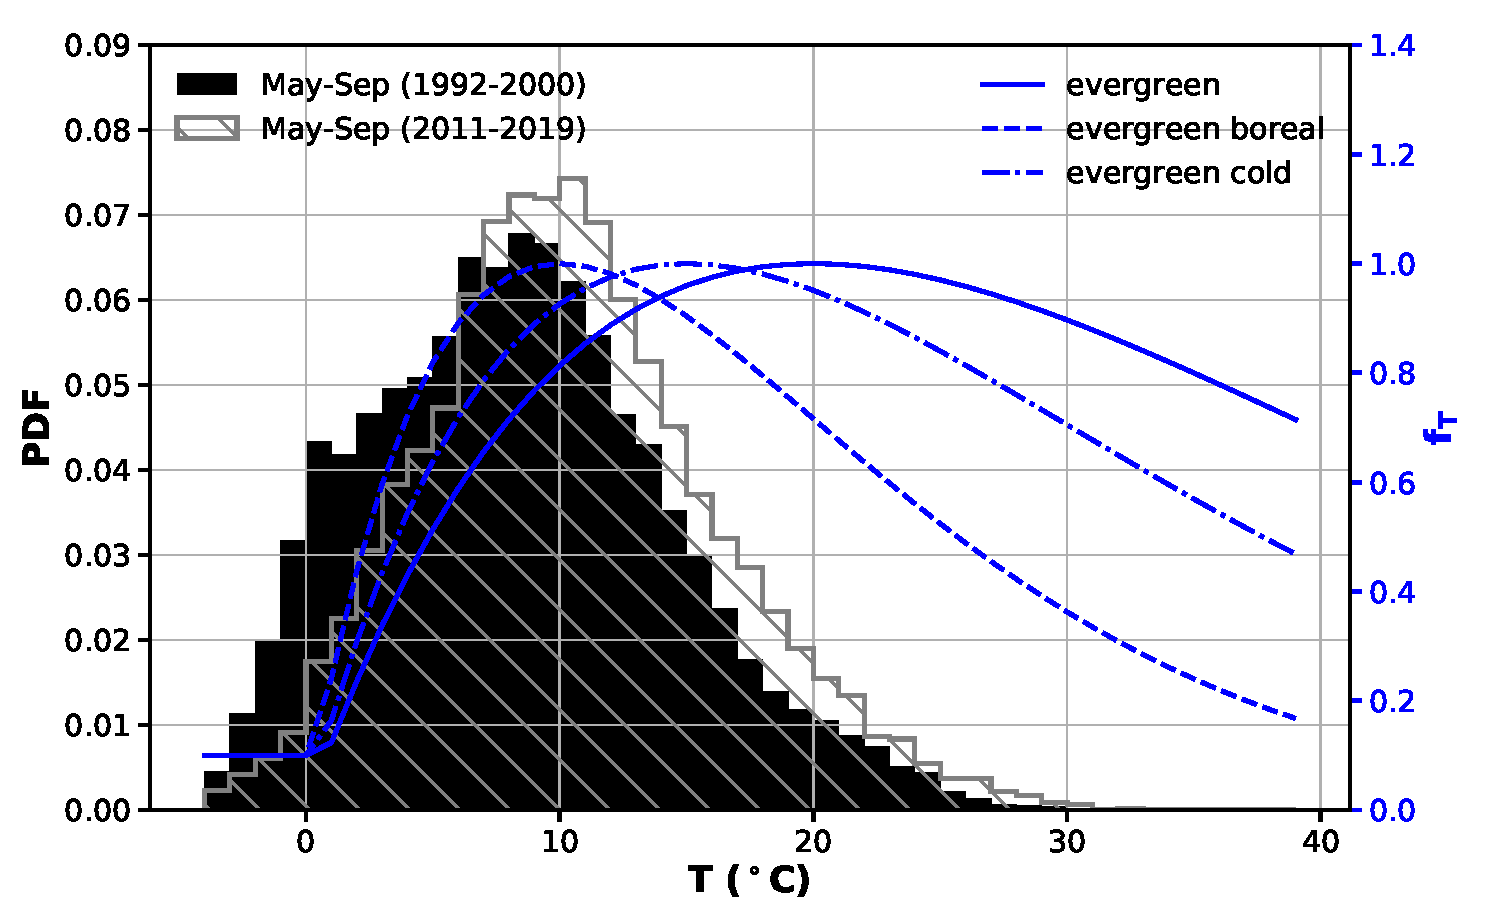
\includegraphics[width=8.3cm]{javis_funcs_temp_hist_evergreen}\\
  %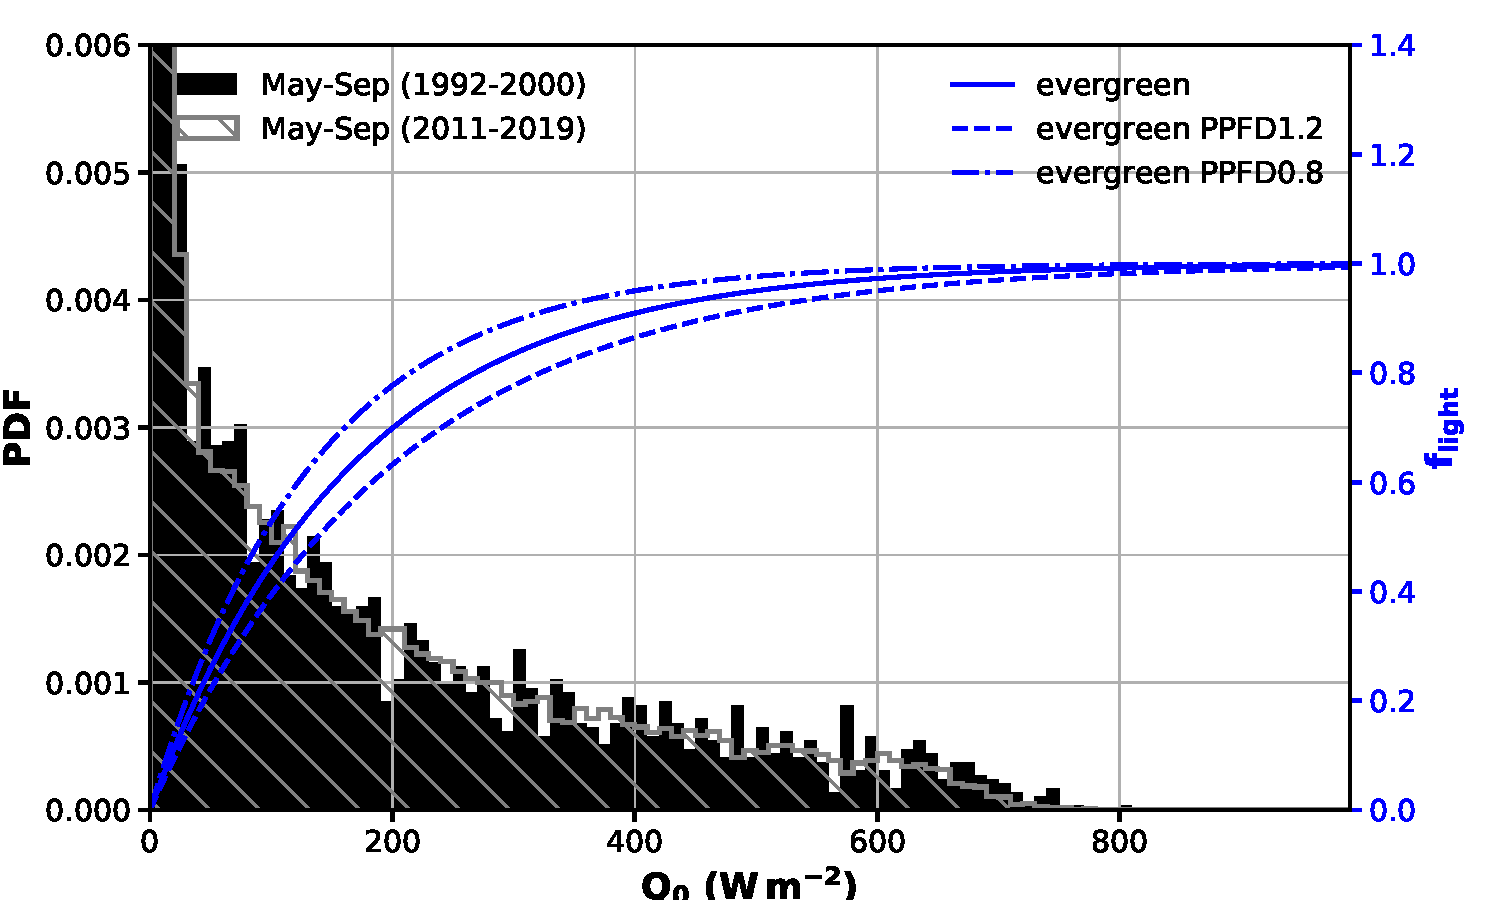
\includegraphics[width=8.3cm]{javis_funcs_rad_hist_evergreen}
  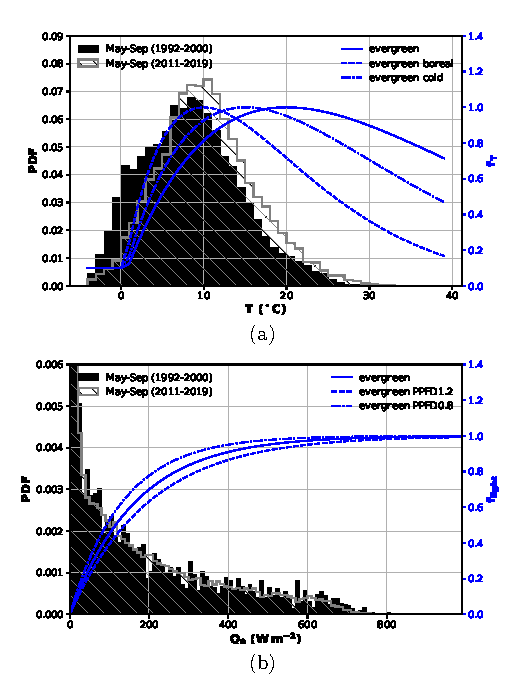
\includegraphics[width=12cm]{figB2}
\caption{Construction of bespoke response functions for Norway spruce. (a) $f_\mathrm{T}$ and (b) $f_\mathrm{flight}$ are shown together with underlying $T_\mathrm{air}$ and $Q_0$ climatologies (probability density function - PDF), respectively. Original mapping manual parameterization is shown in comparison as solid line. Note that $Q_0$ has been truncated to $0.006$. PPFD0.8 and PPFD1.2 refer to $\alpha$ values increasing/decreasing PPFD at $f_\mathrm{light}=0.5$ by $\pm 20\,\%$, respectively.}
\label{fig:f_temp_spruce}
\end{figure}

\begin{figure}[t]
  %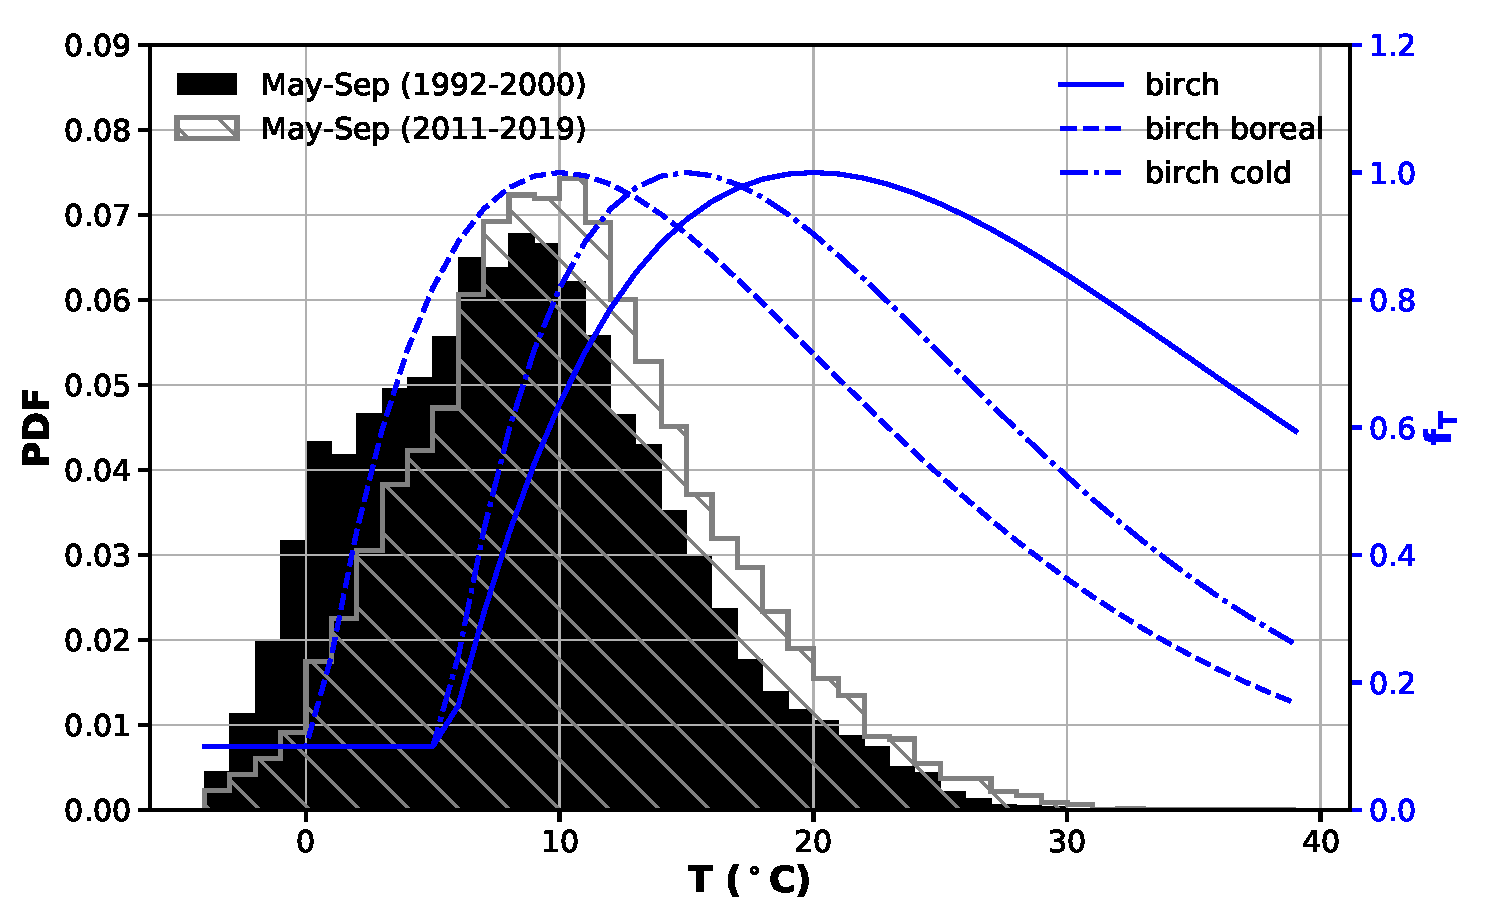
\includegraphics[width=8.3cm]{javis_funcs_temp_hist_birch}\\
  %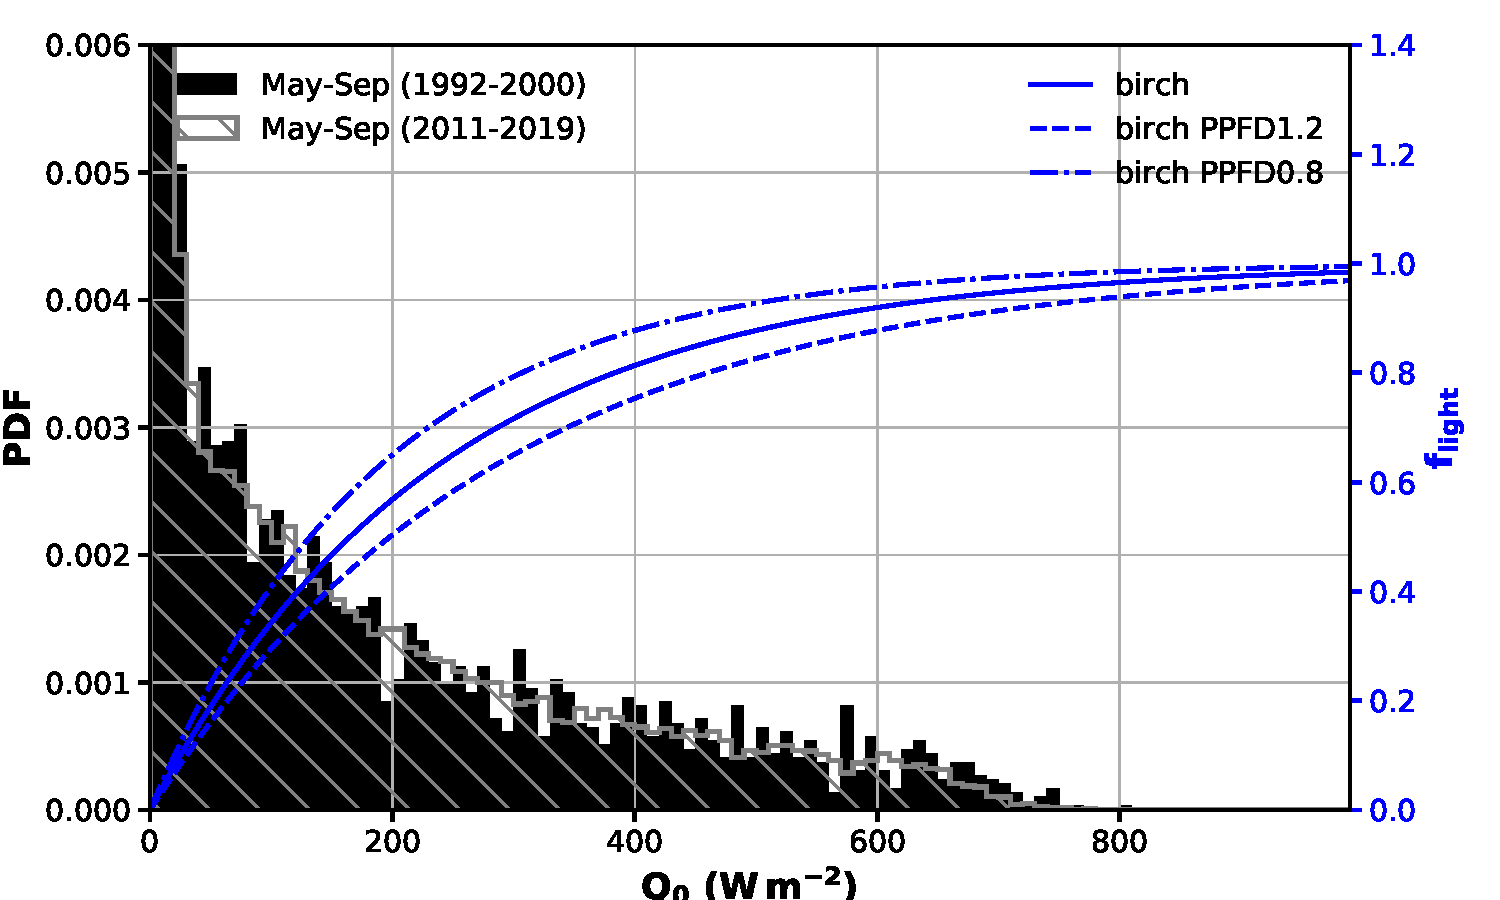
\includegraphics[width=8.3cm]{javis_funcs_rad_hist_birch}
  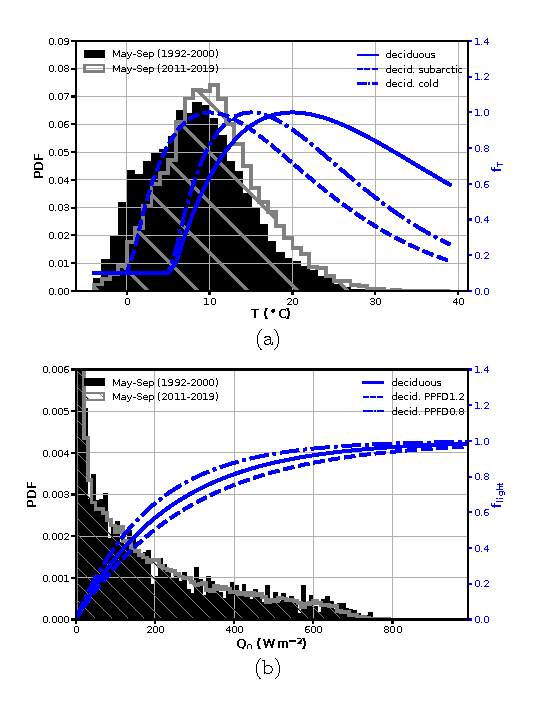
\includegraphics[width=12cm]{figB3}
\caption{Construction of bespoke response functions for downy birch. (a) $f_\mathrm{T}$ and (b) $f_\mathrm{flight}$ are shown together with underlying $T_\mathrm{air}$ and $Q_0$ climatologies (probability density function - PDF), respectively. Original mapping manual parameterization is shown in comparison as solid line. Note that $Q_0$ has been truncated to $0.006$. PPFD0.8 and PPFD1.2 refer to $\alpha$ values increasing/decreasing PPFD at $f_\mathrm{light}=0.5$ by $\pm 20\,\%$, respectively.}
\label{fig:f_temp_birch}
\end{figure}

\begin{figure*}[t]
  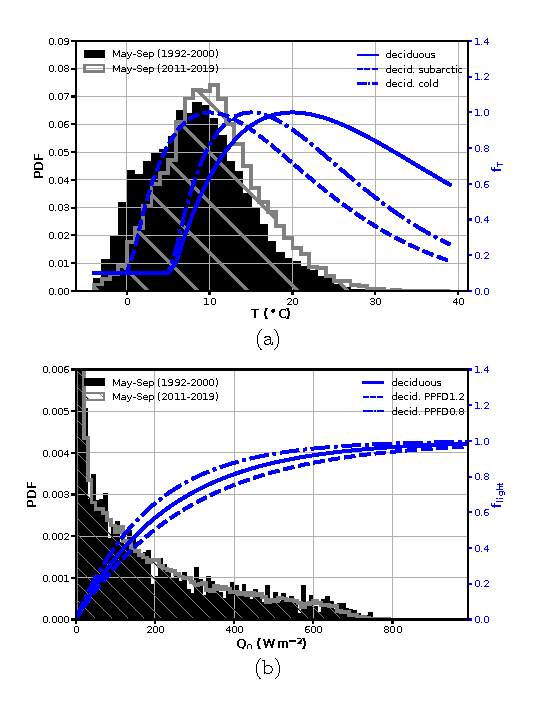
\includegraphics[width=12cm]{figB4}
  \caption{$\mathrm{DO_3SE}$ modeling results for mapping manual default parameterization. $\mathrm{POD_y}$ is shown over day of year (\unit{doy}), March--October. A flux threshold $y=1\,\unit{nmol\,m^{-2}\,s^{-1}}$ per projected leaf area (PLA) has been chosen. \chem{[O_3]} are plotted on the same axis and scales as $G_\text{sto}^\text{leaf}$ but in units of $\unit{ppb}$. (a, b) Downy birch; (c, d) Norway spruce; (e, f) perennial grassland. From left to right: 2018, 2019.}
  \label{fig:pody_mm_composit}
\end{figure*}


\noappendix       %% use this to mark the end of the appendix section. Otherwise the figures might be numbered incorrectly (e.g. 10 instead of 1).

%% Regarding figures and tables in appendices, the following two options are possible depending on your general handling of figures and tables in the manuscript environment:

%% Option 1: If you sorted all figures and tables into the sections of the text, please also sort the appendix figures and appendix tables into the respective appendix sections.
%% They will be correctly named automatically.

%% Option 2: If you put all figures after the reference list, please insert appendix tables and figures after the normal tables and figures.
%% To rename them correctly to A1, A2, etc., please add the following commands in front of them:

%\appendixfigures  %% needs to be added in front of appendix figures


%\noappendix

%\appendixtables   %% needs to be added in front of appendix tables

%% Please add \clearpage between each table and/or figure. Further guidelines on figures and tables can be found below.



\authorcontribution{SF has written the manuscript, collected and processed ozone and environmental data, and performed all statistical analyses. AVV contributed to framing this research article, has performed the on-site observation of vegetation damage induced by ozone, and advision in plant physiological processes. LE has contributed to framing of the this article, $\mathrm{DO_3SE}$ modeling, and development of the PDF-based temperature acclimation. CO has collected species or PFT parameters from literature, performed all $\mathrm{DO_3SE}$ simulations and initial validation of the results. AE contributed with her experience regarding subarctic vegetation in Finnmark. FS contributed with an assessment of the 2018 meteorological conditions. TB gave guidance in a broader research sense. All authors contributed to discussions, writing, and conclusions.} %% this section is mandatory

\competinginterests{The authors declare that they have no conflict of interest.} %% this section is mandatory even if you declare that no competing interests are present

%\disclaimer{TEXT} %% optional section

\begin{acknowledgements}
  Bj{\o}rg Rognerud for processing SeNorge.no data with respect for begin of growing season.
  Tore Flatlandsmo Berglen for hourly pressure data from Svanhovd.
  This work was financed by the Research Council of Norway (NRC) grand No. 268073.
\end{acknowledgements}




%% REFERENCES

%% The reference list is compiled as follows:

%\begin{thebibliography}{}

%\bibitem[AUTHOR(YEAR)]{LABEL1}
%REFERENCE 1

%\bibitem[AUTHOR(YEAR)]{LABEL2}
%REFERENCE 2

%\end{thebibliography}

%% Since the Copernicus LaTeX package includes the BibTeX style file copernicus.bst,
%% authors experienced with BibTeX only have to include the following two lines:
%%
\bibliographystyle{copernicus}
\bibliography{atmo.bib}
%%
%% URLs and DOIs can be entered in your BibTeX file as:
%%
%% URL = {http://www.xyz.org/~jones/idx_g.htm}
%% DOI = {10.5194/xyz}


%% LITERATURE CITATIONS
%%
%% command                        & example result
%% \citet{jones90}|               & Jones et al. (1990)
%% \citep{jones90}|               & (Jones et al., 1990)
%% \citep{jones90,jones93}|       & (Jones et al., 1990, 1993)
%% \citep[p.~32]{jones90}|        & (Jones et al., 1990, p.~32)
%% \citep[e.g.,][]{jones90}|      & (e.g., Jones et al., 1990)
%% \citep[e.g.,][p.~32]{jones90}| & (e.g., Jones et al., 1990, p.~32)
%% \citeauthor{jones90}|          & Jones et al.
%% \citeyear{jones90}|            & 1990



%% LITERATURE CITATIONS
%%
%% command                        & example result
%% \citet{jones90}|               & Jones et al. (1990)
%% \citep{jones90}|               & (Jones et al., 1990)
%% \citep{jones90,jones93}|       & (Jones et al., 1990, 1993)
%% \citep[p.~32]{jones90}|        & (Jones et al., 1990, p.~32)
%% \citep[e.g.,][]{jones90}|      & (e.g., Jones et al., 1990)
%% \citep[e.g.,][p.~32]{jones90}| & (e.g., Jones et al., 1990, p.~32)
%% \citeauthor{jones90}|          & Jones et al.
%% \citeyear{jones90}|            & 1990



%% FIGURES

%% When figures and tables are placed at the end of the MS (article in one-column style), please add \clearpage
%% between bibliography and first table and/or figure as well as between each table and/or figure.

% The figure files should be labelled correctly with Arabic numerals (e.g. fig01.jpg, fig02.png).


%% ONE-COLUMN FIGURES

%%f
%\begin{figure}[t]
%\includegraphics[width=8.3cm]{FILE NAME}
%\caption{TEXT}
%\end{figure}
%
%%% TWO-COLUMN FIGURES
%
%%f
%\begin{figure*}[t]
%\includegraphics[width=12cm]{FILE NAME}
%\caption{TEXT}
%\end{figure*}
%
%
%%% TABLES
%%%
%%% The different columns must be seperated with a & command and should
%%% end with \\ to identify the column brake.
%
%%% ONE-COLUMN TABLE
%
%%t
%\begin{table}[t]
%\caption{TEXT}
%\begin{tabular}{column = lcr}
%\tophline
%
%\middlehline
%
%\bottomhline
%\end{tabular}
%\belowtable{} % Table Footnotes
%\end{table}
%
%%% TWO-COLUMN TABLE
%
%%t
%\begin{table*}[t]
%\caption{TEXT}
%\begin{tabular}{column = lcr}
%\tophline
%
%\middlehline
%
%\bottomhline
%\end{tabular}
%\belowtable{} % Table Footnotes
%\end{table*}
%
%%% LANDSCAPE TABLE
%
%%t
%\begin{sidewaystable*}[t]
%\caption{TEXT}
%\begin{tabular}{column = lcr}
%\tophline
%
%\middlehline
%
%\bottomhline
%\end{tabular}
%\belowtable{} % Table Footnotes
%\end{sidewaystable*}
%
%
%%% MATHEMATICAL EXPRESSIONS
%
%%% All papers typeset by Copernicus Publications follow the math typesetting regulations
%%% given by the IUPAC Green Book (IUPAC: Quantities, Units and Symbols in Physical Chemistry,
%%% 2nd Edn., Blackwell Science, available at: http://old.iupac.org/publications/books/gbook/green_book_2ed.pdf, 1993).
%%%
%%% Physical quantities/variables are typeset in italic font (t for time, T for Temperature)
%%% Indices which are not defined are typeset in italic font (x, y, z, a, b, c)
%%% Items/objects which are defined are typeset in roman font (Car A, Car B)
%%% Descriptions/specifications which are defined by itself are typeset in roman font (abs, rel, ref, tot, net, ice)
%%% Abbreviations from 2 letters are typeset in roman font (RH, LAI)
%%% Vectors are identified in bold italic font using \vec{x}
%%% Matrices are identified in bold roman font
%%% Multiplication signs are typeset using the LaTeX commands \times (for vector products, grids, and exponential notations) or \cdot
%%% The character * should not be applied as mutliplication sign
%
%
%%% EQUATIONS
%
%%% Single-row equation
%
%\begin{equation}
%
%\end{equation}
%
%%% Multiline equation
%
%\begin{align}
%& 3 + 5 = 8\\
%& 3 + 5 = 8\\
%& 3 + 5 = 8
%\end{align}
%
%
%%% MATRICES
%
%\begin{matrix}
%x & y & z\\
%x & y & z\\
%x & y & z\\
%\end{matrix}
%
%
%%% ALGORITHM
%
%\begin{algorithm}
%\caption{...}
%\label{a1}
%\begin{algorithmic}
%...
%\end{algorithmic}
%\end{algorithm}
%
%
%%% CHEMICAL FORMULAS AND REACTIONS
%
%%% For formulas embedded in the text, please use \chem{}
%
%%% The reaction environment creates labels including the letter R, i.e. (R1), (R2), etc.
%
%\begin{reaction}
%%% \rightarrow should be used for normal (one-way) chemical reactions
%%% \rightleftharpoons should be used for equilibria
%%% \leftrightarrow should be used for resonance structures
%\end{reaction}
%
%
%%% PHYSICAL UNITS
%%%
%%% Please use \unit{} and apply the exponential notation

\graphicspath{{figures_supplement/}}          % graphics
\renewcommand{\thefigure}{S\arabic{figure}}
\renewcommand{\thetable}{S\arabic{table}}

\clearpage
\setcounter{page}{1}
\setcounter{section}{1}
\setcounter{figure}{0}

\section*{Supplement}

\begin{figure*}[th]
  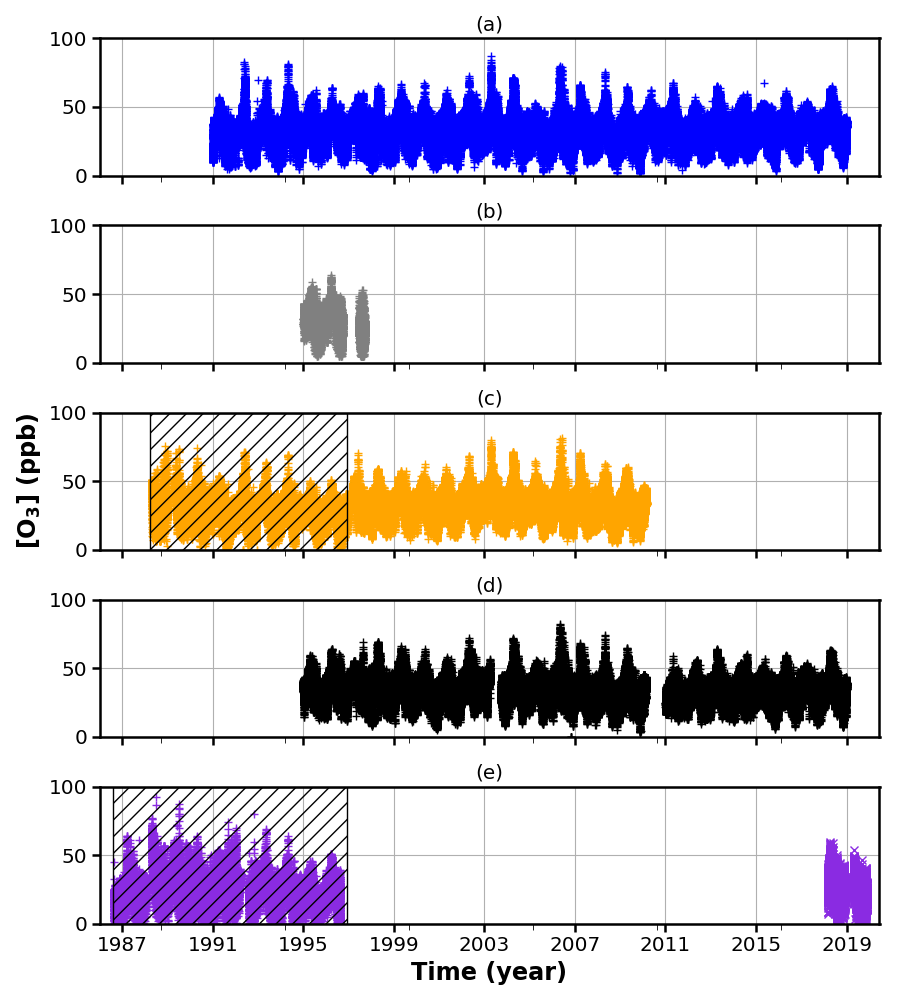
\includegraphics[width=12cm]{ozone_timeseries_fennoscandic_obs.png}
  \caption{Time series of ozone observations in northern Fennoscandia (Tab.~\ref{tab:ebas_obs}) (1986--2019). Data from EBAS until December 2018. The hatched areas indicate periods with insufficient quality control according to \citet{NILU2003}. (a) Esrange (SWE); (b) Janiskoski (RUS); (c) Jergul/Karasjok (NOR); (d) Pallas (FIN); (e) Svanvik (NOR).}
  \label{fig:ozone_timesseries_fenoscandic_obs}
\end{figure*}

%\begin{figure*}[t]
%  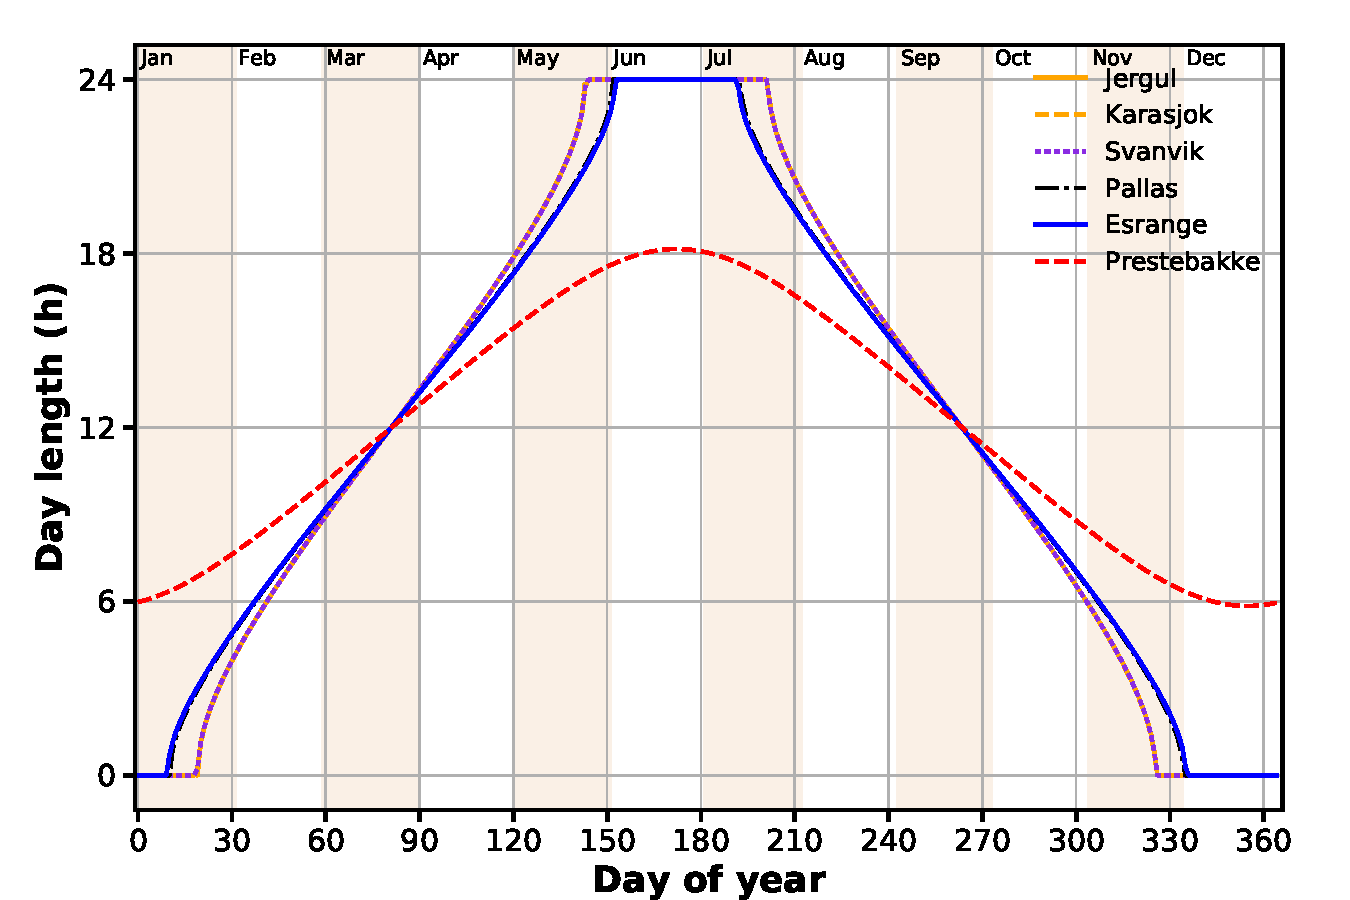
\includegraphics[width=12cm]{test_fennoscandia}
%  \caption{Maximum daily sun shine duration based on geometrical calculations at different sites in Fennoscandia. Midnight sun conditions at Jergul/Karasjok and Svanvik prevail from the end of May until the end of July, while at Esrange and Pallas they only prevail from the beginning of June until mid of July.}
%  \label{fig:sunlight_fennoscandia}
%\end{figure*}

%\begin{figure*}[t]
%  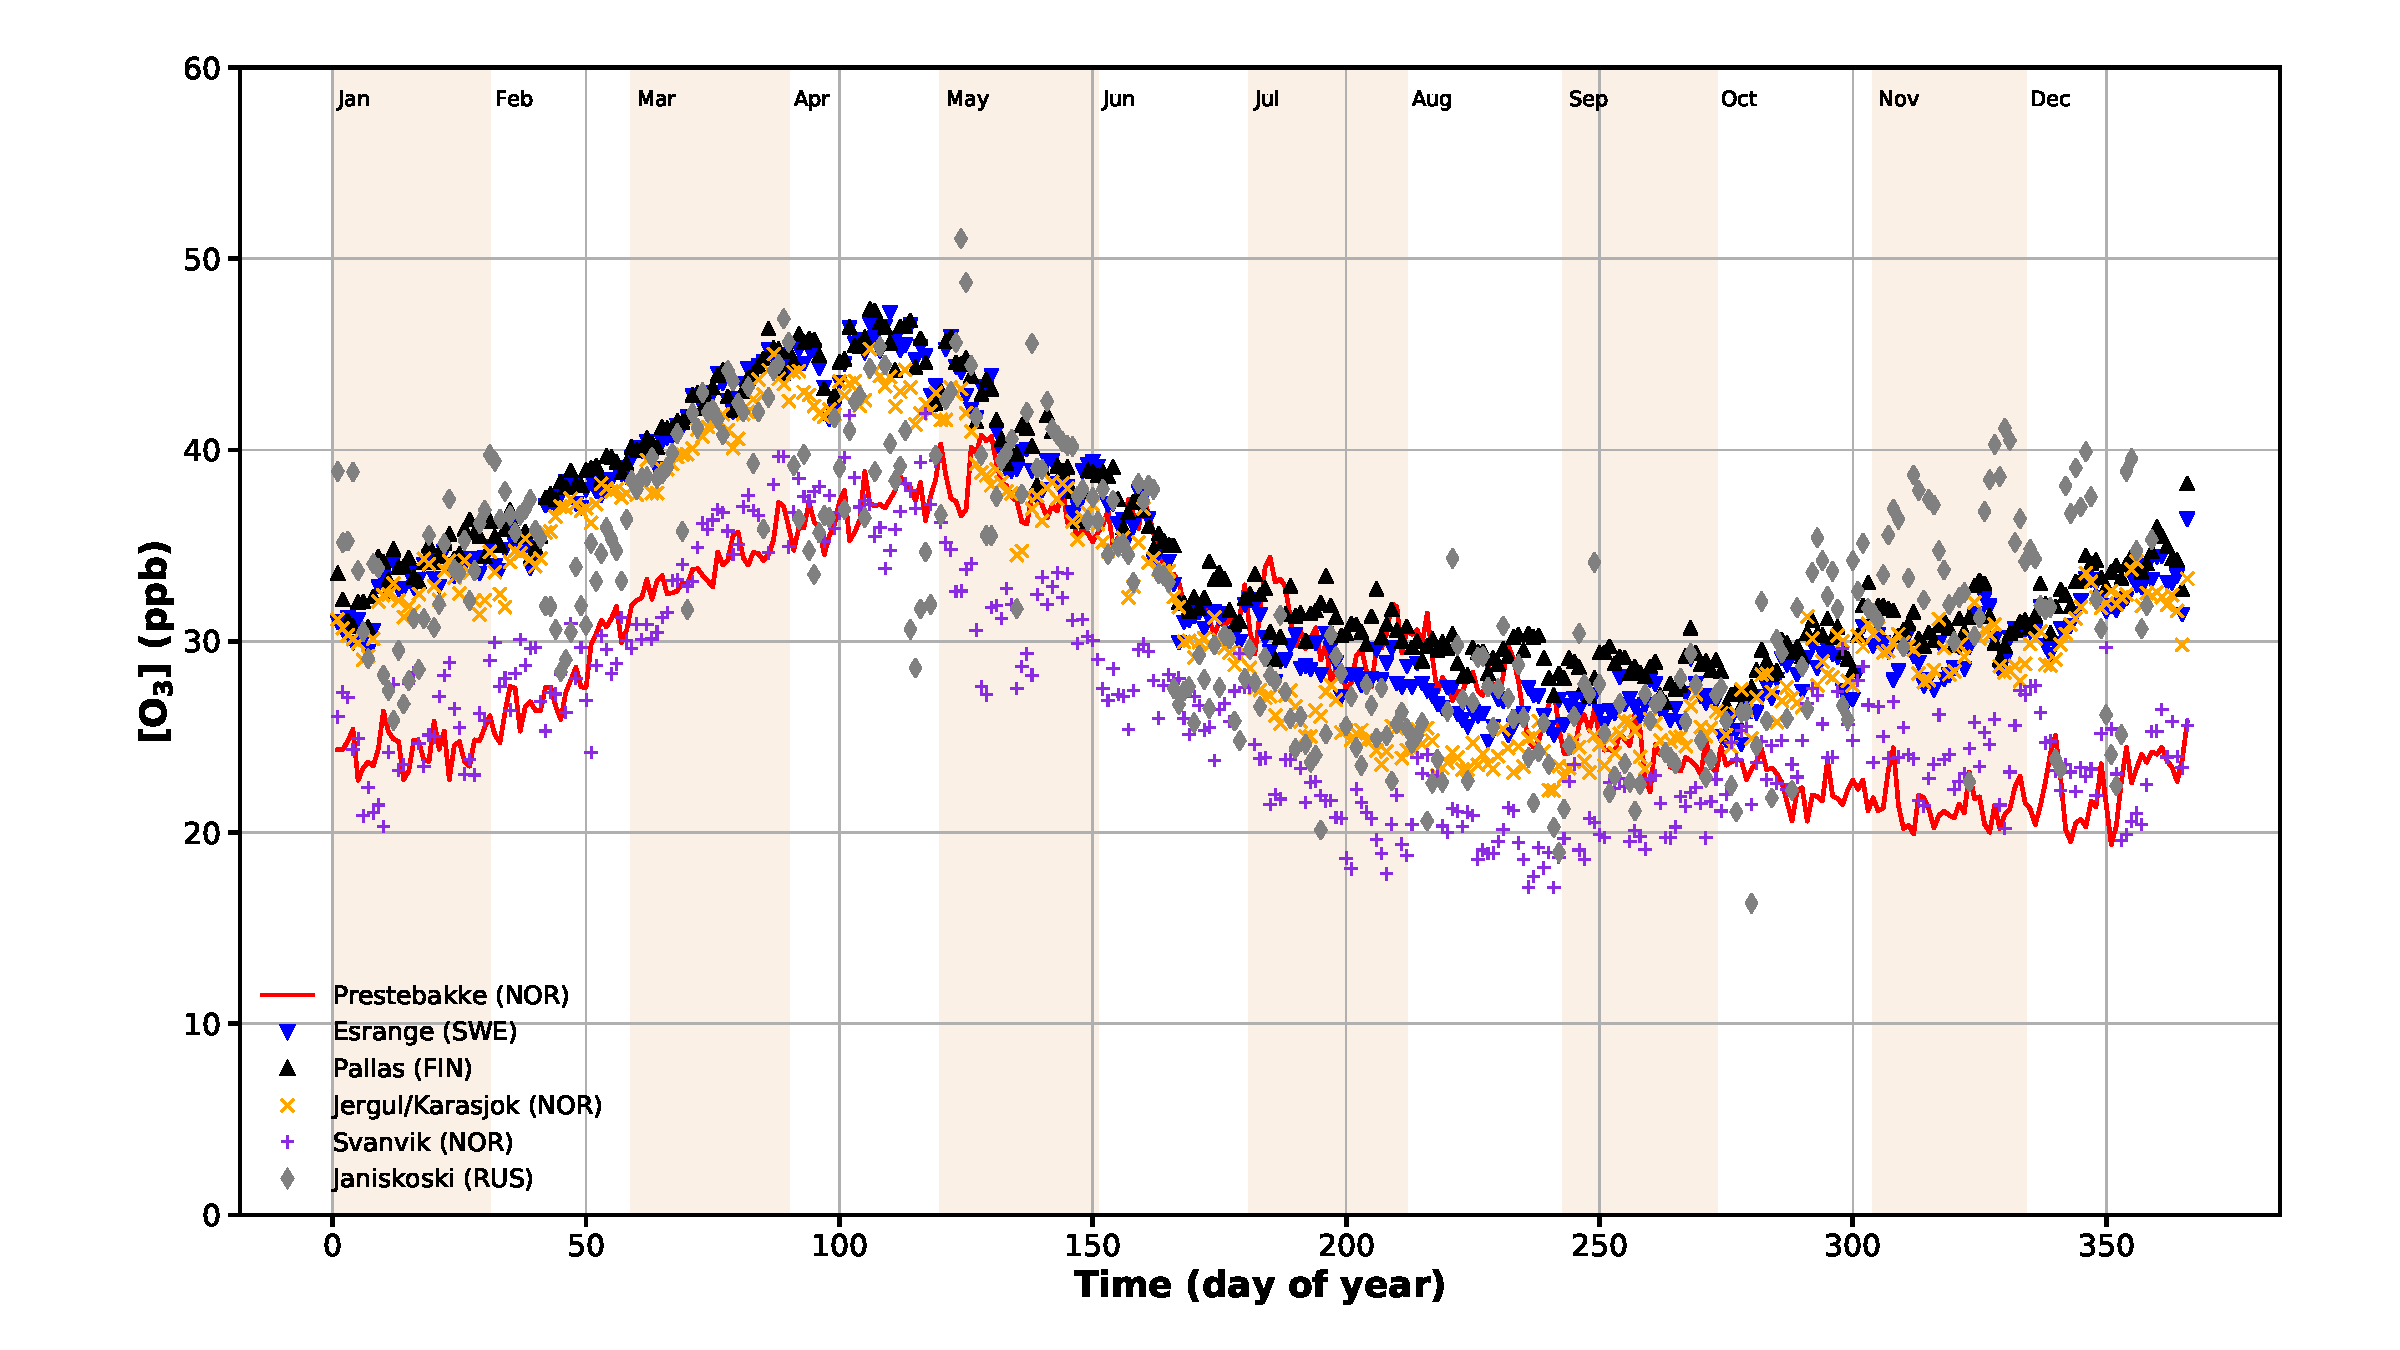
\includegraphics[width=12cm]{ozone_climatology_fenoscandic_obs}
%  \caption{Multi-annual mean of daily mean ozone at observation sites in Fennoscandia. The large spread in case of Svanvik and Janiskoski is due to the lower statistics. All climatologies peak in spring, with peak values in April. The annual average ozone concentration \chem{\left<[O_3]\right>} at Svanvik is $6.6\,\unit{ppb}$ lower than at the sites at Jergul/Karasjok (NOR), Esrange (SWE), and Pallas (FIN).}
%  \label{fig:ozone_climatology_fenoscandic_obs}
%\end{figure*}

\begin{figure*}[th]
  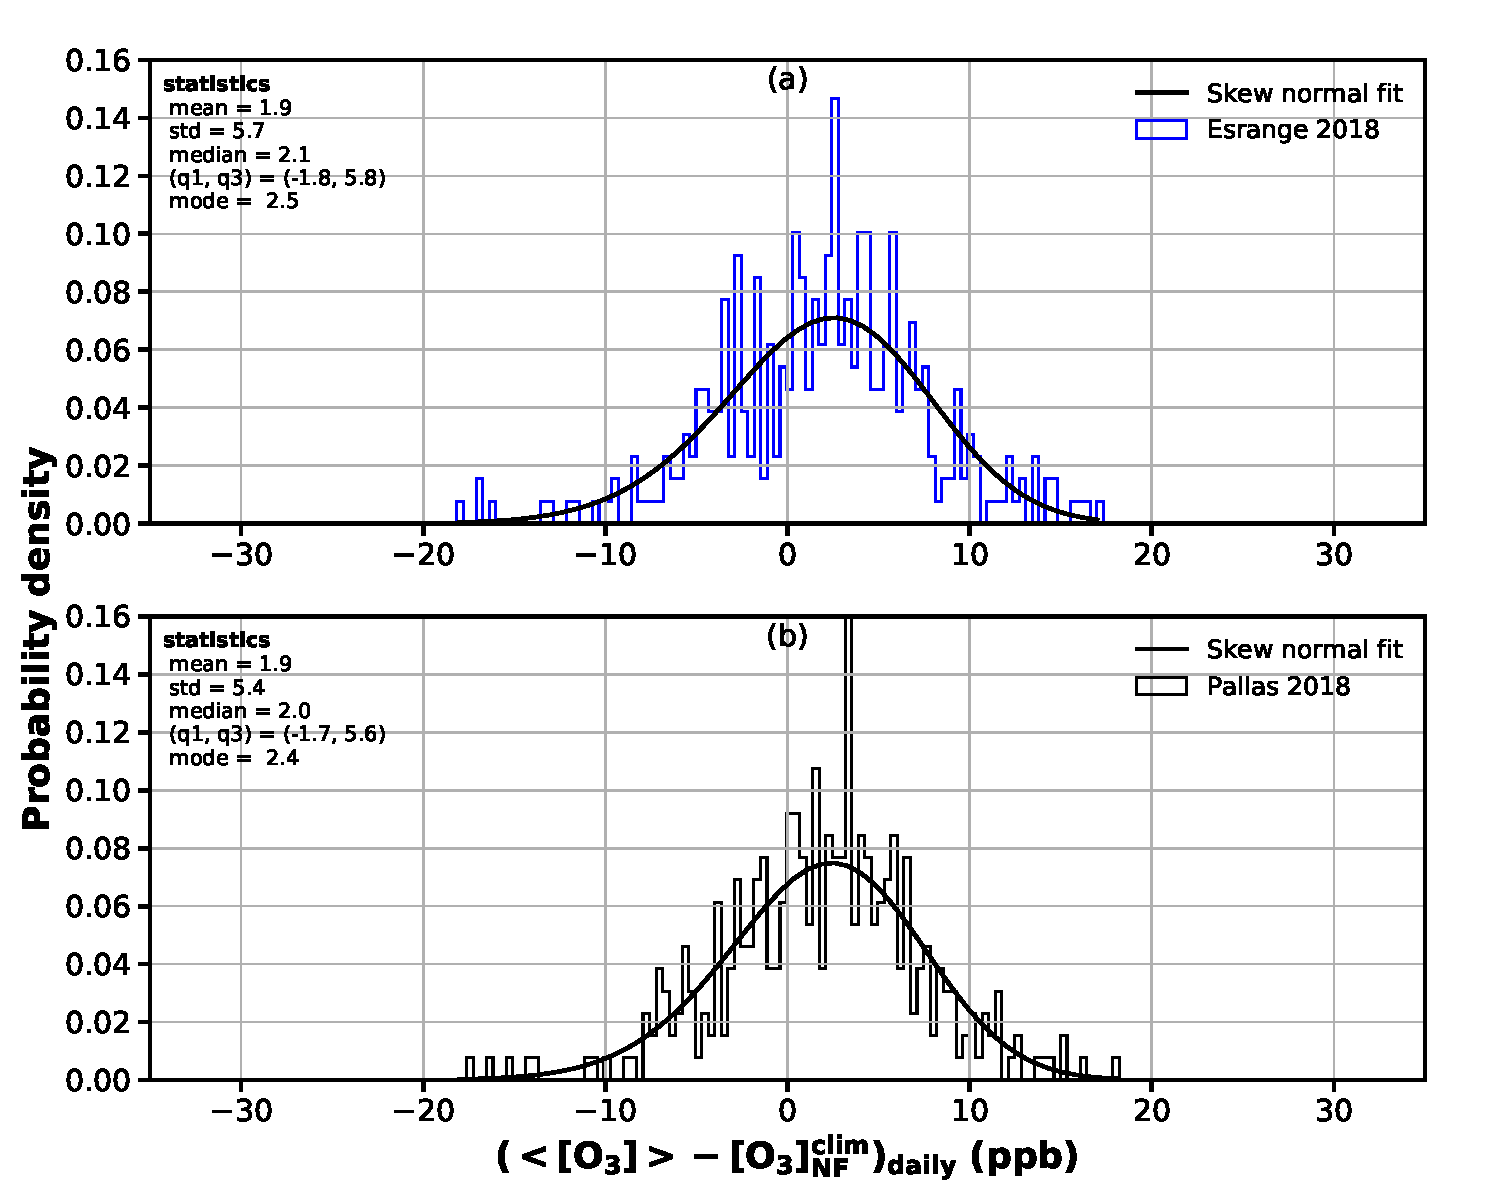
\includegraphics[width=12cm]{ozone_climatology_fenoscandic_obs_residuals}
  \caption{Probability density functions of ozone concentration residuals. 2018 with respect to respective climatology for different sites in Fennoscandia. (a) Esrange; (b) Pallas.}
  \label{fig:ozone_climatology_fenoscandic_obs_residuals}
\end{figure*}

\begin{figure*}[th]
  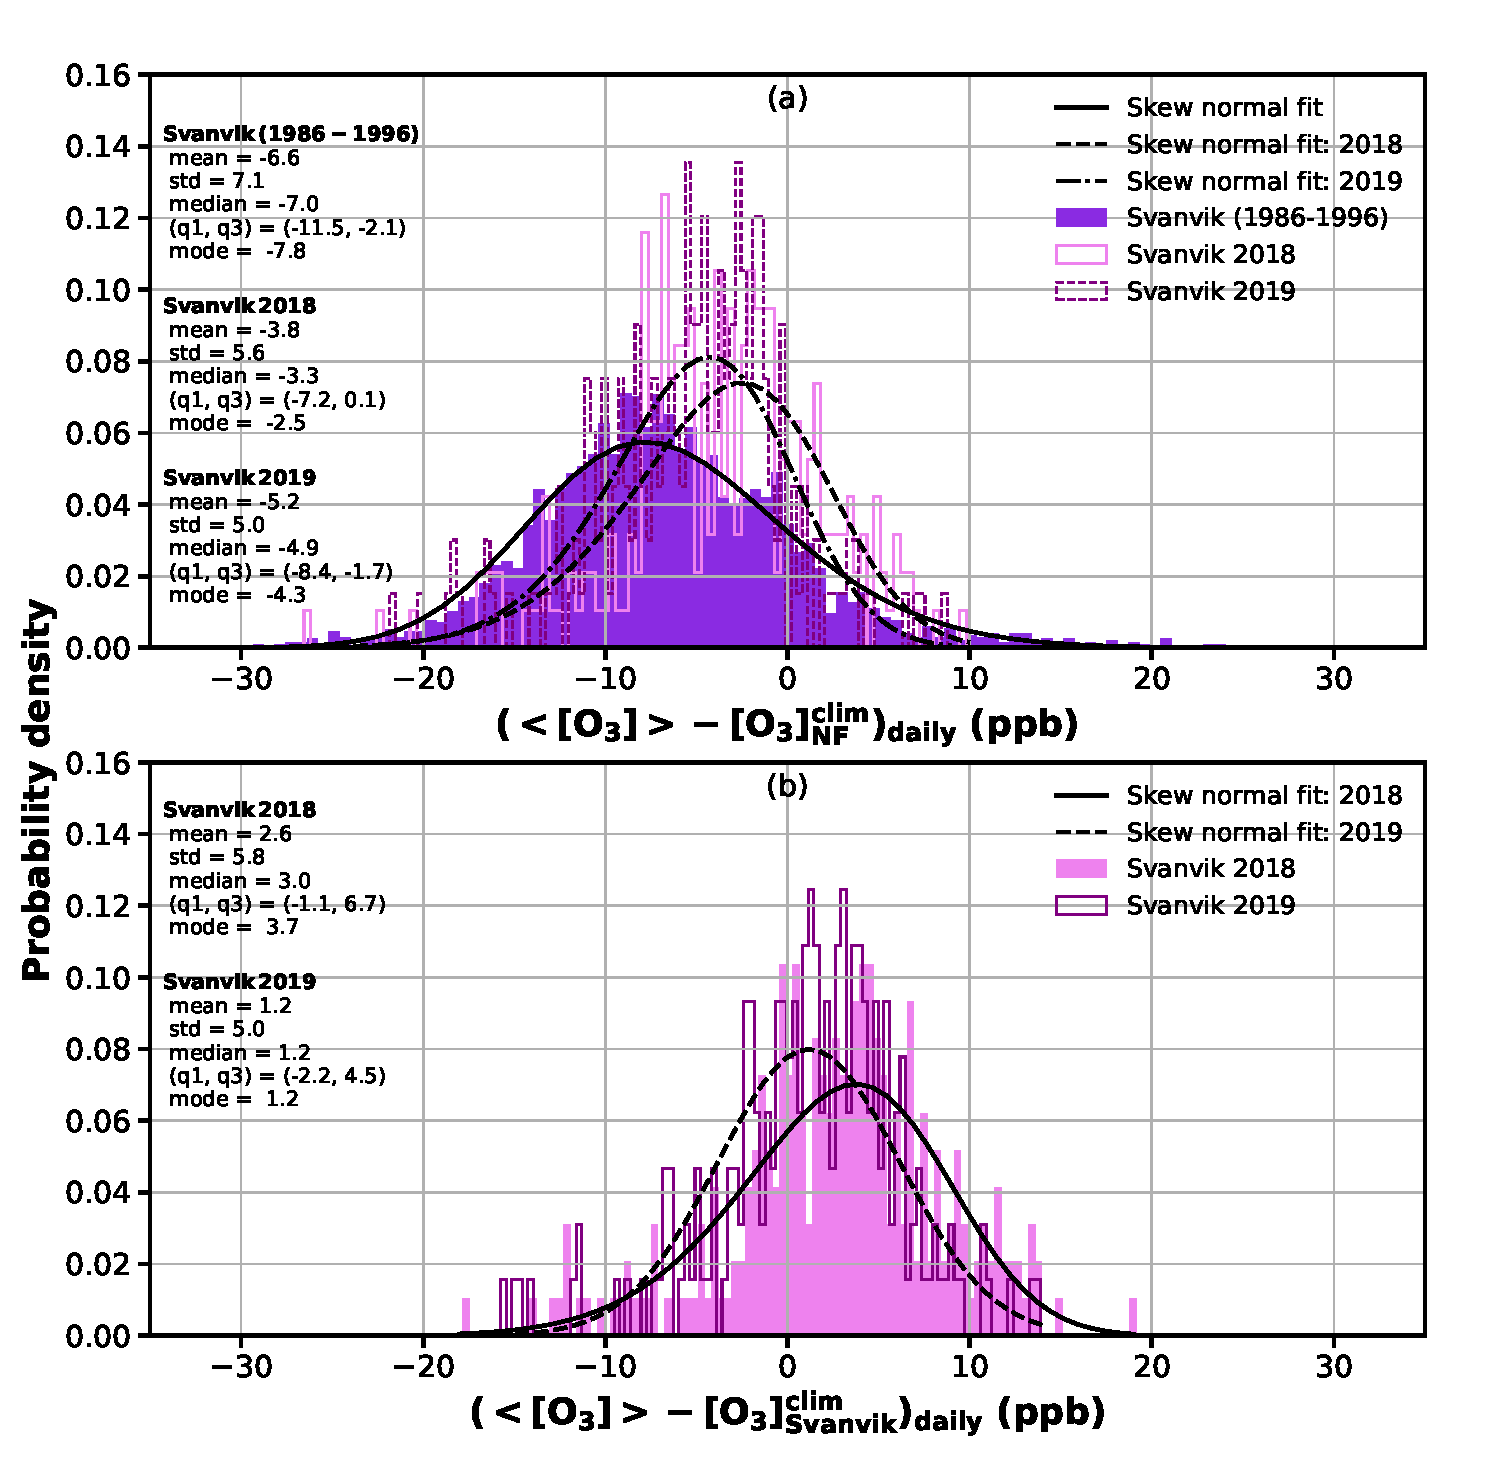
\includegraphics[width=12cm]{ozone_climatology_fenoscandic_obs_residuals-Svanvik}
  \caption{Probability density functions of ozone concentration residuals. 2018/19 observations at Svanhovd with respect to derived climatologies for (a) Northern Fennoscandia; (b) Svanvik.}
  \label{fig:ozone_climatology_fenoscandic_obs_residuals-Svanvik}
\end{figure*}

\begin{figure*}[th]
  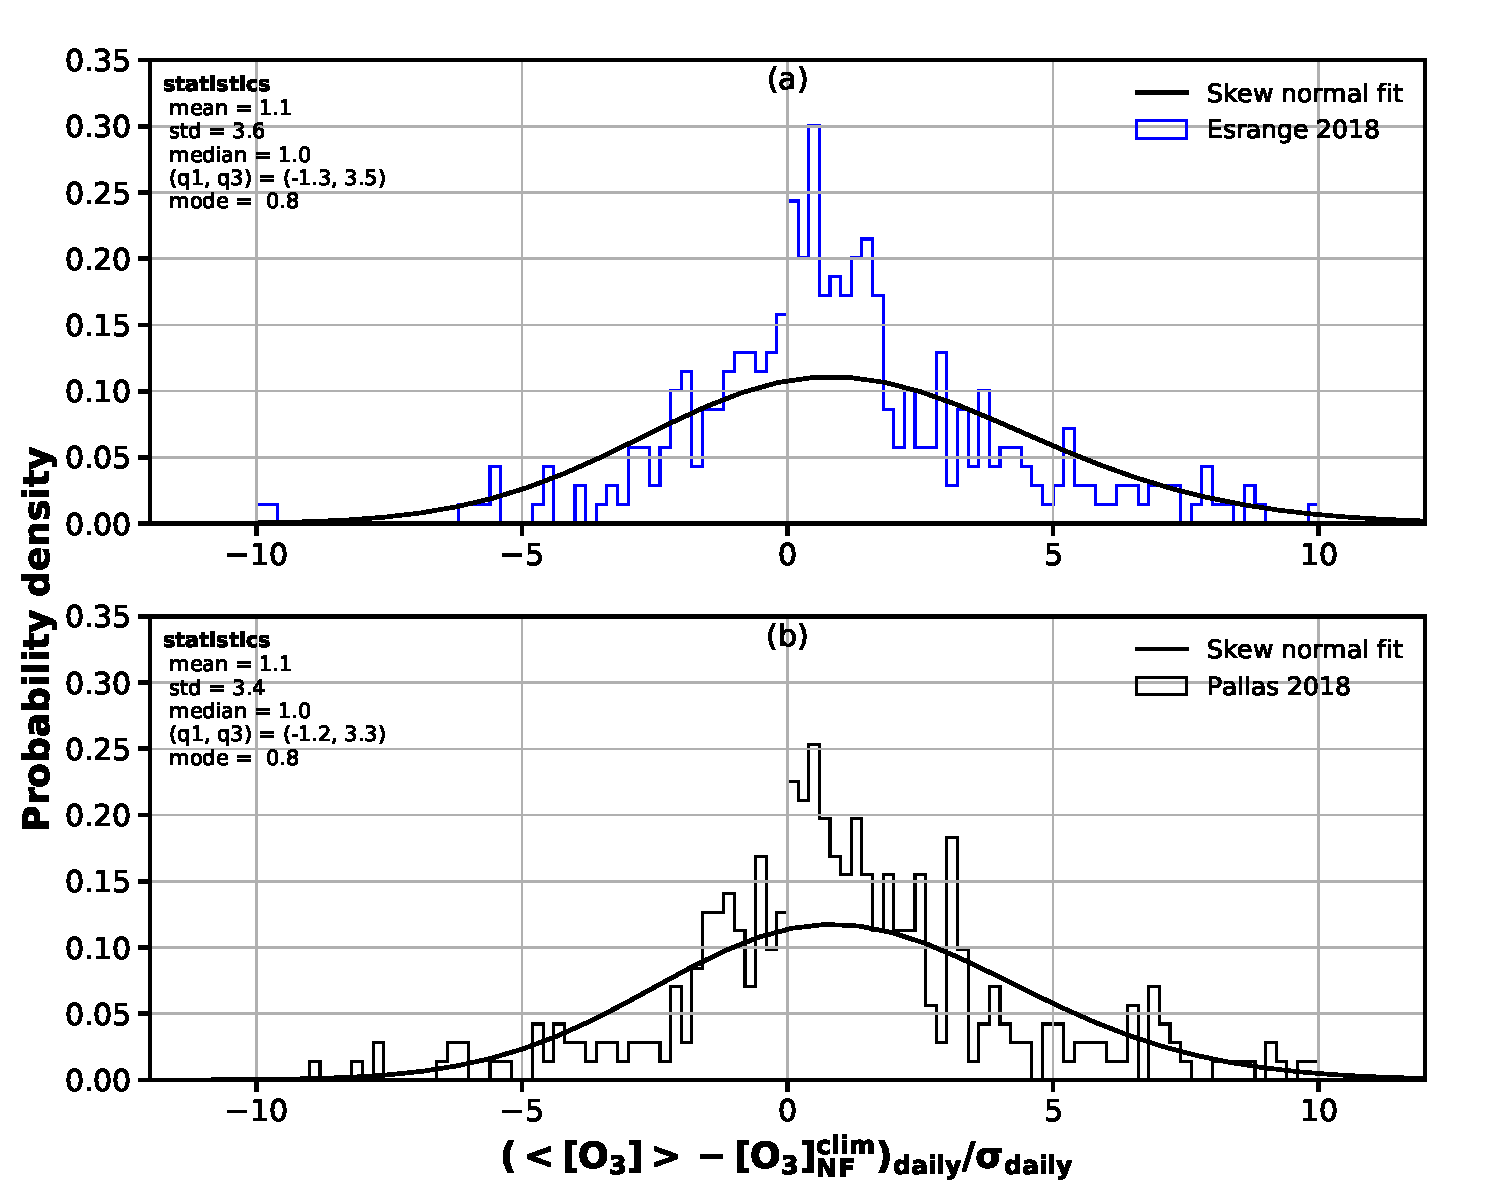
\includegraphics[width=12cm]{ozone_climatology_fenoscandic_obs_test}
  \caption{Student's t-test assuming same sample uncertainty in both, climatology and 2018 observations for different sites in Fennoscandia. \chem{\Delta[O_3]} in Fig.~\ref{fig:ozone_climatology_fenoscandic_obs_residuals} are significantly different from zero-hypothesis on the $1\,\sigma$ level. (a) Esrange; (b) Pallas.}
  \label{fig:ozone_climatology_fenoscandic_obs_test}
\end{figure*}

\begin{figure*}[th]
  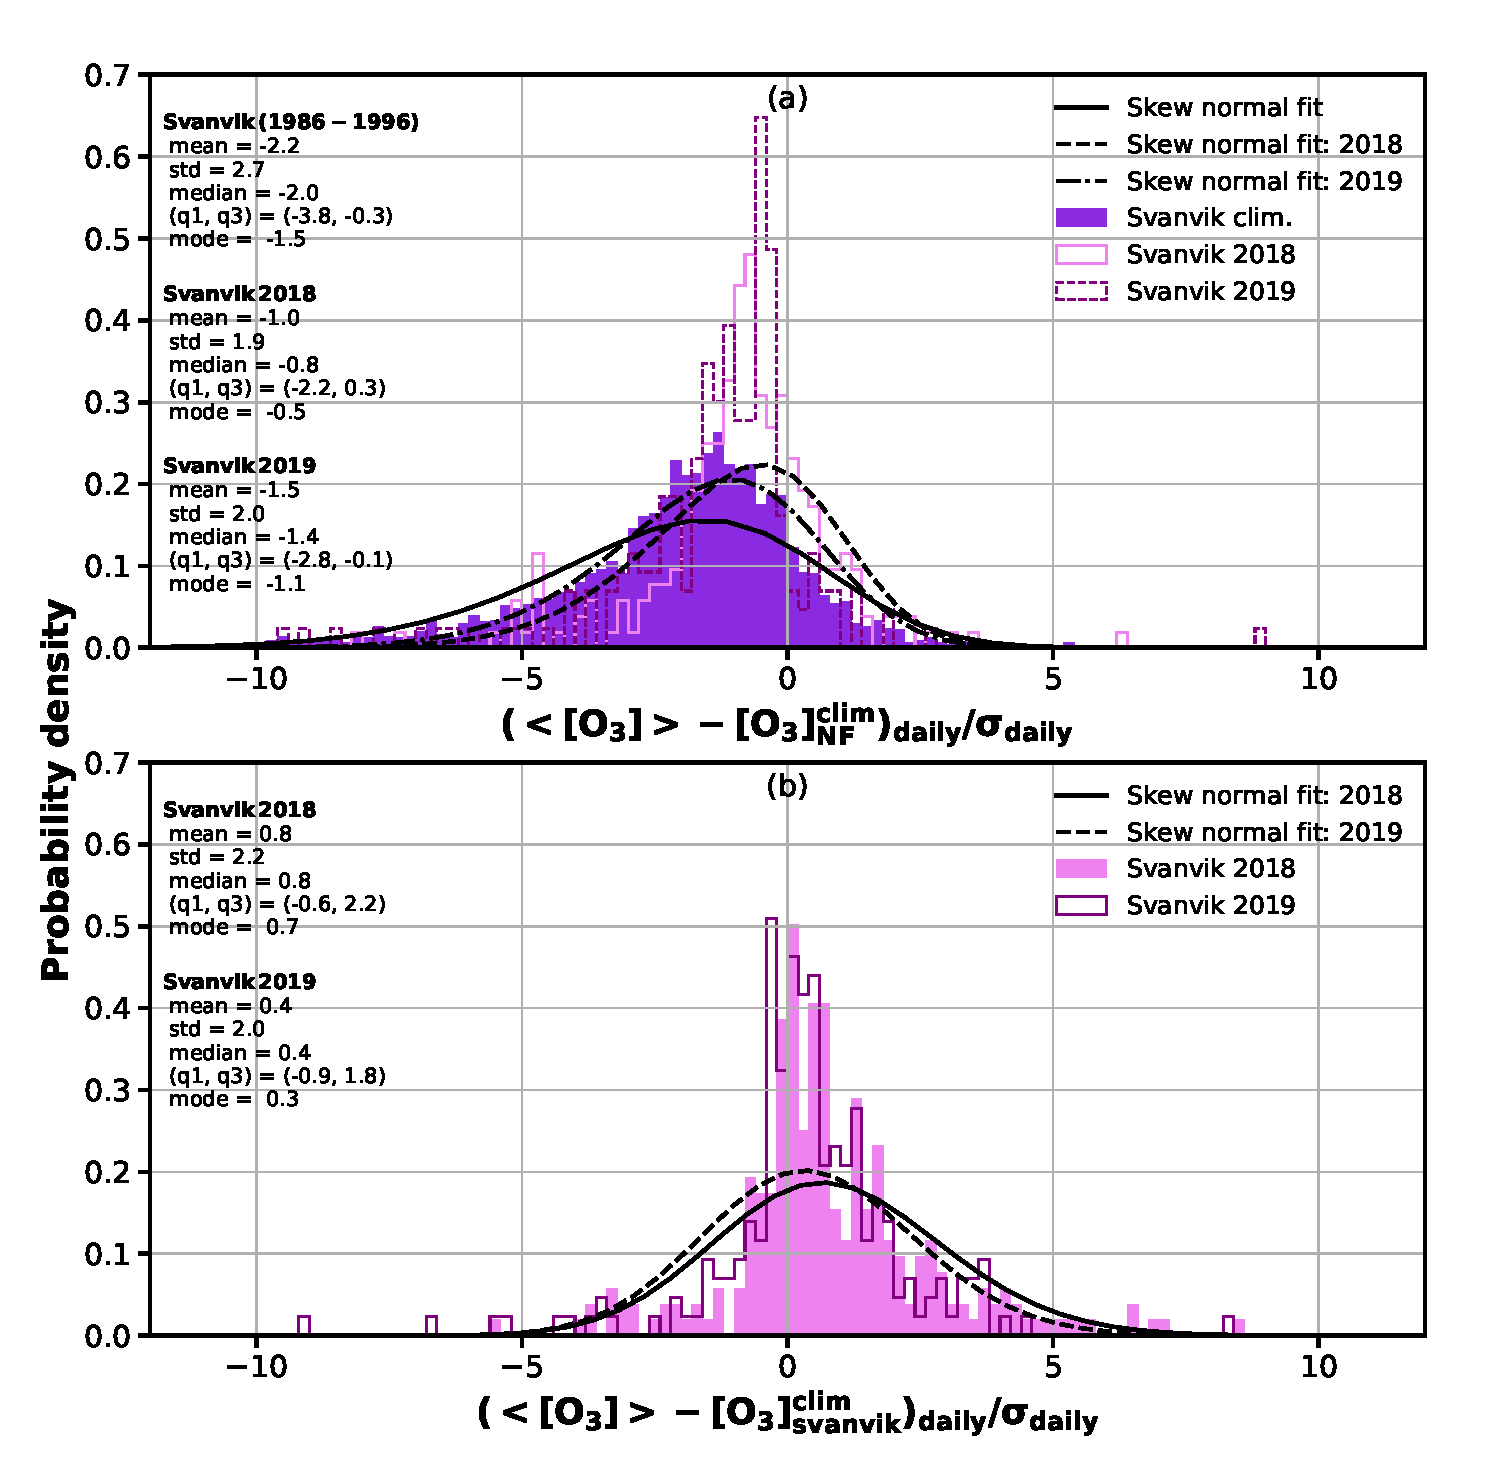
\includegraphics[width=12cm]{ozone_climatology_fenoscandic_obs_test-Svanvik}
  \caption{Student's t-test assuming same sample uncertainty in both, climatology and 2018/19 observations at Svanhovd with respect to derived climatologies for (a) Northern Fennoscandia; (b) Svanvik. \chem{\Delta[O_3]} in Fig.~\ref{fig:ozone_climatology_fenoscandic_obs_residuals}a) are significantly different from zero-hypothesis on the $2\,\sigma$,  $1\,\sigma$ level, respectively. \chem{\Delta[O_3]} in Fig.~\ref{fig:ozone_climatology_fenoscandic_obs_residuals}b) are not significantly different from zero-hypothesis.}
  \label{fig:ozone_climatology_fenoscandic_obs_test-Svanvik}
\end{figure*}

\begin{figure*}[th]
  \centering
  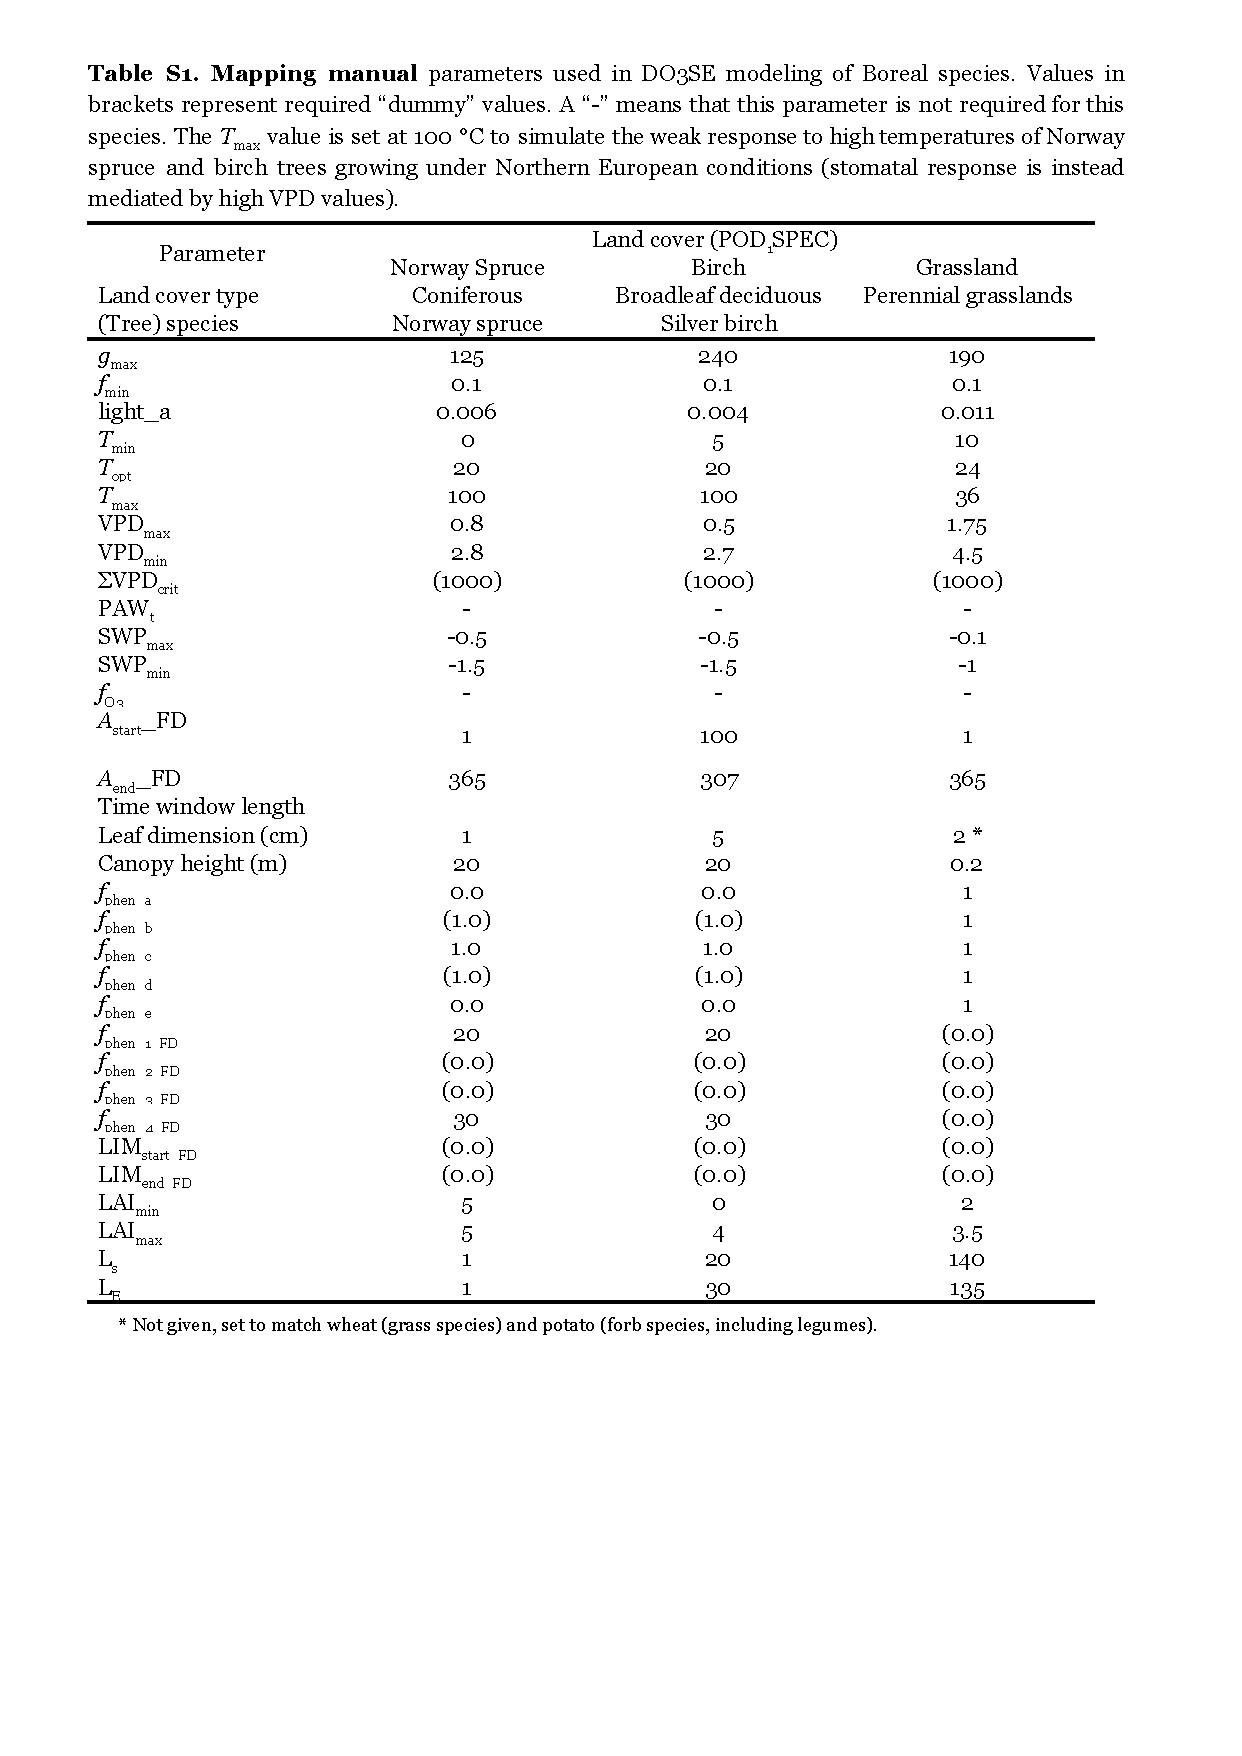
\includegraphics[width=1\textwidth]{supplements/supplement_do3se-parameterization_v2}
\label{tab:do3se_mm_param}
\end{figure*}

\begin{figure*}[t]
  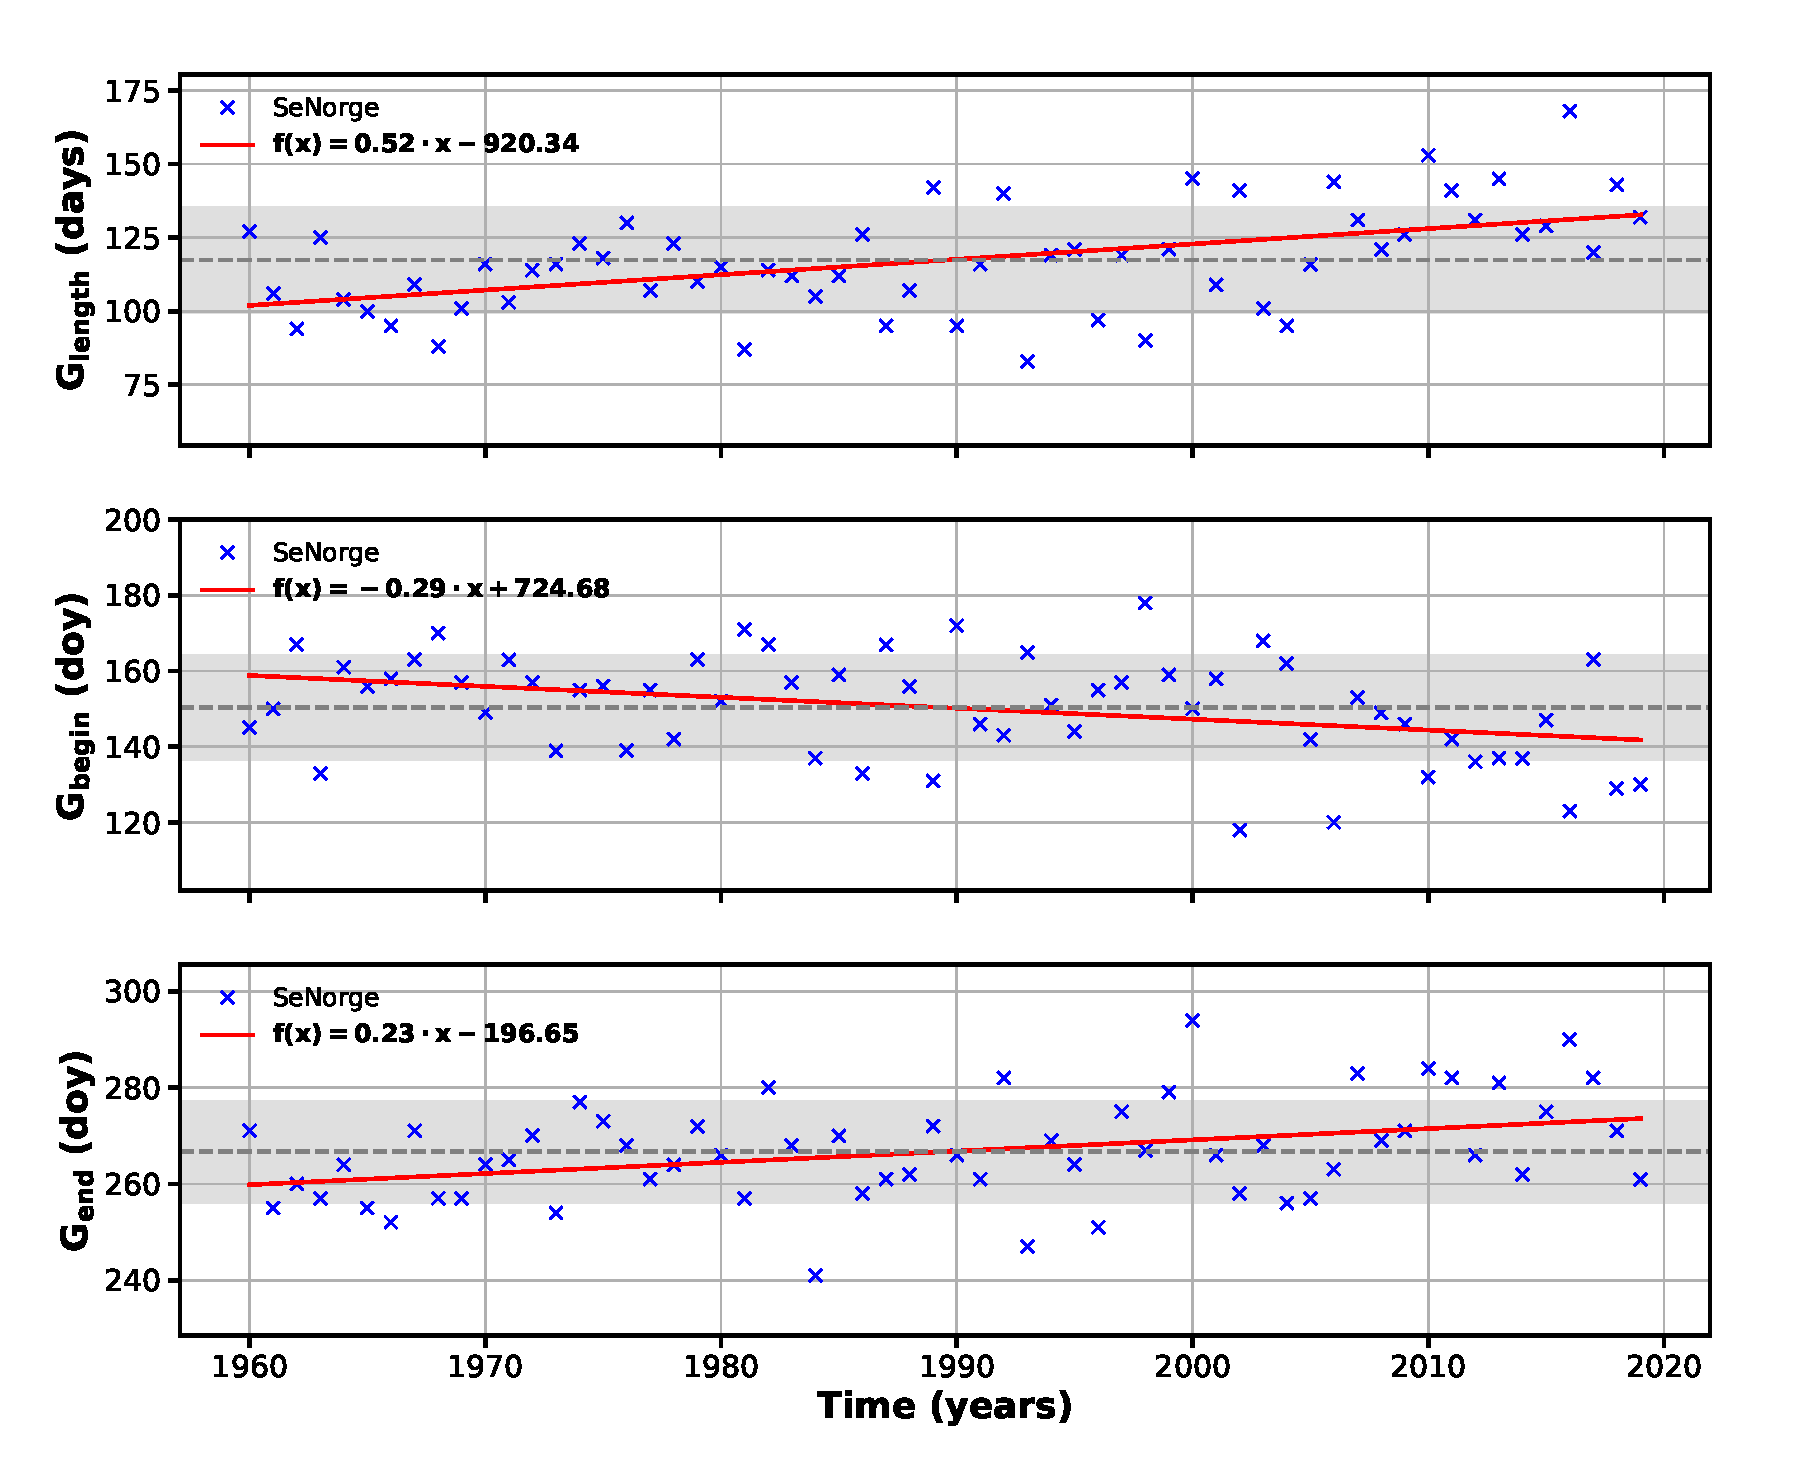
\includegraphics[width=12cm]{greening_season_change_Svanvik}
  \caption{Estimated shift and prolongation of growing season at Svanhovd over the past 6 decades based on data from \citet{SeNorge}.}
  \label{fig:greening_season_change_Svanvik}
\end{figure*}


%\begin{figure*}[t]
%  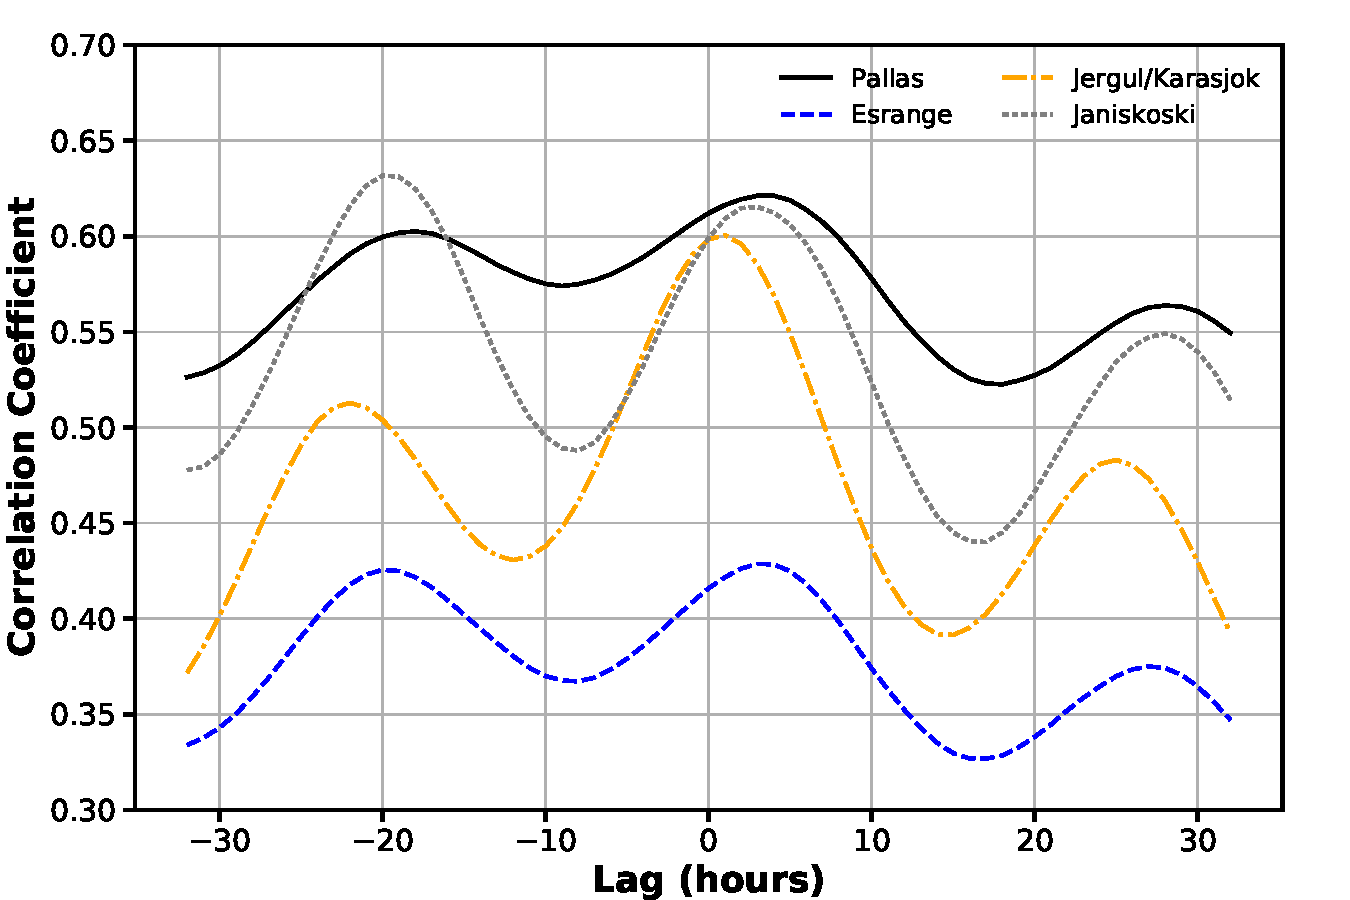
\includegraphics[width=12cm]{ozone_observation_timelag_svanvik}
%  \caption{Temporal correlation of \chem{[O_3]} data at Svanvik with other ozone monitoring stations in northern Fennoscandia. A negative lag means that Svanvik lags behind, while a positive lag mean the other station lags behind. The highest correlation with Pallas/Esrange is found at a time lag of $3\,\unit{h}$, for Jergul/Karasjok at $1\,\unit{h}$, and for Janiskoski at $-20\,\unit{h}$.}
%  \label{fig:time_lag_correlation}
%\end{figure*}

%\begin{figure*}[t]
%  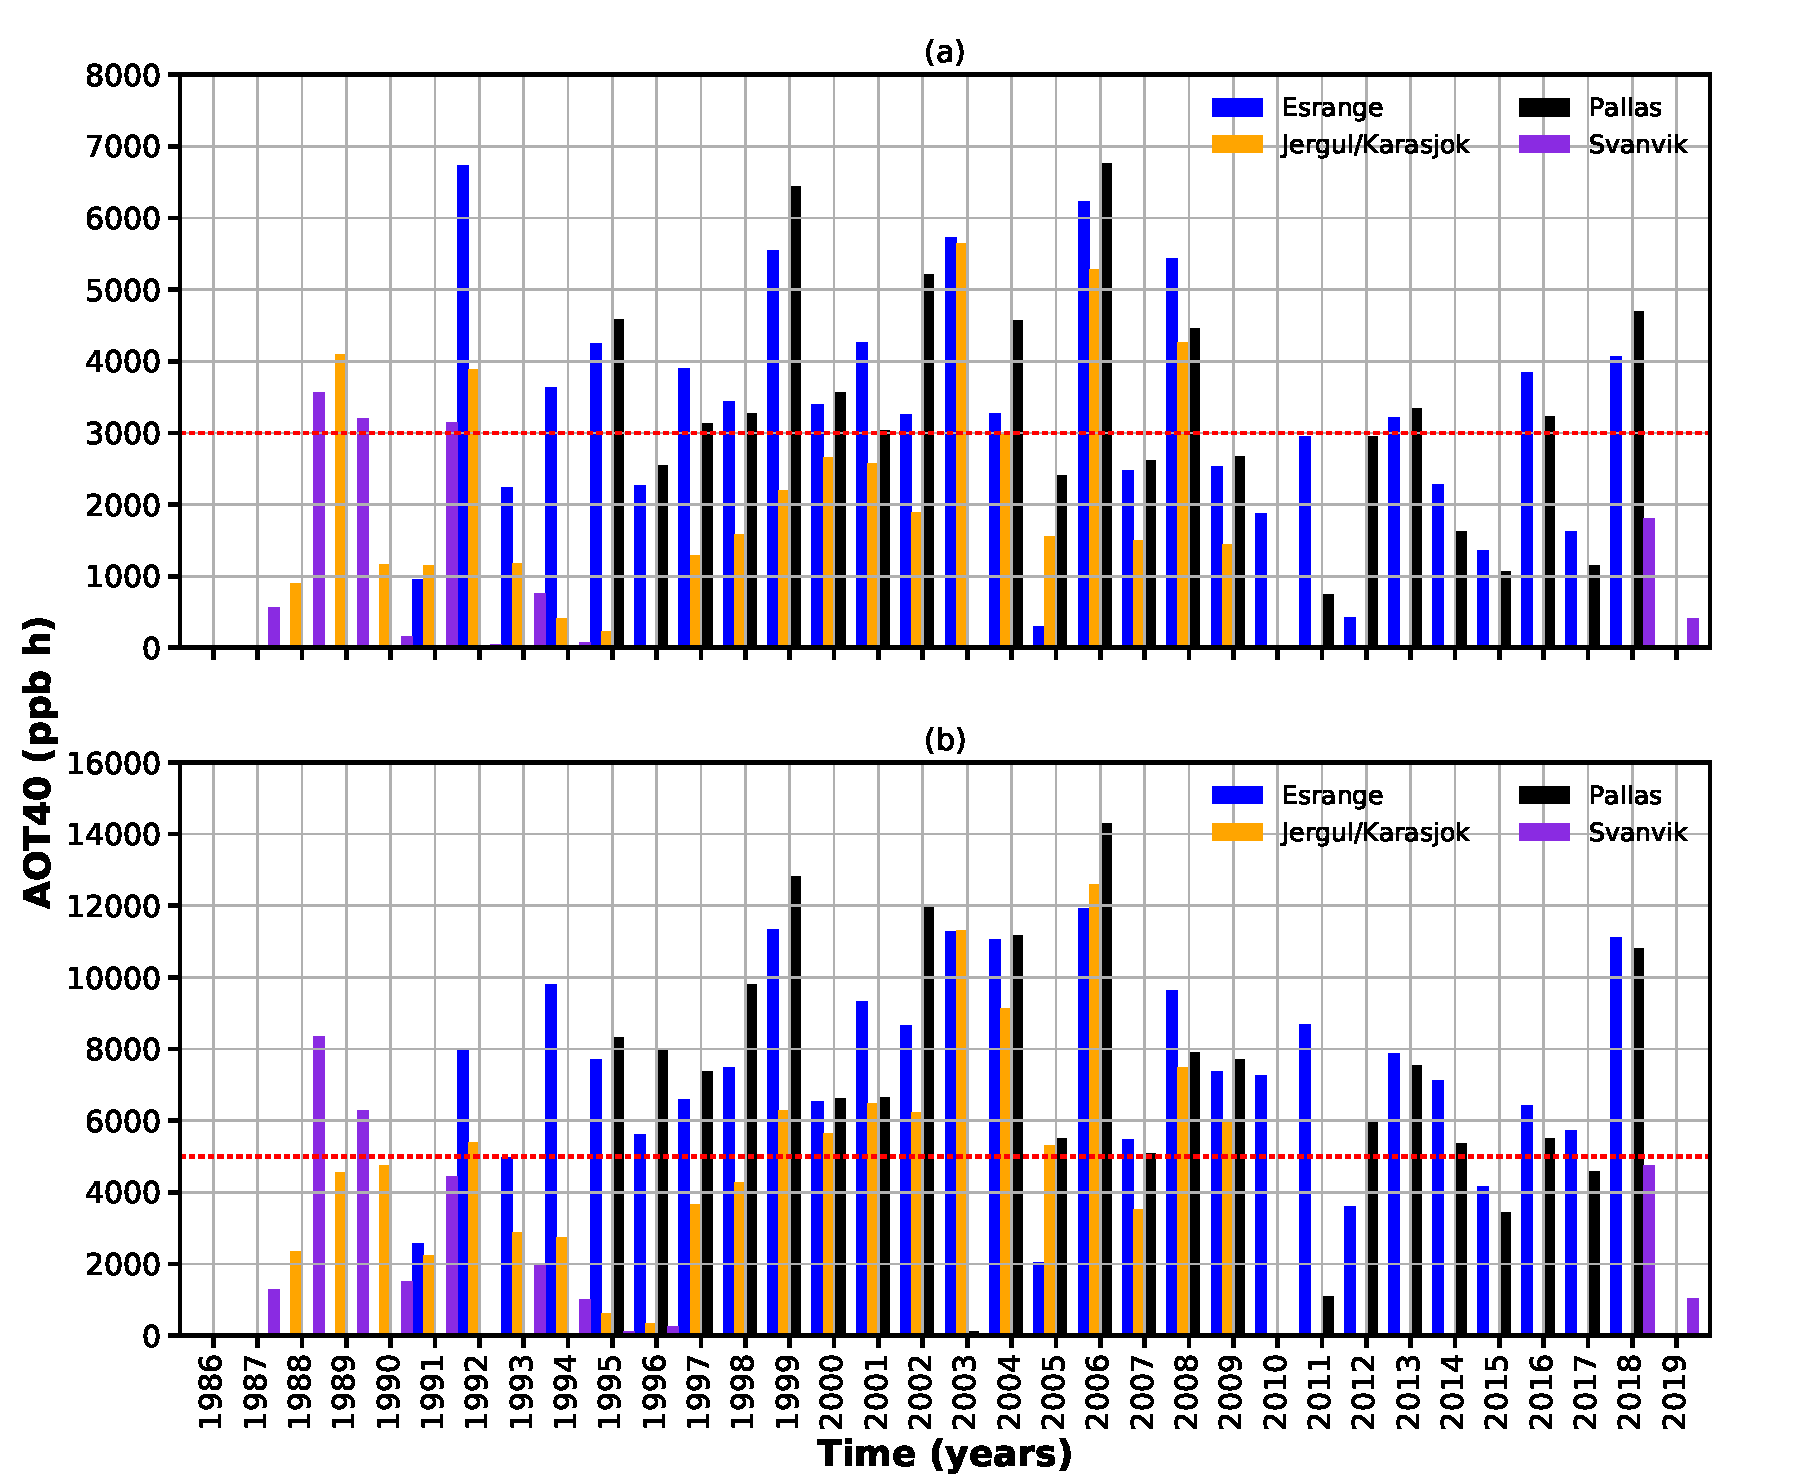
\includegraphics[width=12cm]{ozone_fennoscandic_obs_aot40}
%  \caption{Integrated AOT40 for various sites in northern Fennoscandia over the course of 33 years. For simplicity, we integrated hourly ozone between $1\,\unit{am}-11\,\unit{pm}$ in any case, although a night time light intensity $> 50\,\unit{W\,m^{-2}}$ is only measured during midnight sun conditions. Since night time \chem{[O_3]} is mostly below $40\,\unit{ppb}$, the such induced high bias in spring should be tolerable. The dashed red lines indicate the respective threshold given by the EU directive. (a) May 1 -- July 31 (b) April 1 -- September 30.}
%  \label{fig:fennoscandic_aot40}
%\end{figure*}



\end{document}
